\documentclass[a4paper,12pt]{scrreprt}
    %% Used for changing geometry of the page
    %% Cover page text cannot overlay cover sketching/style 
    %% https://ctan.org/pkg/geometry?lang=en
\usepackage{geometry}
    %% Changes language of some packages protocols
    %% e.g., when captioning images: Figure 1. -> Figura 1.
    %% https://ctan.org/pkg/babel?lang=en
\usepackage[portuguese]{babel}
    %% Used for special fonts
    %% Cannot be compiled with pdflatex
    %% https://ctan.org/pkg/fontspec?lang=en
\usepackage{fontspec}
    %% Arial FONT
    \setmainfont{Arial}

\usepackage{comment}
\usepackage{pgffor} % for the \foreach loop

\usepackage{datetime}

\usepackage{advdate}

    %% More colors and color options
    %% https://ctan.org/pkg/xcolor?lang=en
    %% https://ctan.org/pkg/colortbl?lang=en
\usepackage{xcolor,colortbl}
    %% More tabular options, like dashed/dotted lines
    %% https://ctan.org/pkg/arydshln?lang=en
\usepackage{arydshln}
    %% List of acronyms
    %% https://ctan.org/pkg/nomencl?lang=en
\usepackage[intoc]{nomencl}
    %% Must be called to init nomencl environment  
    \makenomenclature
    %% More images options/settings
    %% https://ctan.org/pkg/graphicx?lang=en
\usepackage{graphicx}
    %% Defining subdirectories to image path enviornment
    %% \graphicspath{{sub1}{sub2}...{subN}}
    \graphicspath{{images}}
    
    %% used to handle cross-referencing commands in LaTeX to produce hypertext links in the document
    %% https://ctan.org/pkg/hyperref?lang=en
\usepackage{hyperref}
    %% math environments
    %% https://ctan.org/pkg/amsmath?lang=en

    %% settings
    \hypersetup{
        colorlinks,
        citecolor=black,
        filecolor=black,
        linkcolor=black,
        urlcolor=black
    }

\usepackage{amsmath}
    %% Defining backgrouns, used to make the cover
    %% https://ctan.org/pkg/background?lang=en
\usepackage[some]{background}
    %% Used to make drawings or complex graphics
    %% http://pgf.sourceforge.net/pgf_CVS.pdf
\usepackage{tikz}
    %% Tikz library to point operations ((x1,y1) + (x2,y2))
    \usetikzlibrary{calc}
\usepackage{enumitem}

\usepackage{graphicx}

\usepackage[export]{adjustbox}

\usepackage{comment}

\usepackage{listings}
\usepackage{xcolor}

\lstdefinestyle{sharpc}{language=[Sharp]C, frame=lr, rulecolor=\color{blue!80!black}}


%% Defining sfdefault font and default font for document
\renewcommand{\familydefault}{\sfdefault}

\setcounter{secnumdepth}{3}

%% Costume made cover 
%% From there you can use \makecover command to build the cover

%==========================================================================
% DOCUMENT
%==========================================================================

\begin{document}
%% Blue cover color
\definecolor{titlepagecolor}{RGB}{54,95,145}

%==========================================================================
% COLORED BAR ON THE LEFT SIDE
%==========================================================================

\backgroundsetup{
    scale=1, 
    angle=0, 
    opacity=1,
    contents={
        \begin{tikzpicture}[remember picture,overlay]
            \path [fill=titlepagecolor] 
                (current page.north west) -- ($(current page.north west) + (5,0)$)
                -- ($(current page.south west) + (5,0)$)-- (current page.south west); 
            \node[color=white] at ($(current page.south west) + (3,4)$) {\bfseries {\fontsize{120}{60} \textsf{LI}}};
            \node[color=titlepagecolor] at ($(current page.south west) + (5.8,4)$) {\bfseries {\fontsize{120}{60} \textsf{4}}};
        \end{tikzpicture}
    }
}

%==========================================================================
% TITLE PAGE INFO
%==========================================================================

%% Changes values in this field to show information in the cover and back cover about your team/project


%% TITLE
\title{Gestor de Montagem LEGO}

%% AUTHORS
\author{
    André Carvalho$($a100818$)$
  \quad
    Gonçalo Gonçalves$($a100833$)$
  \quad
    Gustavo Barros$($a100656$)$
  \quad
    Nuno Peixoto$($a93244$)$
  \quad
    Pedro Ferreira$($a97646$)$
}

%% Date

\date{\today}

%% Course
\newcommand{\Course}{Licenciatura em Engenharia Informática}

%% Department
\newcommand{\Department}{Escola de Engenharia}

%% UniName
\newcommand{\UniName}{Universidade do Minho}

%% UniPic
\newcommand{\UniPic}{
\includegraphics[scale=0.09]{images/uminho.png}}

%% University 
\newcommand{\University}{
    \begin{flushleft}
        \UniPic
    \end{flushleft}
    \textcolor{gray}{\small\textbf{\textsf{\UniName}}}\par
    \textcolor{gray!80!white}{\small{\textsf{\Department}}}\par
    \textcolor{gray!70!white}{\small{\textsf{\Course}}}
}

%% UC
\newcommand{\UC}{
    \begin{flushleft}
        \par\textcolor{titlepagecolor}{  \LARGE\textbf{\textsf{Unidade Curricular de \\ Laboratórios de Informática IV}}}
    \end{flushleft}
}

%% School Year
\newcommand{\SchoolYear}{
    \small{\textsf{Ano Letivo de 2024/2025}}}


%% Define new command to show title, author and date
\makeatletter
\let\Title\@title
\let\Author\@author
\let\Date\@date
\makeatother

%==========================================================================
% CLASSIFICATION SECTION 
%==========================================================================

%% School Year
\newcommand{\ReceptionDate}{}
%% Responsible
\newcommand{\Responsible}{}
%% Evaluation
\newcommand{\Evaluation}{}
%% Observations
\newcommand{\Observations}{}





%% MAKETEMPLATE
\newcommand{\makecover}{

%==========================================================================
% BEGIN COVER PAGE 
%==========================================================================

%% Removes page number on footer
\thispagestyle{empty}

%% No indentation 
\setlength{\parindent}{0em}

%% Put Background defined on \backgroundsetup, in this page
\BgThispage

%% Changing geometry to prevent overlay with text
%% At the end of back cover, geometry is default with \restoregeometry
\newgeometry{top=5cm,left=6cm,right=3cm,bottom=2cm}

%% builds university info defined previously
\University
\vspace{1cm}
%% builds curricular unity info defined previously
\UC
%% builds school year info defined previously
\SchoolYear

\vspace*{5cm}
%% bigger space (i think its the default one) between paragraphs 
\setlength{\parskip}{1em}

%% builds title info defined previously
\par\textbf{\textsf{\huge\Title}}
\vspace{1cm}
%% builds author(s) info defined previously
\par\Author

\vspace{0.5cm}

%% builds date info defined previously
\par\Date
\restoregeometry
\pagebreak

%==========================================================================
% END COVER PAGE 
%==========================================================================

%==========================================================================
% BEGIN BACK COVER PAGE 
%==========================================================================

%% Removes page number on footer
\thispagestyle{empty}

% Changing look of lines in tabular environment 
% Dashed -> dotted 
%% length of dashes
\setlength\dashlinedash{0.3pt}
%% space between dashes
\setlength\dashlinegap{1.5pt}
%% width of dashes
\setlength\arrayrulewidth{1.1pt}


%% This values can be changed in the preamble
\begin{flushright}
\begin{tabular}{ :p{4cm}:p{4cm}: } 
\hdashline
Data de Receção & \ReceptionDate \\ [2ex]
\hdashline
Responsável & \Responsible \\ [2ex]
\hdashline
Avalição & \Evaluation \\ [2ex]
\hdashline
Observações & \Observations \\ [7ex]
\hdashline
\end{tabular}
\end{flushright}


\vspace{10cm}
\begin{flushleft}

%% builds title info defined previously
\par\textbf{\textsf{\huge\Title}}
\vspace{1cm}
%% builds author info defined previously
\par\Author

\vspace{0.5cm}

%% builds date info defined previously
\par\yesterday
\end{flushleft}

\pagebreak
%==========================================================================
% END BACK COVER PAGE 
%==========================================================================
}


\pagenumbering{gobble}

% builds the cover
\makecover

%% smaller footer and header size
\newgeometry{top=3cm,left=3cm,right=3cm,bottom=4cm}

%==========================================================================
% BEGIN OPCIONAL DEDICATÓRIA
%==========================================================================

%==========================================================================
% END OPCIONAL DEDICATÓRIA
%==========================================================================


%==========================================================================
% BEGIN ABSTRACT PAGE
%==========================================================================



%% Abstract name: \Large font size, flushed left and paragraph skip before abstract content
\renewenvironment{abstract}
 {\par\noindent\textbf{\Large\abstractname}\par\bigskip}
 {}

\begin{flushleft}
\begin{abstract}
    
    Neste relatório, documenta-se a primeira metade do processo de desenvolvimento coletivo duma plataforma de \textit{software} no âmbito da unidade curricular Laboratórios de Informática IV. Nesta foi proposto um programa que providenciasse uma forma de visualizar sequencialmente uma linha de produção em andamento, passo a passo.

    Assim apresenta-se o \textit{Autobrick}, um sistema que seria assentado no departamento de montagem/produção da hipotética empresa cliente, BlocoPronto Lda, que prepara modelos/conjuntos LEGO por encomenda. O Autobrick auferiria à chefia do departamento não só a mera visualização proposta, mas também a conveniente automatização de operações que lhe precedem, ligadas à gestão de peças no inventário e de encomendas a conceber.
    
    \par \textbf{Área de Aplicação}: Gestão, Produção, Visualização de Assemblagem Manual 
    \par \textbf{Palavras-Chave}: Bases de Dados Relacionais, SQL Server, Engenharia de Requisitos, Modelação Estrutural e Comportamental, UML, Casos de Uso, Interfaces Gráficos, .NET, C\#.
    
\end{abstract}
\end{flushleft}


\pagebreak

%==========================================================================
% END ABSTRACT PAGE 
%==========================================================================

%==========================================================================
% BEGIN INDEXES PAGES
%==========================================================================

%% Changes table of content name
%% Portuguese babel default : "Conteúdo"
%% Personally I prefer "índice"
\renewcommand{\contentsname}{Índice}

\tableofcontents

\pagebreak

\listoffigures

\pagebreak

\listoftables

\pagebreak

%==========================================================================
% END INDEXES PAGES 
%==========================================================================


%% Starting page numbering here
\pagenumbering{arabic}
%==========================================================================
% BEGIN #1 - INTRO
% Apresentação geral do trabalho que se pretende realizar, bem como revelar a forma como ele se irá desenvolver (ou desenvolveu) ao longo do tempo que têm para o fazer.
%==========================================================================


\chapter{Introdução}
    
    \section{Contextualização}
        
        O empresário António Silva Faria, sendo um entusiasta, colecionador e artista LEGO de longa data, considerou oportuno abrir um negócio de montagem de modelos, com maior ênfase nos modelos expositivos. 
        
        Assim, fundou-se a BlocoPronto Lda, operando segundo mail-order centralizada.
        
        A empresa foi bem-vinda na comunidade, de tal modo que a afluência de pedidos levou ao desenvolvimento do, inicialmente, pequeno negócio para grande escala.

    \section{Apresentação do Caso de Estudo}
        
        De modo ineficaz, a comunicação na empresa era totalmente feita por correio eletrónico, quer entre o cliente e a empresa (encomenda; aceitação/rejeição; faturação; apoio e esclarecimento), quer entre a empresa e o fornecedor (reposições de inventário).


        O representante pela comunicação recebe uma encomenda, que teria de encaminhar para o coordenador da linha de montagem, este teria que verificaria o stock e a viabilidade da conceção da encomenda, após isto iria reponder ao representante se seria possível concretizar a encomenda. Só após este processo, totalmente à mercê da habilidade logística de dois encarregados de áreas distintas, é que o cliente saberia se a encomenda seria realizada ou não. Para um coordenador da linha de montagem verificar esta viabilidade, seria necessária uma consulta da lista de peças necessárias, obtida no \textit{website} oficial LEGO, e confrontá-la com o inventário disponível.
        
    \newpage
    \section{Motivação e Objectivos}
        
        Com o passar do tempo, a procura pela empresa cresceu consideravelmente. Com este crescimento tornou-se evidente que a logística da empresa não era eficaz: havia um volume absurdo de emails e frequência das consultas comparativamente à quantidade de encomendas efetivamente concebidas - um calcanhar de Aquiles na escalabilidade e no \textit{throughput} das linhas de montagem. Claro se torna que isto se deve ao facto de a empresa depender de plataformas que não foram desenvolvidas para o uso que estão a ter. Problema que a administração quer resolver.


        Em média, funcionários das empresas com cargo interativo ocupam cerca de 28\% e 20\% do seu tempo laboral na gestão de emails e na busca por informação interna, respetivamente\cite{Chui2012}. No caso da BlocoPronto, segundo análises internas do ano anterior, estes valores são 39\% e 26\%, respetivamente, o que fez suscitar a vontade de criar uma plataforma adaptada às necessidades logísticas da empresa, que permitisse alocar mais tempo para a montagem. Com isto em mente, a nova plataforma disponibilizaria, de forma unificada:

        \begin{enumerate}
            \item Consulta a Referências dos Modelos LEGO
            \begin{itemize}
                \item Armazenamento interno dos manuais instrucionais;
                \item Visualização passo-a-passo das etapas de montagem na linha.
            \end{itemize}

            \item Gestão sobre Encomendas de Montagem
            \begin{itemize}
                \item Listagem de encomendas pendentes à medida que chegam;
                \item Teste automático da viabilidade de conceção da encomenda segundo o inventário;
                \item Processamento (aceitação/rejeição) da encomenda segundo a viabilidade;
                \item Ordenação em fila das encomendas a conceber.
            \end{itemize}
        
            \item Manutenção de Inventário
            \begin{itemize}
                \item Listagem das peças atualmente disponíveis e em que respetivas quantidades;
                \item Criação de pedidos para reposição de inventário.
            \end{itemize}
        \end{enumerate}

    \newpage
    \section{Estrutura do Relatório}
    
        O desenvolvimento do sistema conta com - até ao momento de publicação - cinco fases, cada qual correspondente a um capítulo no índice. Eis uma curta descrição do que cada uma aborda:
    
        \begin{enumerate}
            \item Reflete sobre o contexto fundamental (a razão de ser) do sistema, o que colmataria (e como, de grosso modo) e o que implicaria em recursos e logística.
            \item Revela a estipulação final dos requisitos do sistema e, adicionalmente, relata-se a estratégia que a equipa encarregada usou, dentro do contexto da hipotética empresa, para os obter.
            \item Com base nos requisitos, apresentam-se os modelos e especificações geradas, em registo conceptual e corrente, para ajudar à definição da arquitetura e do comportamento sob utilização.
            \item É definida e explicada uma estrutura concreta para a camada de dados.
            \item Expõem-se esboços da interface gráfica, tais estes que também serviriam de material a expôr ao cliente hipotético.
        \end{enumerate}

    O capítulo 6 dá como concluída esta primeira metade do desenvolvimento com uma crítica retrospetiva das suas fases e um comentário sobre a metade seguinte.   

    \newpage
    \section{Justificação e Utilidade do Sistema}
        O sistema vem colmatar as barreiras impostas às montagens e o atraso na sua iniciação causados pela necessidade de confirmação humana para responder a encomendas e pelo uso de plataformas disjuntas e inadaptadas. Este vem também permitir um aumento da frequência e velocidade de resposta a pedidos de montagem e, consequentemente, de modelos montados e eficiência laboral.

        
        Dum modo sucinto, sentir-se-ão os seguintes efeitos na empresa:
        \begin{itemize}
            \item Aumento da parcela temporal que os montadores usam para efetivamente montar durante o horário de trabalho, dado o fluxo mais conveniente e automatizado que se introduz;
            
            \item Redução da dependência inter-departamento de cariz substituível por registos elaborados por máquina;
            
            \item Melhoria da reputação com os clientes, desprendendo o representante das funções notificáveis diretamente pela produção, este torna-se mais flexível para relações públicas;
            
            \item Aumento da quantidade de modelos montados por dia;
            
            \item Aceleração do processo de integração de novos montadores, vista a simplificação do fluxo das diferentes tarefas inerentes ao cargo.
        \end{itemize}
        
        Tendo em consideração a séria possibilidade de crescimento da empresa e aumento de receita com esta otimização logística, os custos de desenvolvimento e manutenção do software (que não aumentam com a quantidade de modelos disponíveis e/ou encomendas recebidas) consideram-se, facilmente, justificáveis.
        
        Assim, o investimento vê-se viável e bastante adequado para o futuro da empresa.

    \newpage       
    \section{Identidade do Projeto}
        
        \textbf{Designação do Projeto:}
        \begin{itemize}
            \item[] Autobrick - Serial LEGO Building Manager 
        \end{itemize}
         
        \textbf{Equipa de Trabalho e Desenvolvedores:}
        \begin{itemize}
            \item[] André Carvalho, Gonçalo Gonçalves, Gustavo Barros, Nuno Peixoto, Pedro Ferreira
        \end{itemize}
    
        \textbf{Tempo de Desenvolvimento:}
        \begin{itemize}
            \item[] 16 Setembro 2024 a 20 Janeiro 2025
        \end{itemize}

        \textbf{Síntese:}
        \begin{itemize}
            \item [] Plataforma auxiliar duma linha de montagem de modelos LEGO com base em encomendas recebidas. Inclui:
            \begin{itemize}
                \item \textit{Rastreio de inventário.}
                    Mantém um registo do inventário atual e permite criar pedidos de reposição de peças.
                \item \textit{Processamento de encomendas.}
                    Permite consulta dos modelos requisitados numa encomenda recebida e informa se é viável consoante o inventário, agilizando a decisão quanto à conceção dela.
                \item \textit{Visualização de montagem.}
                    Providencia consulta da sequência de montagem de cada modelo.
            \end{itemize}
        \end{itemize}
        \textbf{Público-Alvo, Área de Atuação:}
        \begin{itemize}
            \item[] Coordenador de Linha de Montagem na empresa BlocoPronto
        \end{itemize}

    \newpage
    \section{Identificação dos Recursos Necessários}
    
    Os recursos necessários para o desenvolvimento do sistema são divididos em duas partes: o software e o hardware. O primeiro diz respeito a todo o tipo de programas desenvolvidos ao longo do projeto, desde a sua criação à sua implementação. Já o segundo refere-se a todo o equipamento e ferramentas necessários de modo a conseguir desenvolver e implementar o sistema.

        \textbf{Software:}
        \begin{itemize}
            \item Figma, Visual Paradigm (para modelação e maquete)
            \item Microsoft Visual Studio, VSCode, \textit{framework} .NET (para codificação)
            \item Microsoft SQL Server (para sistema de dados)
            \item Overleaf, Google Docs (para relatório)
            \item Microsoft Excel (para planeamento)
        \end{itemize}

        \textbf{Hardware:}
        \begin{itemize}
            \item Computadores para codificação do sistema;
            \item Dispositivos para armazenamento de dados;
            \item Servidor para hospedagem da base dados.
        \end{itemize}
    
    \newpage            
    \section{Maquete do Sistema}

        Foi esboçada uma maquete do sistema (Figura 1.1) com o intuito de conseguir demonstrar, duma forma primitiva, um pouco de todas as camadas envolventes (dados, lógica e interface) e como se interligariam.
        
        Cada dos cartões laranja é intitulado no canto superior esquerdo e, salvo ser de intenção meramente interfacial, associado a um marcador colorido que indica a que componente abstrata do sistema corresponde.

        \textbf{Gestão de Utilizadores} alberga a \textit{Autenticação} pois seria por este componente que se registariam as credenciais de acesso, contra quais se confrontaria à validade duma tentativa de entrada em conta.

        \textbf{Gestão de Encomendas} engloba \textit{Encomendas Pendentes} e \textit{Fila de Montagem} pois ambos os cartões se dedicam a operações ou visualizações baseadas nos dados sobre as encomendas.

        \textbf{Gestão de Inventário} segue o mesmo princípio para \textit{Inventário de Peças} e \textit{Pedidos de Reposição} mas baseado nos registos de peças ou disponíveis ou em pedido.

        \textbf{Gestão de Modelos} idem para \textit{Catálogo de Modelos}; adicionalmente, como a sequência de montagem dum modelo é uma característica única a este, \textit{Visualização de Montagem} foi colocada sob este componente.

        As setas servirão para indicar o fluxo de navegação pelo sistema, enquanto que as descrições em janela azul indicarão as formas com que os dados podem ser modificados consoante o cartão em questão.
        
        \begin{figure}
            \centering
            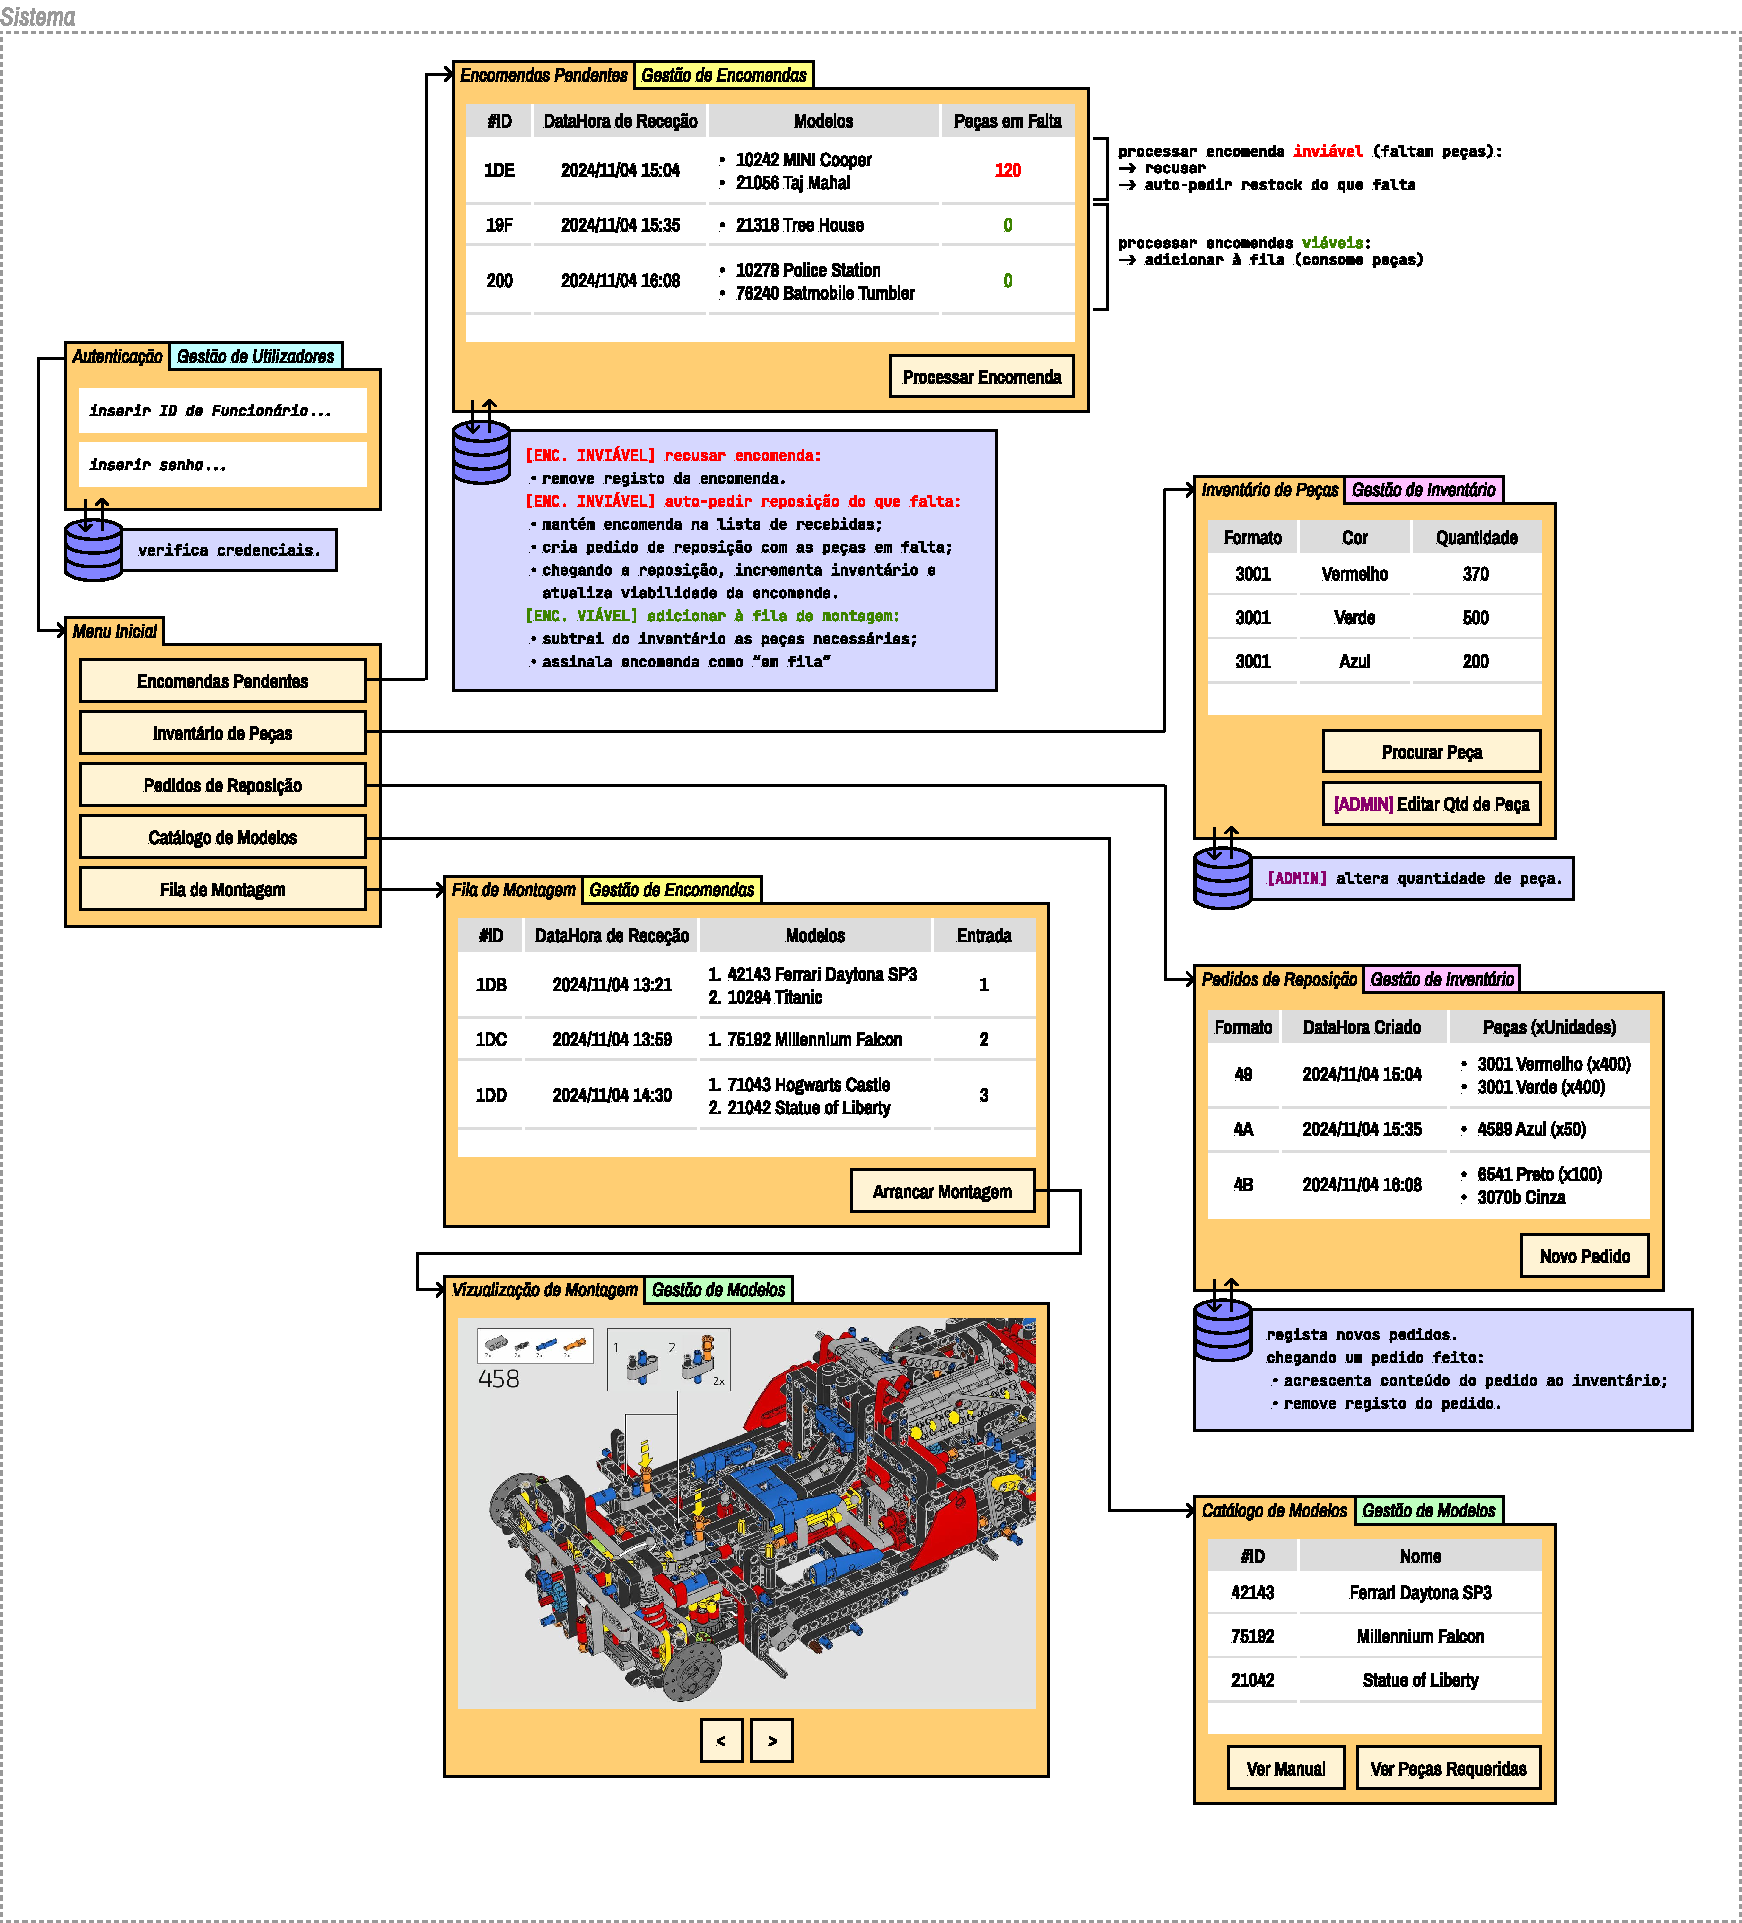
\includegraphics[width=\textwidth]{images/cap1_maquete.pdf}
            \caption{Maquete do sistema.}
            \label{fig:maquete}
        \end{figure}

        
    \newpage
    \section{Métricas de Sucesso}

    O sucesso do sistema pode ser avaliado recorrendo a uma sondagem, posterior à introdução do programa na empresa, segundo os seguintes critérios:
    \begin{enumerate}
        \item Medidas Industriais
            \begin{itemize}
                \item A implementação do sistema contribuiu para aumentar a eficiência da linha de montagem?
                \item Houve um aumento na média de encomendas processadas por dia?
            \end{itemize}
        \item Medidas de Utilização 
            \begin{itemize}
                \item Qual a média de aprovação dos funcionários em relação à adoção do novo sistema?
                \item Quanto tempo foi necessário para os funcionários se habituarem à nova interface?
            \end{itemize}
        \item Medidas Financeiras  
            \begin{itemize}
                \item O sistema causou crescimento significante nos lucros?
                \item Em quanto tempo o sistema conseguiu cobrir o custo inicial de investimento?
                \item Os custos recorrentes de manutenção justificam-se perante os resultados obtidos?
            \end{itemize}
    
    
    \end{enumerate}
     
    \newpage
    \section{Plano de Desenvolvimento}
    
        Com o intuito de preparar e planear o desenvolvimento de todo o projeto, foi delineado um diagrama de Gantt, ilustrado na figura seguinte. A escolha deste tipo de diagrama, deve‐se a vários fatores, entre eles: a clara visualização cronográfica das diversas tarefas, a facilidade de alocação de recursos humanos a cada tarefa e, finalmente, a possibilidade de planeamento a longo prazo.
        
        A localização temporal das várias tarefas no desenvolvimento depende do que requeiram de base. Por exemplo, a modelação requer requisitos, logo a engenharia de requisitos precede a modelação. A modelação estrutural é a base para a definição do sistema de dados, logo esta última vem a seguir.

        Na primeira reunião de equipa, estabeleceu-se a realização de reuniões semanalmente e distribuiram-se tarefas pela primeira vez. Tal distribuição foi sendo modificada à medida que se avançava e tomava melhor ideia do tempo que necessitariam. Deste modo, o planeamento de trabalho tomou a metodologia \textit{agile} como inspiração. 
        
        \begin{figure}[h!]
            \centering
            \includegraphics[width=\textwidth]{images/gantt.png}
            \caption{Diagrama de Gantt}
            \label{Diagrama de Gantt}
        \end{figure}
    

%==========================================================================
% END #1 - INTRO
%==========================================================================
%==========================================================================
% BEGIN #2 - LEVANTAMENTO/ANALISE DOS REQUISITOS
% Levantamento e redação dos requisitos do sistema a desenvolver, identificando de forma concreta e detalhada as funcionalidades (e restrições) que o sistema deverá ter de forma a satisfazer as necessidades apresentadas pelos seus promotores (stakeholders) e utilizadores. O processo de levantamento e de análise de requisitos constitui uma das partes mais importantes (senão a mais importante) de um projeto de engenharia de software.

\newcommand{\freq}[3]{
    \parbox{\dimexpr\textwidth-2em}{
        \subsection{#1}
        \begin{itemize}[left=1em]
            \item \textbf{Definição:} #2
            \item \textbf{Especificação:} #3
        \end{itemize}
    }
}

\newcommand{\nreq}[2]{
    \parbox{\dimexpr\textwidth-2em}{
        \subsection{#1 (N/ Funcional)}
        \begin{itemize}[left=1em]
            \item \textbf{Definição:} #2
        \end{itemize}
    }
}


%==========================================================================

\chapter{Levantamento e Análise dos Requisitos}
    
    \section{Estratégia/Método de Levantamento}

    O processo de levantamento de requisitos partiu de uma reunião com o diretor executivo, o contabilista e o representante de comunicação. Aqui, foram esclarecidos os principais pontos fracos relativos a reposições de inventário e receção de encomendas.
    
    De seguida, fez-se inquéritos ao nível da linha de montagem. Foram registadas as sugestões dos coordenadores de linha, visto este cargo ser o principal utilizador do sistema.
    
    Dada como concluída a recolha de preocupações dos utilizadores e dos \textit{stakeholders}, passou-se ao estudo das plataformas de gestão de linha de produção mais populares existentes no mercado. Esta etapa serviu para identificar características e mecanismos bem sucedidos e, portanto, passíveis de serem incluídos e/ou adaptados na nova plataforma a desenvolver.

    Nas secções seguintes, dispõe-se os requisitos levantados organizados segundo os componentes abstratos traçados na maquete (figura~\ref{fig:maquete}), cujas justificações se encontrarão na descrição precedente. Os não funcionais estão devidamente sinalizados como tal.

    \newpage
    \section{Requisitos sobre Utilizadores}

        Os requisitos seguintes partem das necessidades provenientes do componente de gestão de utilizadores. Este componente abrange operações que involvam consulta e/ou teste sobre as credenciais dos utilizadores registados. Isto implica a possibilidade de \underline{início de sessão} e respetivo \underline{fecho de sessão}. Adicionalmente, a conta correspondente à sessão atual \underline{deve ser visível}.
        
        \freq{Teste de Validade da Senha de Conta}
            {O utilizador deve ser avisado se introduziu uma senha errada para o identificador de conta que especificou.}
            {O sistema deve utilizar um registo de credenciais de modo a validar as tentativas de início de sessão por parte do utilizador.}

        \freq{Autenticação / Início de Sessão na Aplicação}
            {O utilizador deverá introduzir a sua credencial de acesso e password para iniciar sessão na aplicação.}
            {O sistema deve validar a tentativa de autenticação verificando se o par credencial de acesso e password estão registados no sistema de armazenamento de dados.}
    
        \freq{Término de Sessão na Aplicação}
            {O utilizador deve ser capaz de terminar a sua sessão após se autenticar.}
            {O sistema termina a sessão do utilizador correspondente.}

        \freq{Consultar Detalhes de Conta}
            {O utilizador deve conseguir consultar o identificador da sua própria conta enquanto se encontra em sessão.}
            {O sistema deve disponibilizar uma secção onde apresenta o identificador da conta de utilizador atualmente em sessão.}


    \newpage
    \section{Requisitos sobre Encomendas}

        Uma encomenda recém chegada terá o seu estado definido como \underline{pendente} até que o utilizador a processe. Se houver luz verde na \underline{avaliação da viabilidade da encomenda} (ou seja, comparação das peças necessárias dela contra as disponíveis), o processar da encomenda corresponderá a \underline{colocá-la em fila de montagem}. No caso contrário, ela pode ser mantida como pendente até haver mais peças ou \underline{recusada}. 

        \freq{Consultar Encomendas Pendentes}
            {O utilizador deve ter um meio de consultar todas as encomendas recebidas que ainda não foram processadas.}
            {O sistema deve manter uma lista das encomendas em estado pendente e apresentá-la ao utilizador.}

        \freq{Avaliar Viabilidade de Encomenda}
            {O utilizador, deve ser capaz de ver a viabilidade duma encomenda pendente. A viabilidade dependerá da existência de peças disponíveis em inventário suficientes para a montagem de todos os modelos requisitados por ela.}
            {O sistema, dada uma encomenda pendente, deverá comparar as peças que o inventário tem contra as que ela implica por via dos modelos requisitados. Tal deve ser apresentado ao utilizador.}
        
        \freq{Recusar Encomenda Pendente}
            {No caso de faltarem peças, o utilizador deve conseguir recusar uma encomenda pendente.}
            {O sistema deve alterar o estado da encomenda para "recusada" e filtrá-la da lista de encomendas pendentes.}

        \freq{Colocar Encomenda em Fila para Montagem}
            {O utilizador deve conseguir colocar uma encomenda em fila para subsequente montagem, assumindo que ela é viável (i.e. pode ser concebida por completo com as peças disponíveis no inventário).}
            {O sistema deverá verificar a viabilidade da encomenda. Isso implica confrontar as peças requeridas por cada modelo com as quantidades das mesmas existentes no inventário. Adicionalmente, isto assume que os modelos referidos na encomenda já estejam previamente registados.}

        \freq{Consulta de Fila de Montagem}
            {O utilizador deve conseguir visualizar todas as encomendas que previamente colocou em fila de montagem, pela respetiva ordem de colocação.}
            {O sistema deve manter uma lista das encomendas em estado "em fila" e apresentá-la ao utilizador.}

        \freq{Arrancar Fila de Montagem}
            {O utilizador, dada uma fila de montagem povoada com pelo menos uma encomenda, deve poder arrancar com a montagem - i.e. ver ordenadamente, por cada encomenda na fila, as sequências de montagem correspondentes a cada modelo que ela requisita.}
            {O sistema deverá, dada a ordem das encomendas em fila, estabelecer uma ordem para montagem dos modelos requisitados em cada encomenda individual.}

        \freq{Confirmar Montagem de Modelo em Encomenda}
            {O utilizador deve ser capaz de confirmar o final de montagem dum modelo requisitado numa encomenda. Isto dar-se-á ao concluir a visualização da sequência de montagem do mesmo.}
            {Chegando ao fim da sequência de montagem, o sistema deve apresentar uma forma de sinalizar a conclusão de montagem do modelo. Isto conduzirá à apresentação do modelo seguinte ou à alteração do estado da encomenda para como "finalizada".}    

        \nreq{Registos de Encomenda Eficientes}
            {As encomendas devem estar armazenadas no sistema de tal forma que a operação sobre várias ocorra, no máximo, em tempo linear. Isto provém da garantia de escabilidade em que o desenvolvimento do sistema se baseou.}

    \newpage        
    \section{Requisitos sobre Inventário}

        A avaliação de viabilidade duma encomenda pendente requer comparação com o atual inventário de peças, pelo que este deve ser acessível ao utilizador. Para além desta consulta, é vital que se consiga criar \underline{pedidos de reposição}, sejam estes \underline{manuais} (definidos pelo utilizador) ou \underline{automáticos} (com base nas peças em falta a uma encomenda avaliada como inviável).

        \freq{Consultar Inventário}
            {O utilizador deve conseguir consultar o inventário de peças disponíveis e respectivas quantidades.}
            {O sistema deverá manter uma lista das peças e respetivas quantidades atualmente disponíveis.}

        \freq{Realizar Pedido de Reposição Manual}
            {O utilizador deve conseguir criar um pedido de reposição do inventário com peças e quantidades à sua própria escolha.}
            {O sistema deve ter forma de criar e armazenar uma instância de pedido de reposição de peças com base na inserção direta do utilizador, para posterior acréscimo ao inventário.}   
            
        \freq{Gerar Pedido de Reposição Automático}
            {O utilizador, ao processar uma encomenda inviável, deve ter a possibilidade de criar um pedido de reposição do inventário com as peças e quantidades correspondentes ao que está em falta.}
            {O sistema deve ter forma de criar e armazenar uma instância de pedido de reposição de peças com base nas peças e quantidades que faltam a uma encomenda inviável, para posterior acréscimo ao inventário.}

        \freq{(Administrativo) Editar Quantidade Disponível de Peça}
            {O utilizador, em posse duma senha administrativa, deve ser capaz de alterar diretamente a quantidade disponível duma peça no inventário, sem ter de recorrer a pedido de reposição.}
            {Dada uma senha administrativa, o sistema deverá disponibilizar a opção de alterar a quantidade disponível duma peça no inventário.}

        \nreq{Consistência entre Pedido e Reposição}
            {A cada pedido feito deve ser correspondido exatamente o número e formato de peças reposto no inventário. A única exceção parte da aplicação do requisito 2.4.4. Contudo, é de notar que este só existe para colmatar erros de fornecimento alheios ao sistema.}

    \newpage
    \section{Requisitos sobre Modelos}

    A existência duma encomenda requer que tanto o sistema como o utilizador reconheçam cada modelo que ela requisita, de modo a saberem não só as \underline{peças necessárias} mas também qual \underline{manual de instruções a visualizar} durante a montagem.

        \freq{Consultar Catálogo de Modelos}
            {O utilizador deve ser capaz de consultar o catálogo de modelos disponíveis para produção.}
            {O sistema deverá apresentar uma lista dos modelos disponíveis para produção.}

        \freq{Visualizar Montagem de Modelo}
            {O utilizador deve conseguir visualizar a sequência de montagem dum modelo, quer ordenadamente pela fila de encomendas a montar ou independentemente pelo catálogo de modelos.}
            {O sistema deve ter associado a cada modelo a sua respetiva sequência de montagem, para ser apresentada seja pelo catálogo ou devido a uma encomenda de montagem em fila que o inclua.}

        \nreq{Existência de Manual para Modelo}
            {Deve-se absolutamente garantir que um modelo terá sempre um manual de instruções respetivo, pois a visualização da sequência de montagem é dos aspetos mais importantes do sistema.}

    \newpage
    \section{Requisitos Indiferenciados}

    Especificam-se aqui requisitos não necessariamente enquadrados com nenhuma das componentes em que se subdividiu a maquete.

        \freq{Interação Gráfica Baseada em Navegador \textit{Web}}
            {O utilizador deve interagir com o sistema através duma interface gráfica desenvolvida no contexto dum navegador \textit{web}.}
            {O sistema deverá ter estabelecida uma camada que estabeleça as suas operações dadas as interações que o utilizador tem com a interface gráfica que lhe é apresentada.}

        \nreq{Compatibilidade da Interface Gráfica}
            {A interface gráfica que é apresentada ao utilizador deverá ser, dentro do possível, o mais agnóstica possível quanto ao navegador em uso.}

    \newpage
    \section{Validação dos Requisitos Estabelecidos}

    Depois de completado o processo de levantamento dos requisitos, passámos à análise dos mesmos, concluindo assim, em equipa, que se adequavam para o que era pretendido com o sistema de software a desenvolver.
    Após este acordo entre a equipa de desenvolvimento, decidimos reunir com a administração e \textit{stakeholders} da BlocoPronto para serem apresentados a especificação dos requisitos. Depois de nos ser confirmado que os requisitos correspondiam às necessidades e expectativas dos mesmos, o processo de elaboração do software pôde continuar a decorrer com normalidade.
    
    %Com o intuito de ter a certeza de que o sistema corresponde exatamente ao esperado, foram feitas várias rondas de negociação sobre a mais recente (na altura) especificação dos requisitos. Isto permitiu que se evitassem repetições de informação, expressões vagas e mecanismos fora do objetivo a cumprir.%
            
%==========================================================================
% END #2 - LEVANTAMENTO/ANALISE DOS REQUISITOS
%==========================================================================
%==========================================================================
% BEGIN #3 - ESPECIFICAÇAO/MODELAÇAO DO SOFTWARE
% Apresentação, descrição e representação dos vários elementos e serviços a serem implementados no projeto, utilizando-se, se possível, uma exposição orientada ao serviço suportada por representações UML num nível de abstração adequado.

\newcommand{\headercaso}[5]{
    \subsubsection{#1}
    \textbf{Descrição:}
    \begin{itemize}
        \item[] #2
    \end{itemize}

    \textbf{Condições:}
    \begin{itemize}
        \item[] \textbf{(Pre)} #3
        \item[] \textbf{(Pos)} #4
    \end{itemize}
}


\newcommand{\normal}[2]{
  \textbf{#1} % Title
  \begin{enumerate}[label=\arabic*.] % Numbered list
    \foreach \x in {#2} {
      \item \x % Steps, split by delimiter
    }
  \end{enumerate}
}

\newcommand{\alt}[3]{
  \textbf{#1 - no passo #2:} % Title, number, and parent step number
  \begin{enumerate}[label=\arabic*.\arabic*] % Nested numbering
    \foreach \x [count=\i] in {#3} {%
      \item[\the\numexpr#2.\i\relax.] \x % Numbering and steps
    }
  \end{enumerate}
}

%==========================================================================

\chapter{Especificação e Modelação do Software}

    \section{Apresentação Geral da Especificação}

        De modo a dar resposta aos requisitos e facilitar a discussão sobre a plataforma com \textit{stakeholders} de nível técnico variado, recorreu-se à elaboração de casos de uso (e correspondente diagrama) para modelar o seu comportamento e a um diagrama de domínio para modelar a sua estrutura.

        Continuou-se aqui a codificação por cores alusivas aos componentes abstratos estabelecidos na maquete (figura \ref{fig:maquete}): azul para utilizadores, amarelo para encomendas, verde para modelos e violeta para peças/inventário.

    \newpage
    \section{Aspetos Estruturais}

         A modelação estrutural materializa-se com um diagrama de domínio. Teve o objetivo de fomentar o debate quanto à arquitetura do sistema, em termos de componentes temáticos e entidades conceptuais, e explicar como se relacionam uns com os outros numa perspetiva estática.

        \begin{figure}[h]
            \centering
            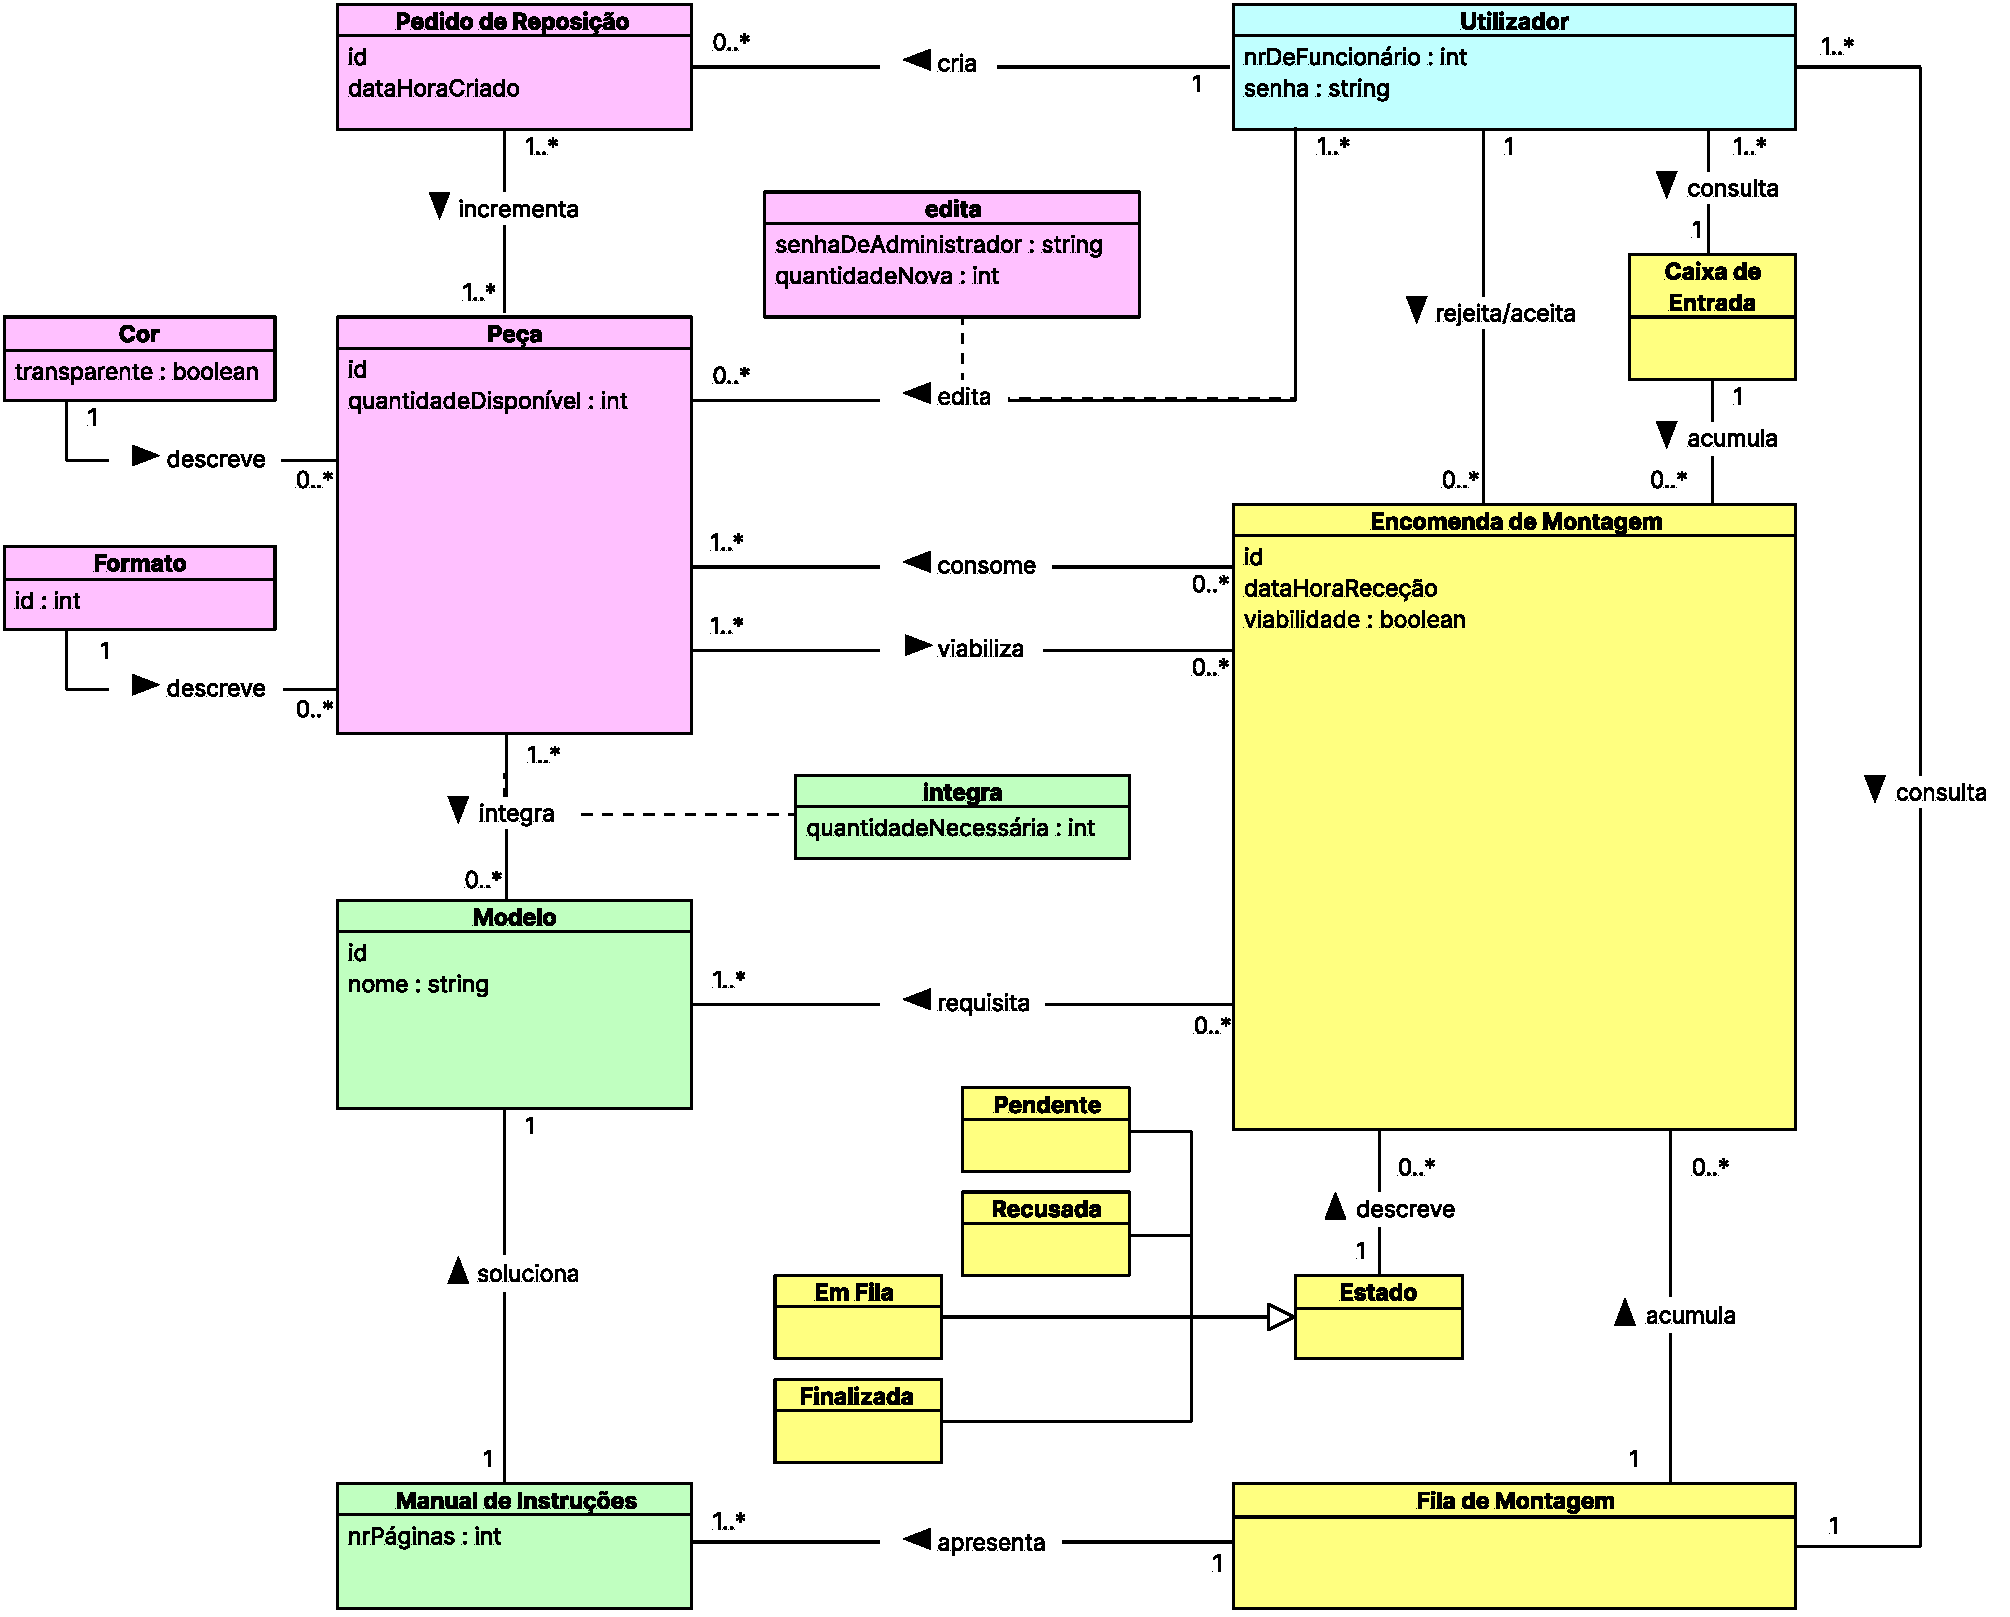
\includegraphics[width=1\textwidth]{images/cap3_diagclasses.pdf}
            \caption{Diagrama de domínio}
            \label{fig:diagclasses}
        \end{figure}

        \newpage
        \subsection{Utilizadores}

            O utilizador é caracterizado pelas suas credenciais de autenticação.

            \begin{itemize}
        
                \item \textbf{Utilizador edita Peça:} Ver requisito 2.4.4. Esta é uma operação fazível por um ou mais utilizadores. Na perspetiva oposta, a quantidade disponível de uma peça não se garante como tendo editada por qualquer utilizador.
        
                \item \textbf{Utilizador rejeita/aceita Encomenda:} Ver requisitos 2.3.3 e 2.3.4. Uma encomenda só é processada por um único utilizador. Enquanto isso, um utilizador pode processar entre nenhuma a múltiplas encomendas.
        
                \item \textbf{Utilizador consulta Caixa de Entrada:} Ver requisito 2.3.1. A consulta da caixa de entrada de encomendas só faz sentido ser realizada por um ou mais utilizadores. Tendo o propósito de colecionar as encomendas pendentes, só existe uma.
        
                \item \textbf{Utilizador consulta Fila de Montagem:} Ver requisito 2.3.5. Aplica-se o mesmo raciocínio do relacionamento anterior, mas orientado às encomendas em fila.
        
                \item \textbf{Utilizador cria Pedido de Reposição:} Ver requisitos 2.4.2 e 2.4.3. Um pedido de reposição vem a existir partido dum certo utilizador. Da perspetiva contrária, um utilizador pode criar quantos pedidos pretender, portanto, de zero a vários.

            \end{itemize}

        \newpage
        \subsection{Encomendas}

            Uma encomenda é caracterizada por um identificador, um registo temporal de receção e a sua viabilidade, esta última à mercê da presença de todas as peças necessárias. 

            \begin{itemize}
                \item \textbf{Fila de Montagem acumula Encomenda:} Ver requisito 2.3.5. A fila de montagem é uma entidade singular e universal com o propósito de colecionar encomendas, pelo que só existe uma e alberga de zero a múltiplas.
    
                \item \textbf{Estado descreve Encomenda:} O estado duma encomenda define se é apresentada no sistema (positivo caso Pendente ou Em Fila) e, se sim, se na Caixa de Entrada ou Fila de Montagem. Deste modo, cada encomenda tem obrigatoriamente um estado associado; da perspetiva oposta, um determinado estado pode estar a descrever entre zero a múltiplas encomendas em certo momento.
    
                \item \textbf{Encomenda requisita Modelo:} A empresa recebe encomendas que solicitam a montagem de um ou vários modelos. Da perspetiva oposta, um modelo específico pode ou não ser requisitado por quaisquer encomendas existentes. 
                
                \item \textbf{Encomenda consome Peça:} Como um modelo requer peças e a encomenda requisita vários modelos, o processamento duma encomenda (i.e. a colocação dela em fila) requer que sejam consumidas peças do inventário para a finalizar. Da perspetiva oposta, uma peça pode ou não ser consumida por quaisquer encomendas existentes. 
    
                \item \textbf{Fila de Montagem apresenta Manual de Instruções:} Ver requisito 2.3.6. Durante a conceção de cada modelo requisitado por uma encomenda posta em fila de montagem, é apresentado o respetivo manual de instruções. Assim, a fila de montagem é uma entidade singular que suscita a apresentação dos vários manuais.
        
            \end{itemize}

        \newpage
        \subsection{Inventário}

            Uma peça é inerentemente caracterizada por um identificador e uma quantidade disponível em inventário. Um pedido de reposição terá igualmente um identificador e também uma data/hora de criação.
        
            \begin{itemize}
                \item \textbf{Peça integra Modelo:} Um modelo LEGO é constituído por múltiplas peças, cada em quantidade necessária bem definida. 
    
                \item \textbf{Pedido de Reposição incrementa Peça:} Um pedido de reposição solicita incremento à quantidade de pelo menos uma encomenda. Na perspetiva contrária, a quantidade duma peça é incrementável por solicitação proveniente de múltiplos pedidos.
    
                \item \textbf{Cor/Formato descreve Peça:} O identificador duma peça é baseado no seu formato e cor. Assim sendo, valores específicos destas entidades podem descrever entre zero a múltiplas peças reconhecidas pelo sistema.
    
                \item \textbf{Peça viabiliza Encomenda:} Ver requisito 2.3.2. A viabilidade de conceção duma encomenda depende da existência em inventário das peças em quantidade necessária aos modelos requisitados. Assim, uma certa peça pode viabilizar de zero a múltiplas encomendas, dependendo dos modelos.
            
            \end{itemize}

        \subsection{Modelos}

            Um modelo tem um identificador chave e um nome correspondente.
            
            \begin{itemize}
                \item \textbf{Manual de Instruções soluciona Modelo:} Ver requisito 2.5.1. Cada modelo tem associado um manual de instruções que lhe é único.
            \end{itemize}

            

    \newpage    
    \section{Aspetos Comportamentais}

        \begin{figure}[h]
            \centering
            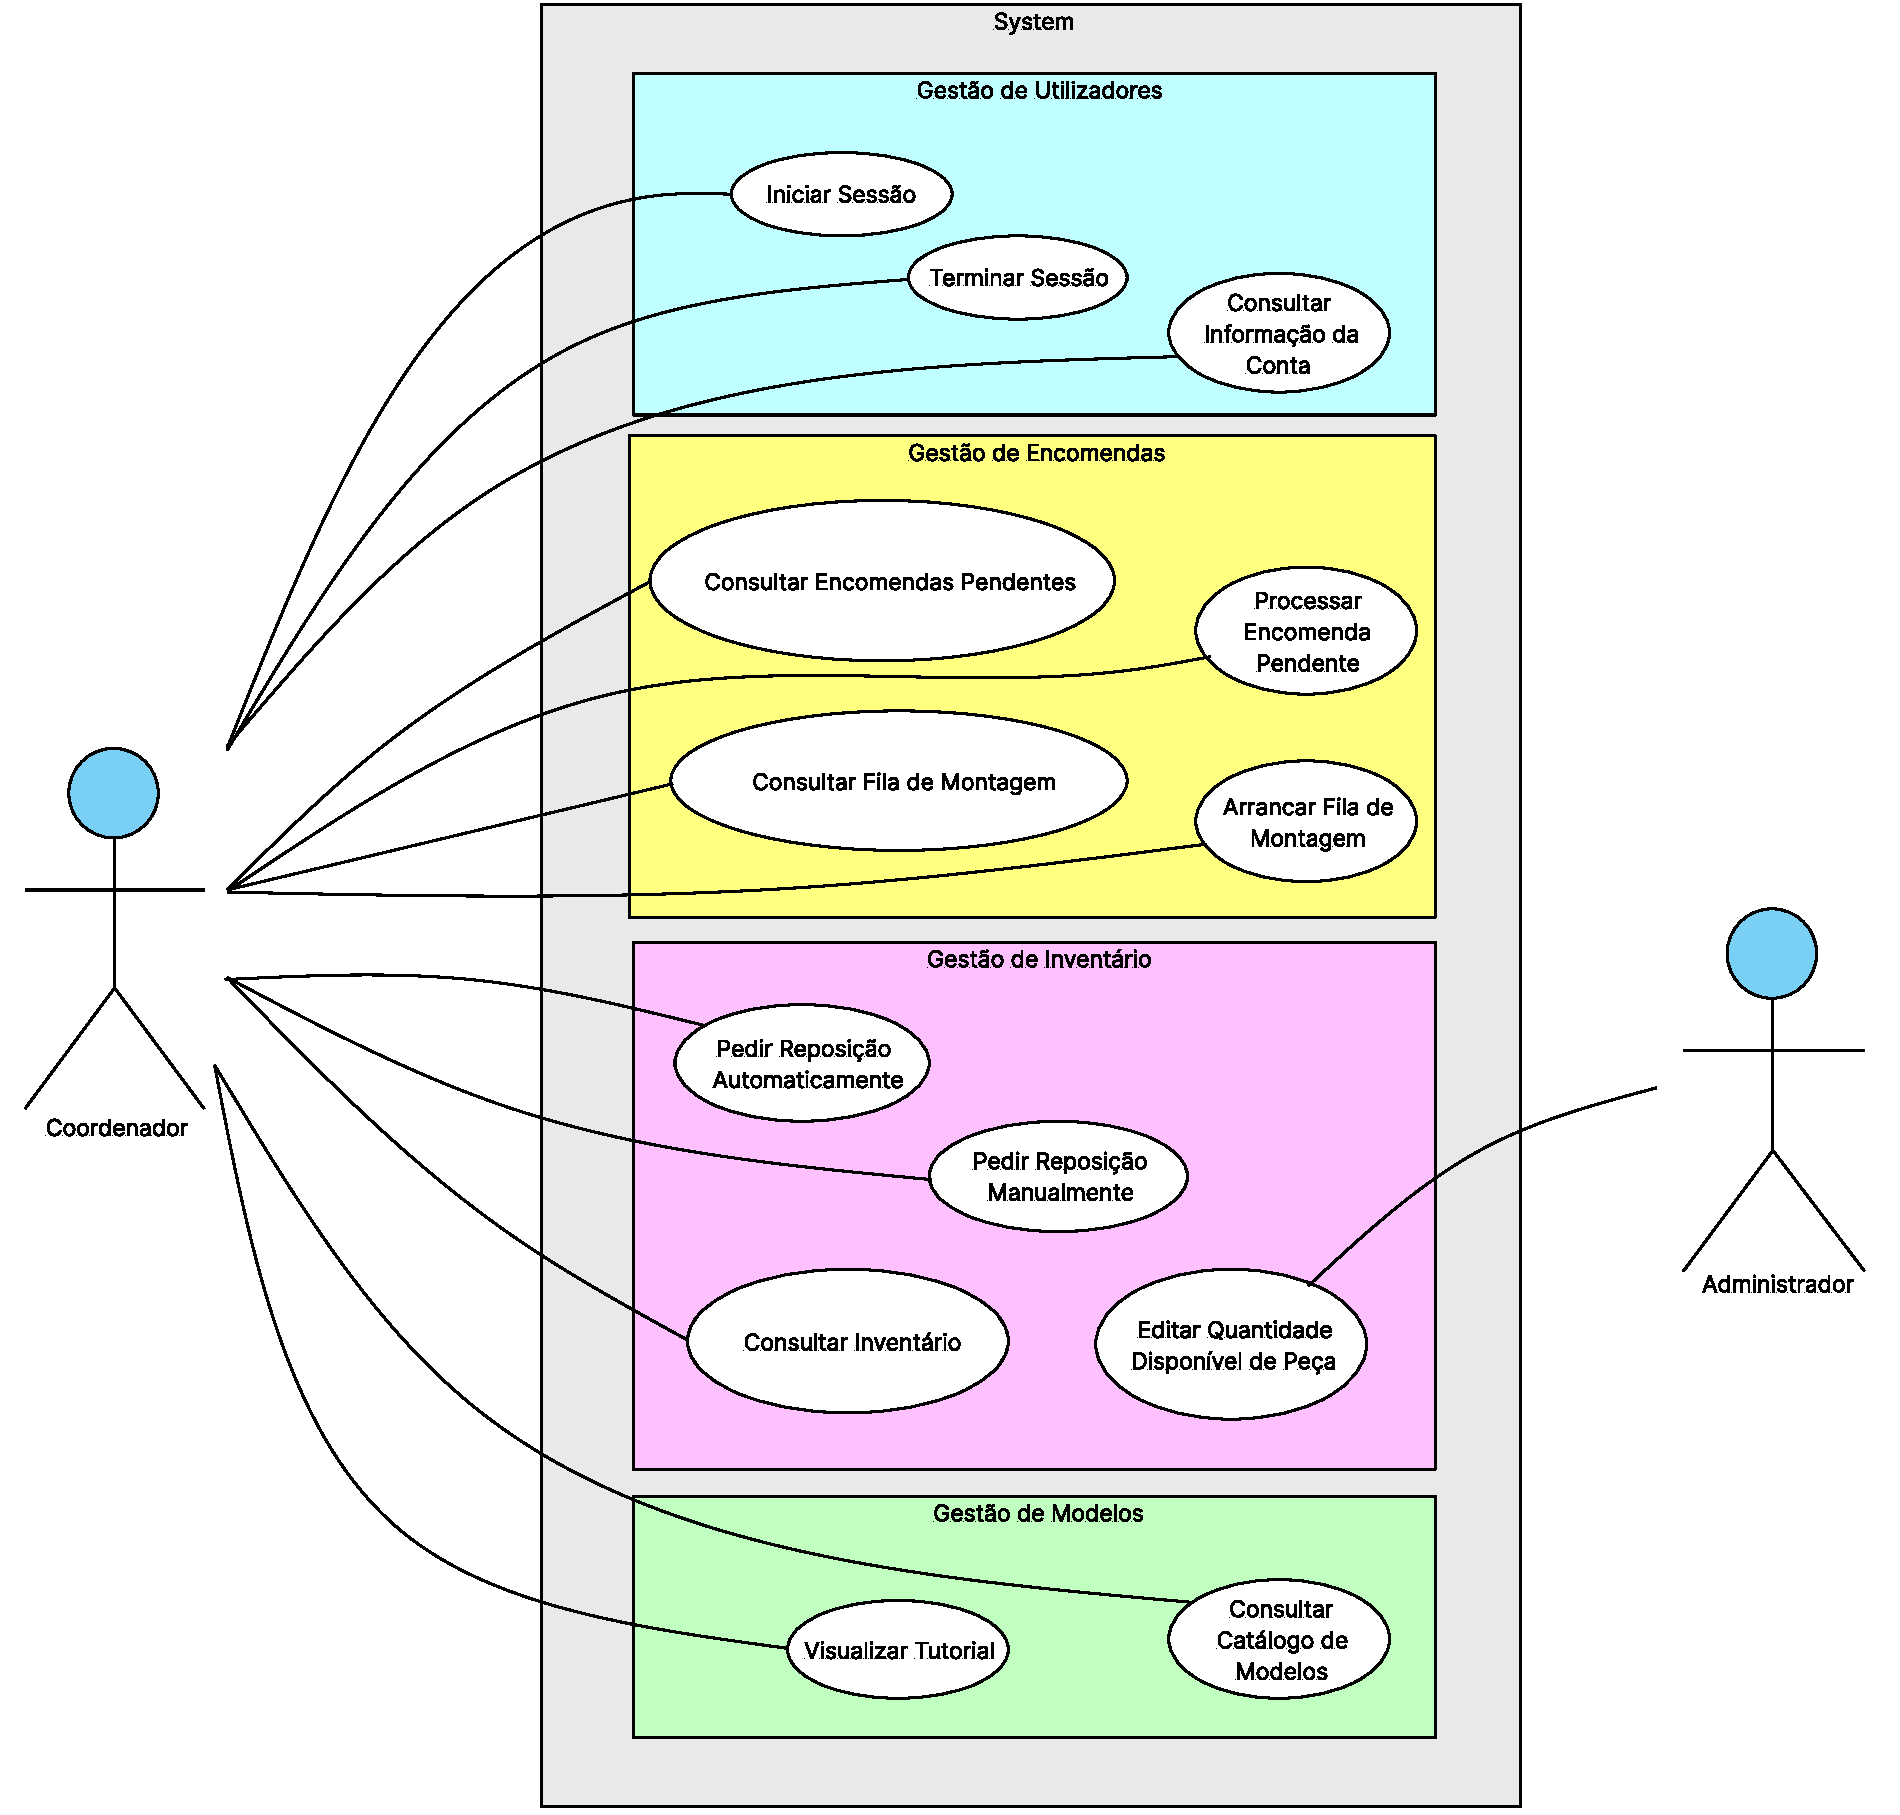
\includegraphics[width=1\textwidth]{images/cap3_diagcasos.pdf}
            \caption{Diagrama de casos de uso}
            \label{fig:diagcasos}
        \end{figure}
        
        %%%%%%%%%%%%%%%%%%%%%%%%%%%%%%%%%%%%%%%%%%%%%%%%%%%%%%%%%%%%%%%%%%%%%%%%%%%%%%%            
        %%%%%%%%%%%%%%%%%%%%%%%%%%%%%%%%%%%%%%%%%%%%%%%%%%%%%%%%%%%%%%%%%%%%%%%%%%%%%%%
        \newpage
        \subsection{Casos de Uso sobre Encomendas}

            \headercaso{Consultar Encomendas Pendentes}
                {O Coordenador consulta as encomendas pendentes para saber quais são viáveis para conceção.}
                {Utilizador tem sessão iniciada.}
                {Encomendas pendentes são amostradas no ecrã.}

            \normal{Fluxo Normal}
            {
                Utilizador acede às encomendas pendentes,
                Sistema carrega registos das encomendas pendentes,
                Sistema calcula peças em falta para cada encomenda segundo inventário,
                Sistema apresenta encomendas pendentes
            }

            \alt{Fluxo de Exceção 1 (sem encomendas pendentes)}{2}
            {
                Sistema informa não ter encomendas pendentes
            }

            %%%%%%%%%%%%%%%%%%%%%%%%%%%%%%%%%%%%%%%%%%%%%%%%%%%%%%%%%%%%%%%%%%%%%%%%%%%
            \newpage
            \headercaso{Processar Encomenda Pendente}
                {O Coordenador processa uma encomenda para adicioná-la à fila de montagem - se for viável, i.e. se houver peças disponíveis no inventário para conceber todos os seus modelos inclusos.}
                {Encomenda encontra-se em estado "pendente".}
                {Encomenda encontra-se em estado "em fila".}

            \normal{Fluxo Normal}
            {
                Utilizador seleciona encomenda pendente a processar,
                Sistema subtrai do inventário as peças necessárias à encomenda,
                Sistema edita estado da encomenda de "pendente" para "em fila"
            }

            \alt{Fluxo Exceção 1 (encomenda é inviável, faltam peças)}{1}
            {
                Sistema pergunta se rejeita a encomenda ou gera um pedido automático de restock,
                Utilizador escolhe rejeitar a encomenda,
                Sistema atualiza estado da encomenda de "pendente" para "rejeitada"
            }

            \alt{Fluxo Exceção 2 (escolhe gerar pedido de reposição automático)}{2.2}
            {
               \textit{«include» caso "Pedir Reposição Automaticamente"}
            }

            %%%%%%%%%%%%%%%%%%%%%%%%%%%%%%%%%%%%%%%%%%%%%%%%%%%%%%%%%%%%%%%%%%%%%%%%%%%
            \newpage
            \headercaso{Arrancar Fila de Montagem}
                {O Coordenador arranca a montagem das encomendas presentes na fila para serem montadas.}
                {Existem encomendas com estado "em fila".}
                {Encomendas de estado "em fila" passam a estado "finalizada".}

            \normal{Fluxo Normal}
            {
                Utilizador solicita arranque da montagem das encomendas em fila,
                Sistema carrega encomenda à frente da fila,
                Sistema apresenta sequência de passos de modelo não finalizado,
                Utilizador observa todos os passos de montagem até ao último,
                Sistema solicita confirmação de montagem do modelo,
                Utilizador confirma,
                Sistema regista montagem do modelo na respetiva encomenda,
                Sistema verifica que encomenda atual não tem mais modelos por montar,
                Sistema atualiza estado da encomenda para "finalizada",
                Sistema verifica que não há mais encomendas na fila,
                Sistema volta ao painel principal
            }

            \alt{Fluxo Alternativo 1 (encomenda ainda tem modelos por montar)}{8}
            {
                \textit{saltar para passo 3}
            }

            \alt{Fluxo Alternativo 2 (fila ainda tem encomendas)}{10}
            {
               \textit{saltar para passo 2}
            }
        %%%%%%%%%%%%%%%%%%%%%%%%%%%%%%%%%%%%%%%%%%%%%%%%%%%%%%%%%%%%%%%%%%%%%%%%%%%%%%%            
        %%%%%%%%%%%%%%%%%%%%%%%%%%%%%%%%%%%%%%%%%%%%%%%%%%%%%%%%%%%%%%%%%%%%%%%%%%%%%%%            
        \newpage
        \subsection{Casos de Uso sobre Inventário}
            
            \headercaso{Pedir Reposição Manualmente}
                {O Utilizador efetua, manualmente, um pedido de reposição de modo a obter essas peças no inventário mais tarde.}
                {O utilizador tem sessão iniciada.}
                {O pedido de reposição é registado.}

            \normal{Fluxo Normal}
            {   
                Sistema solicita uma nova peça para acrescentar ao carrinho,
                Utilizador indica a peça pretendida especificando cor e quantidade,
                Sistema pergunta se pretende adicionar mais peças ou concluir pedido,
                Utilizador escolhe concluir pedido,
                Sistema regista o pedido
            }

            \alt{Fluxo Alternativo 1 (utilizador escolhe adicionar mais peças)}{4}
            {
                Utilizador escolhe adicionar mais peças,
                \textit{saltar para passo 1}
            }

            %%%%%%%%%%%%%%%%%%%%%%%%%%%%%%%%%%%%%%%%%%%%%%%%%%%%%%%%%%%%%%%%%%%%%%%%%%%
            \newpage
            \headercaso{Pedir Reposição Automaticamente}
                {O utilizador decide colmatar uma encomenda inviável gerando um pedido automático de reposição das peças que lhe faltam.}
                {O utilizador tenta processar uma encomenda inviável.}
                {O pedido de reposição é registado.}

            \normal{Fluxo Normal}
            {
                Utilizador seleciona encomenda pendente inviável,
                Sistema apresenta uma lista de todas as peças que o pedido automático incluirá,
                Sistema solicita confirmação do utilizador,
                Utilizador confirma o pedido,
                Sistema regista o pedido
            }

            %%%%%%%%%%%%%%%%%%%%%%%%%%%%%%%%%%%%%%%%%%%%%%%%%%%%%%%%%%%%%%%%%%%%%%%%%%%
            \newpage
            \headercaso{(Administrativo) Editar Quantidade Disponível de Peça}
                {O administrador edita a quantidade de certa peça no inventário.}
                {O utilizador iniciou sessão.}
                {A quantidade especificada é atribuída à peça pretendida.}

            \normal{Fluxo Normal}
            {
                Utilizador indica uma peça no inventário para editar quantidade disponível,
                Sistema solicita senha de administrador,
                Utilizador introduz senha de administrador,
                Sistema testa corretidão da senha introduzida,
                Sistema conclui que senha está certa,
                Sistema solicita a nova quantidade,
                Utilizador introduz quantidade,
                Sistema atualiza registo de quantidade existente da peça em inventário
            }

            \alt{Fluxo Exceção 1 (senha está errada)}{6}
            {
                Sistema regressa à apresentação do inventário
            }
            
        %%%%%%%%%%%%%%%%%%%%%%%%%%%%%%%%%%%%%%%%%%%%%%%%%%%%%%%%%%%%%%%%%%%%%%%%%%%%%%%            
        %%%%%%%%%%%%%%%%%%%%%%%%%%%%%%%%%%%%%%%%%%%%%%%%%%%%%%%%%%%%%%%%%%%%%%%%%%%%%%%            
        \newpage        
        \subsection{Casos de Uso sobre Modelos}

            \headercaso{Consultar Catálogo de Modelos}
                {O coordenador consulta, de forma desenquadrada da montagem, o catálogo de modelos que o sistema reconhece.}
                {Utilizador está autenticado.}
                {Utilizador consegue observar uma listagem dos modelos registados no sistema.}

            \normal{Fluxo Normal}
            {
                Utilizador acede ao catálogo de modelos,
                Sistema carrega registos a respeito dos modelos,
                Sistema apresenta uma listagem dos modelos existentes incluindo as peças requeridas por cada
            }       
            
            %%%%%%%%%%%%%%%%%%%%%%%%%%%%%%%%%%%%%%%%%%%%%%%%%%%%%%%%%%%%%%%%%%%%%%%%%%%
            \newpage
            \headercaso{Visualizar Sequência de Montagem Desenquadrada}
                {O utilizador visualiza, fora do contexto da linha de montagem, a sequência de montagem dum modelo que pretenda.}
                {Sistema tem registo do modelo pretendido.}
                {Utilizador consegue observar a sequência de montagem relativa ao modelo pretendido.}

            \normal{Fluxo Normal}
            {
                Utilizador indica um modelo no catálogo cuja sequência de montagem pretenda visualizar,
                Sistema carrega e apresenta a sequência de passos de montagem do modelo
            }

%==========================================================================
% END #3 - ESPECIFICAÇAO/MODELAÇAO DO SOFTWARE
%==========================================================================
%==========================================================================
% BEGIN #4 - CONCEÇAO DO SISTEMA DE DADOS
% Descrição e caracterização geral do sistema responsável pelo armazenamento da informação requerida pelo sistema que idealizaram e especificaram.
%==========================================================================

\chapter{Conceção do Sistema de Dados}
    Os requisitos exigem acesso tanto a um catálogo de modelos e peças como a um registo de utilizadores da aplicação, que a usam para assinalar a sua autoria na conceção de encomendas. Com isto em mente, partiu-se do diagrama estrutural de domínio para estabelecer como os dados se organizam na base de dados, duma forma que minimize a interdependência mas introduzindo redundâncias úteis em nome da eficiência.
    
    \section{Estrutura do Sistema de Dados}
        Desta forma após análise dos requisitos, maquete e modelos que foram desenvolvidos para sustentar o sistema, foi criado o seguinte modelo lógico da base de dados:
        \begin{figure}
            \centering
            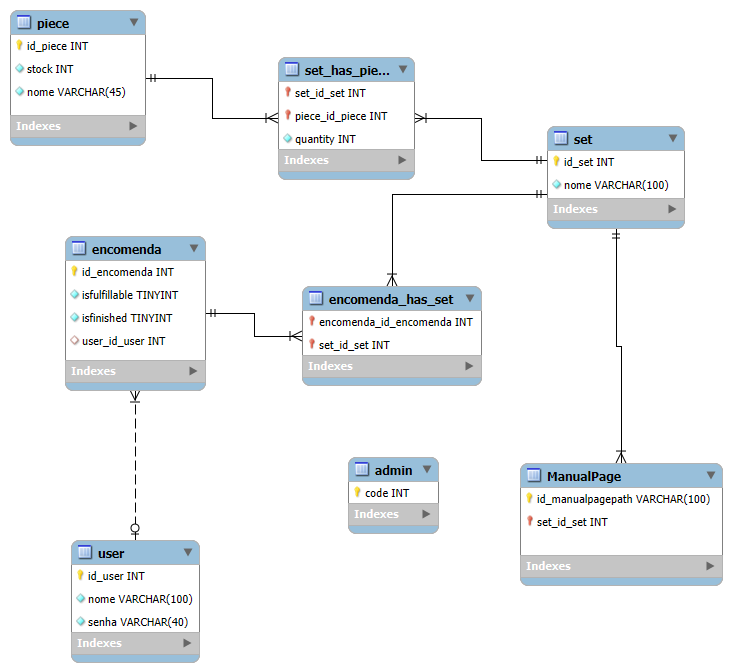
\includegraphics[width=\textwidth]{images/modelologico.png}
            \caption{Modelo lógico}
            \label{fig:modelologico}
        \end{figure}

    \newpage
    \section{Descrição de Elementos e seus Relacionamentos}
    Para melhor compreensão do modelo lógico da base de dados apresentámos duas tabelas para ajudar na perceção das entidades e relacionamentos da mesma.
    \begin{table}[h!]
    \centering
    \renewcommand{\arraystretch}{1.5} % Ajusta o espaçamento entre as linhas
    \begin{tabular}{|m{3cm}|m{6cm}|m{6cm}|}
        \hline
        \rowcolor{gray!28} % Cor de fundo da linha de cabeçalho
        \textbf{Entidade} & \textbf{Descrição} & \textbf{Ocorrência} \\ \hline
        \textbf{User} & Descrição geral para os que usam a aplicação na linha de produção & Cada user pode processar uma encomenda. \\ \hline
        \textbf{Encomenda} & Descrição geral para os pedidos vindos do departamento de gestão que contém os Sets a produzir para cada um. & Os users processam uma encomenda de cada vez, no caso produzem o Set dessa mesma encomenda. \\ \hline
        \textbf{Set} & Descrição geral para o produto que é produzido nas linhas de montagem. & Cada user vai produzir estes Sets consoante o que é pedido na encomenda. \\ \hline
        \textbf{Piece} & Descrição geral para o que compõe um Set. & O user vai usar este objeto para produzir os Sets, tendo sempre em atenção o stock do objeto. \\ \hline
        \textbf{ManualPage} & Descrição geral para uma instrução de montagem do Set. & Cada Set terá a si associado várias páginas que demonstrarão como este é produzido. \\ \hline
        \textbf{Admin} & Descrição geral para os códigos que serão usados para validar ações na aplicação que são identificadas como ações de administrador. & Cada código de administrador vai ser usado por um user identificado pela diração da empresa, para executar funções de administrador na aplicação. \\ \hline
    \end{tabular}
    \caption{Identificação das entidades}
    \label{tab:identificacao_entidades}
\end{table}
\newpage

\begin{table}[ht]
    \centering
    \begin{tabular}{|c|c|c|c|c|c|}
        \hline
        \rowcolor{gray!28}
        \textbf{Entidade} & \textbf{Multiplicidade} & \textbf{Relacionamento} & \textbf{Multiplicidade} & \textbf{Entidade} \\ \hline
        User            & 0..1                   & processa                     & N                   & Encomenda            \\ \hline
        Encomenda        & N                   & possui               & M                   & Set         \\ \hline
        Set         & N                   & possui              & M                   & Piece             \\ \hline
        Set           & 1                   & orientado              & N                   & ManualPage             \\ \hline
    \end{tabular}
    \caption{Relacionamento entre entidades}
    \label{tab:relacionamento_entidades}
\end{table}

    A entidade "Admin" não tem nenhum relacionamento, sendo assim uma tabela isolada, devido a não interagir com nenhuma outra entidade por não ser necessário. Esta entidade é apenas utilizada para armazenar as chaves de administrador no sistema, que vão ser utilizadas por certos funcionários definidos pela direção da empresa para efetuar ações de administrador na aplicação.


        

%==========================================================================
% END #4 - CONCEÇAO DO SISTEMA DE DADOS
%==========================================================================

%==========================================================================
% BEGIN #5 - ESBOÇO DOS INTERFACES DO SISTEMA
% Descrição e caracterização das diversas interfaces requeridas pelos serviços do sistema, utilizando esboços (mockups) que revelem o aspeto pretendido para cada uma das interfaces a implementar.
%==========================================================================

\chapter{Esboço dos Interfaces do Sistema}

    Em primeiro lugar, criou-se um logótipo simples de modo a poder ser utilizado nas interfaces sem criar muita poluição visual. Consiste apenas numa peça de lego com o nome da empresa.

    \begin{figure}[h!]
        \centering
        
\includegraphics[width=0.5\linewidth]{images/autobricklogo.png}
        \caption{Logótipo}
        \label{fig:Logo}
    \end{figure}

    Para além disto, escolheu-se uma palete de cores que serão utilizadas nas interfaces de forma a torná-las mais apelativas esteticamente.

        \begin{figure}[h!]
        \centering
        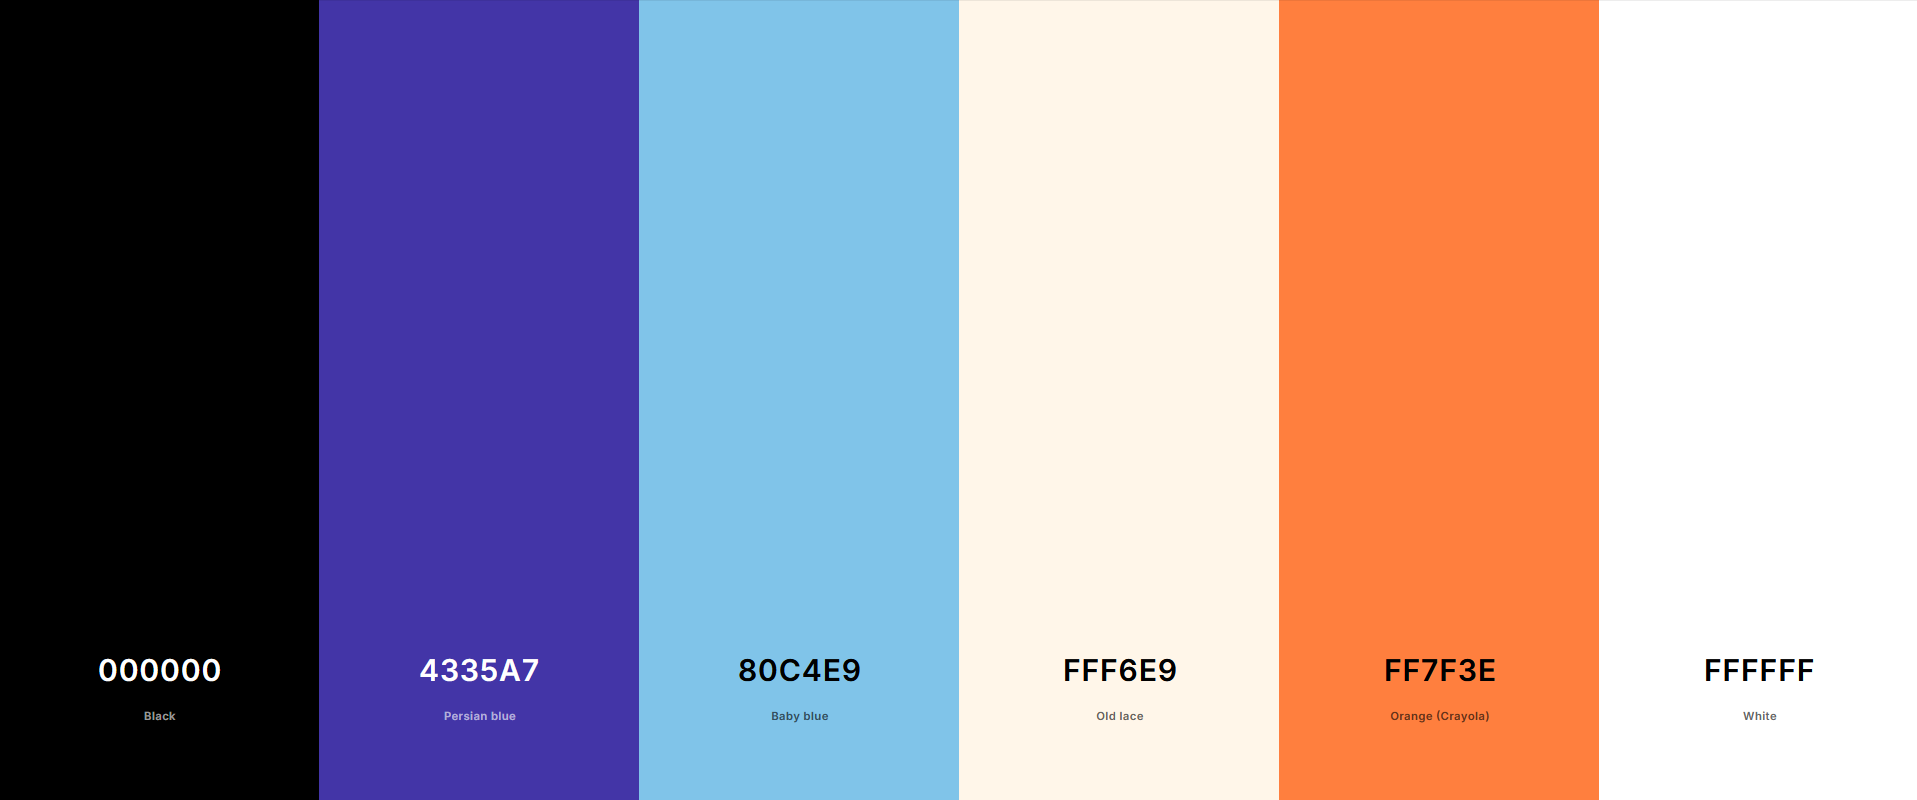
\includegraphics[width=0.8\linewidth, frame]{images/ColorPallete.png}
        \caption{Palete de cores}
        \label{fig:Palete de cores}
    \end{figure}

    Segue, assim, uma apresentação das principais interfaces.

    \clearpage
    \subsection{Interfaces de autenticação}
    
        \begin{figure}[h!]
            \centering
            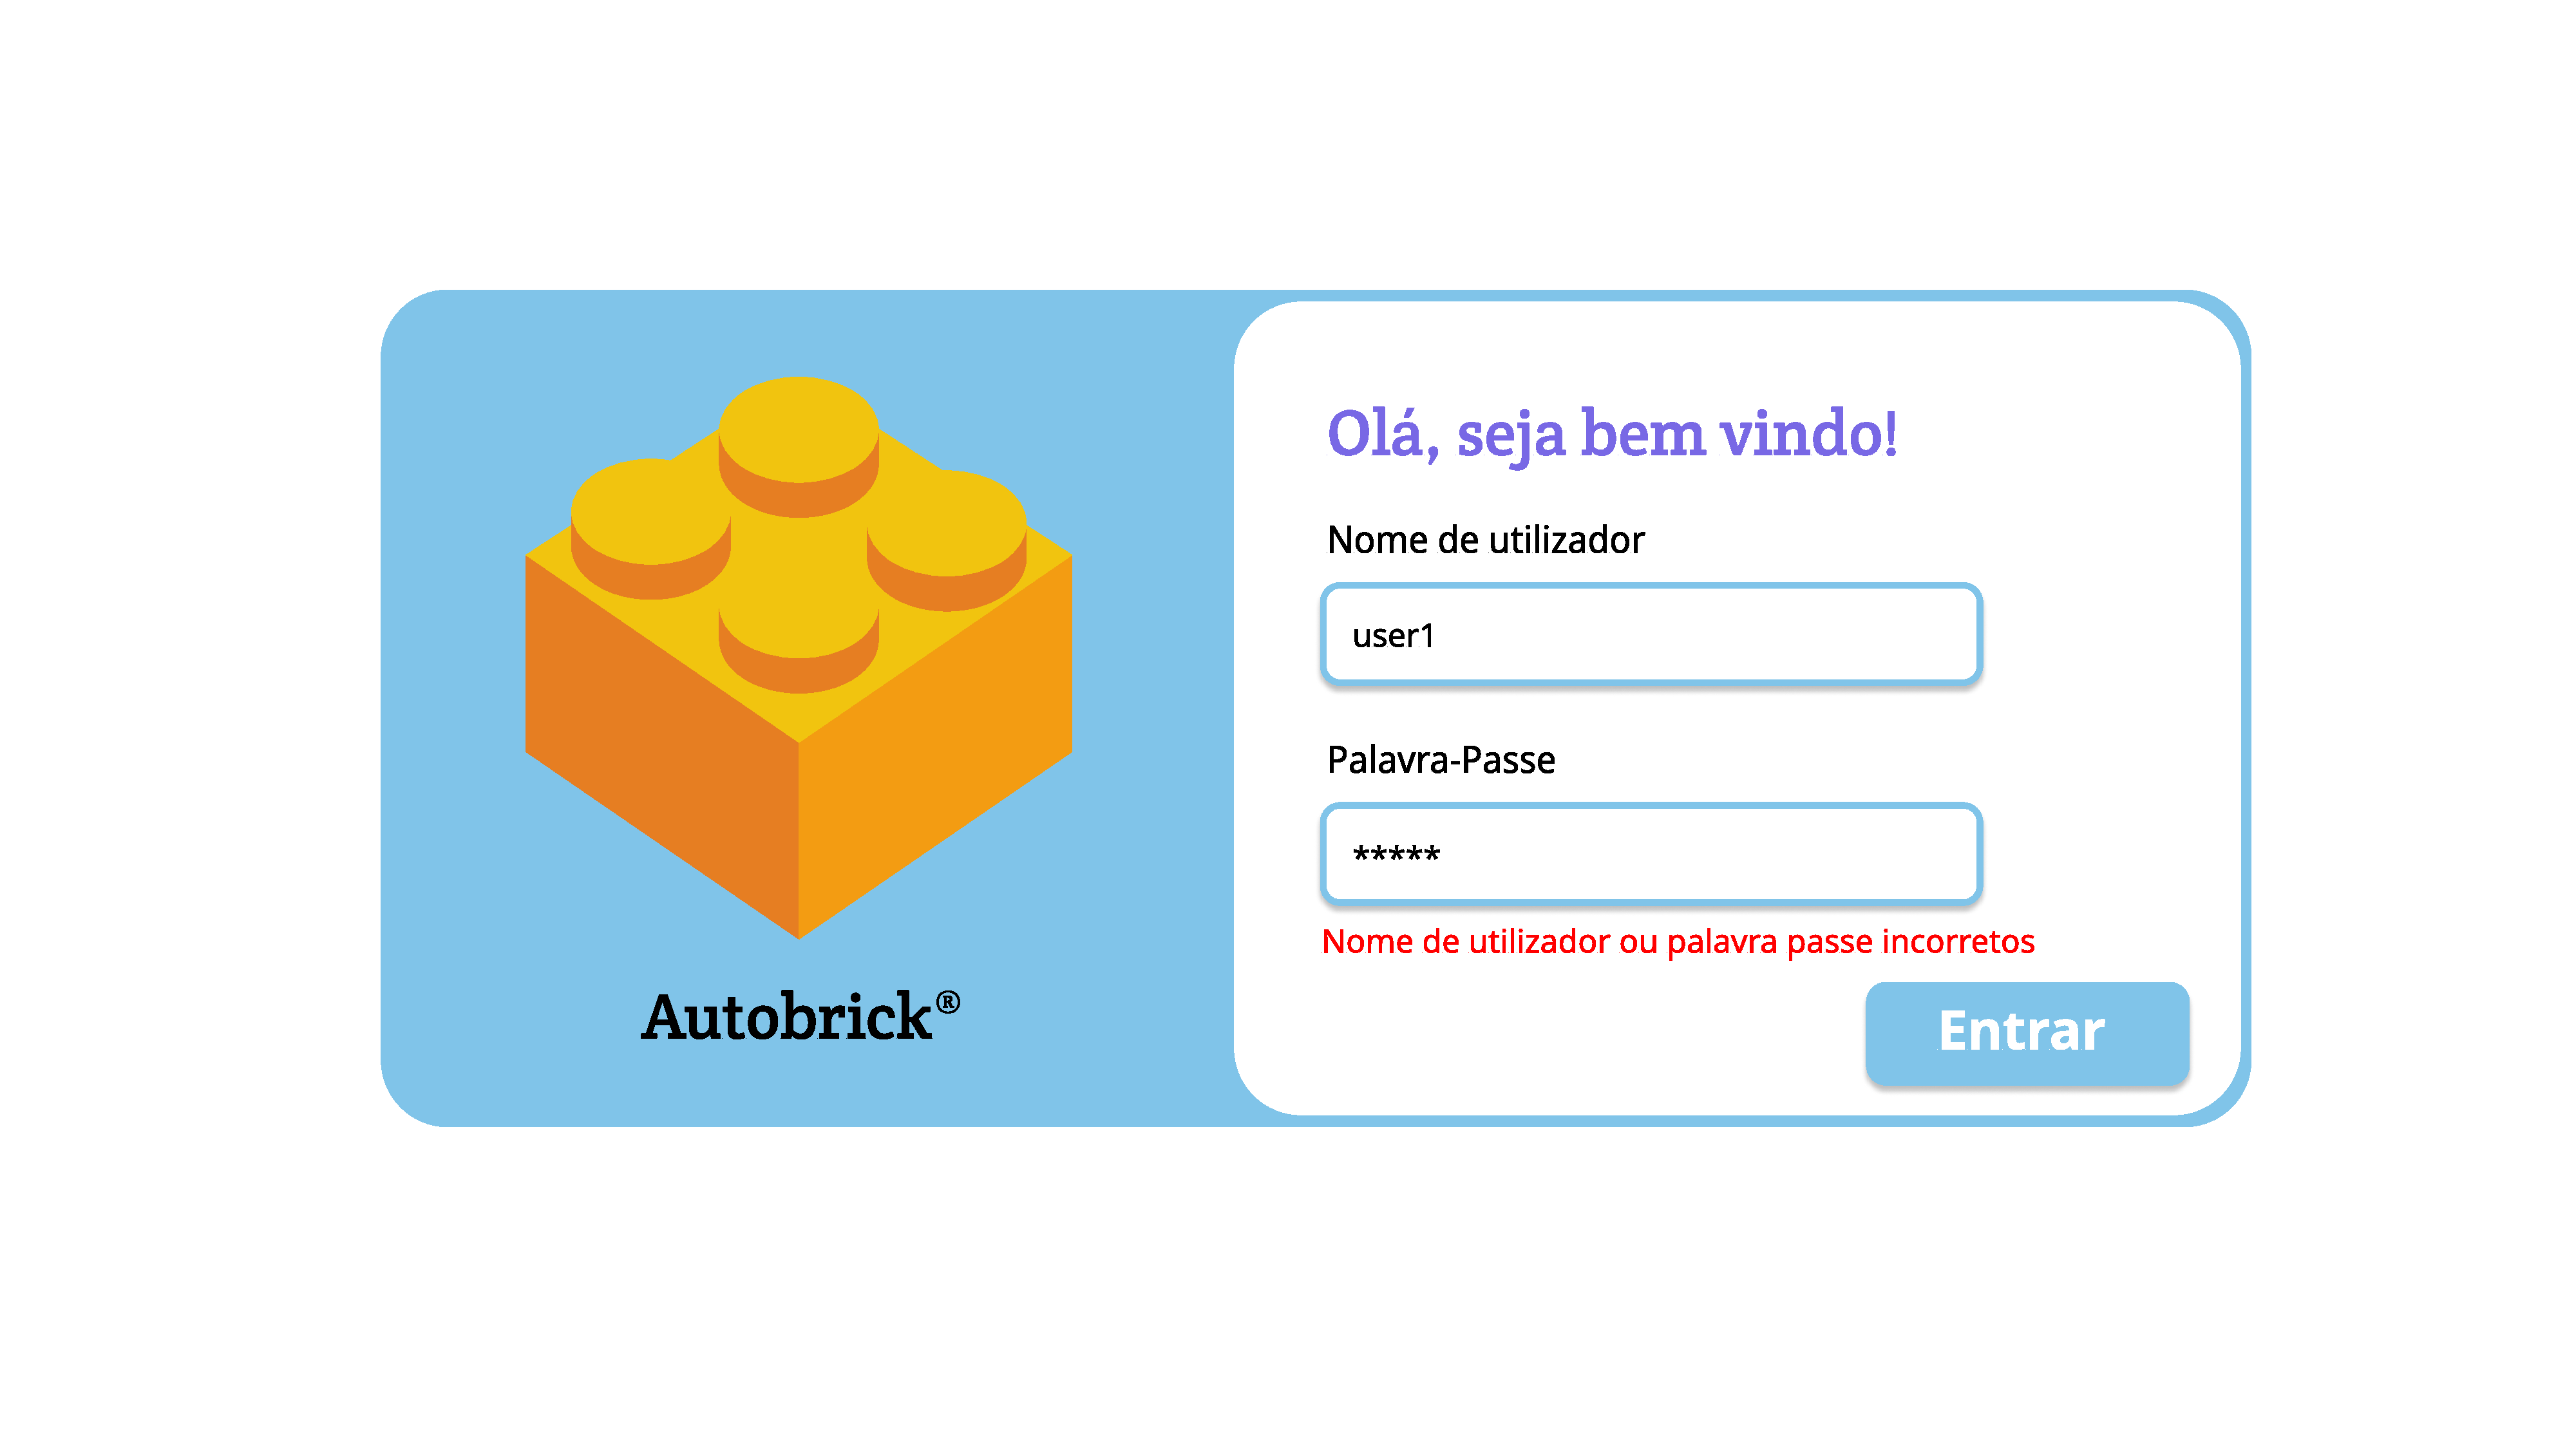
\includegraphics[width=0.99\linewidth, frame]{images/Login Failed.pdf}
            \caption{Página de Login (com credenciais erradas) }
            \label{fig:Login}
        \end{figure}
    
        Esta é a página utilizada para iniciar sessão (ver requisito 2.2.2)

        \clearpage
        \begin{figure}[h!]
            \centering
            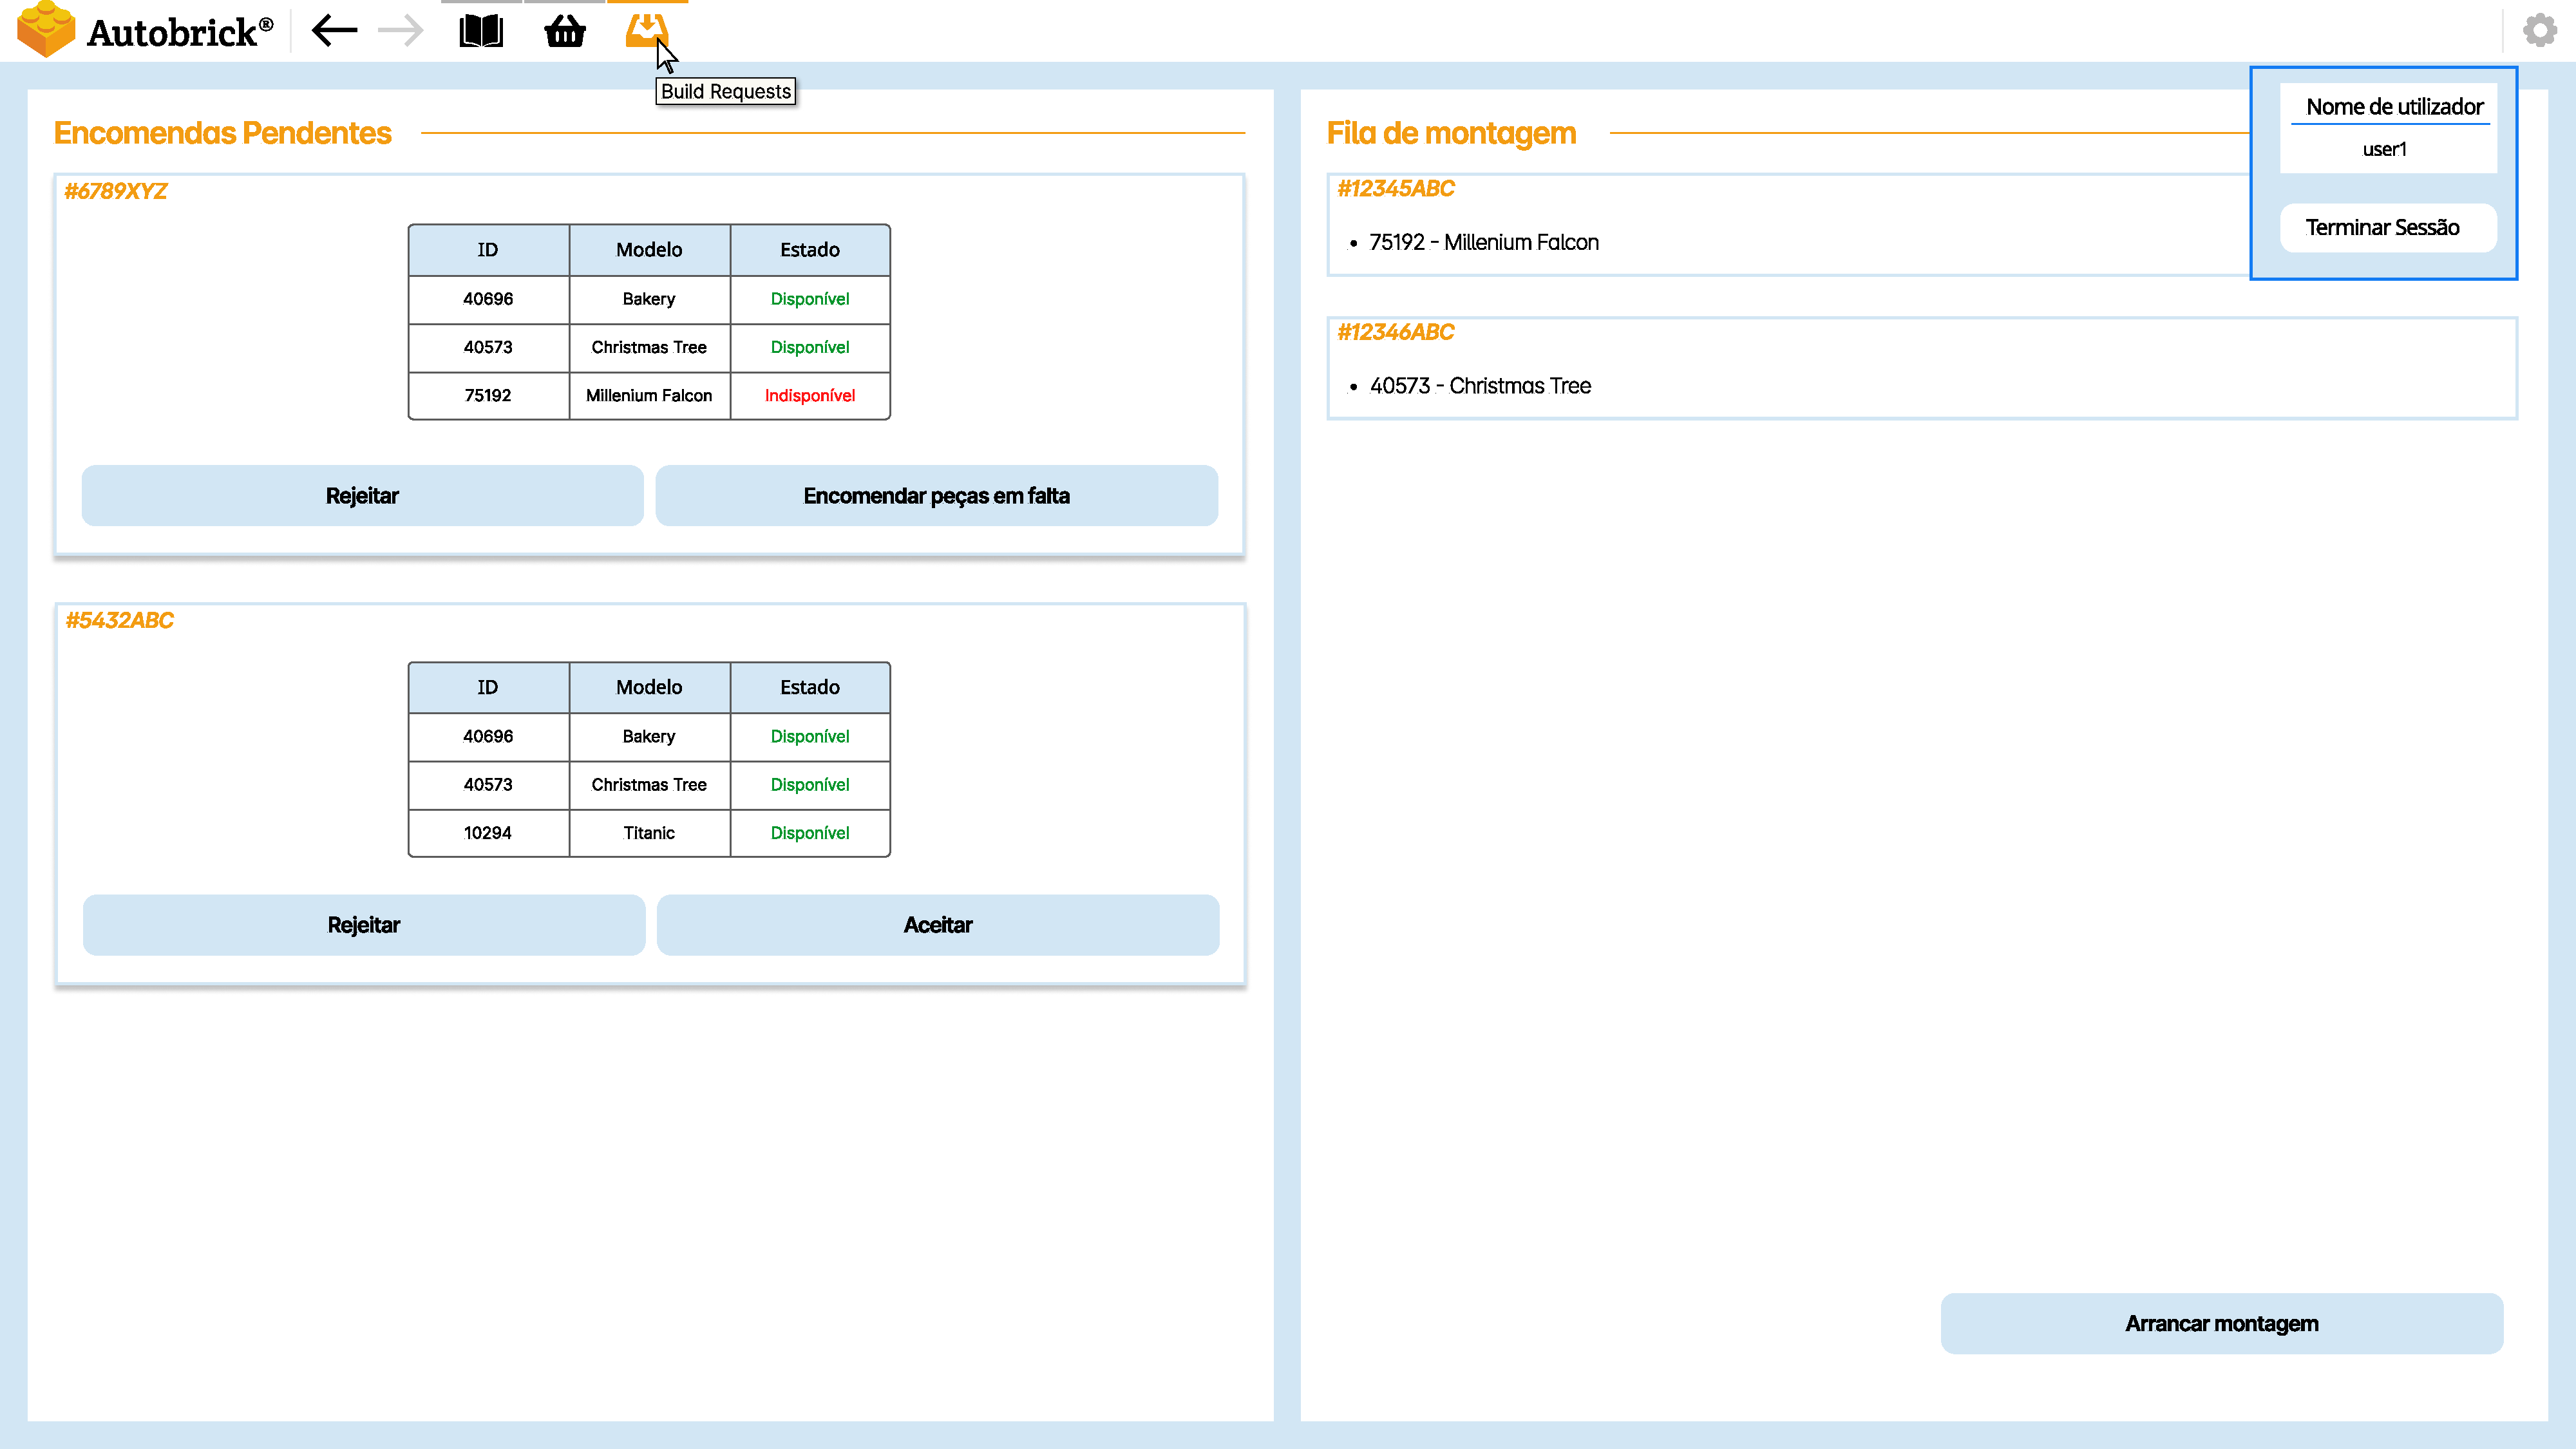
\includegraphics[width=0.99\linewidth, frame]{images/Settings.pdf}
            \caption{Página de encomendas após interação com botão de opções (engrenagem)}
            \label{fig:Settings}
        \end{figure}
        
        Quando o utilizador clica na engrenagem no canto superior direito da página, aparece um menu que lhe mostra o seu nome de utilizador (ver requisito 2.2.4) e um botão para terminar sessão (ver requisito 2.2.3).
    
        \clearpage
        \begin{figure}[h!]
            \centering
            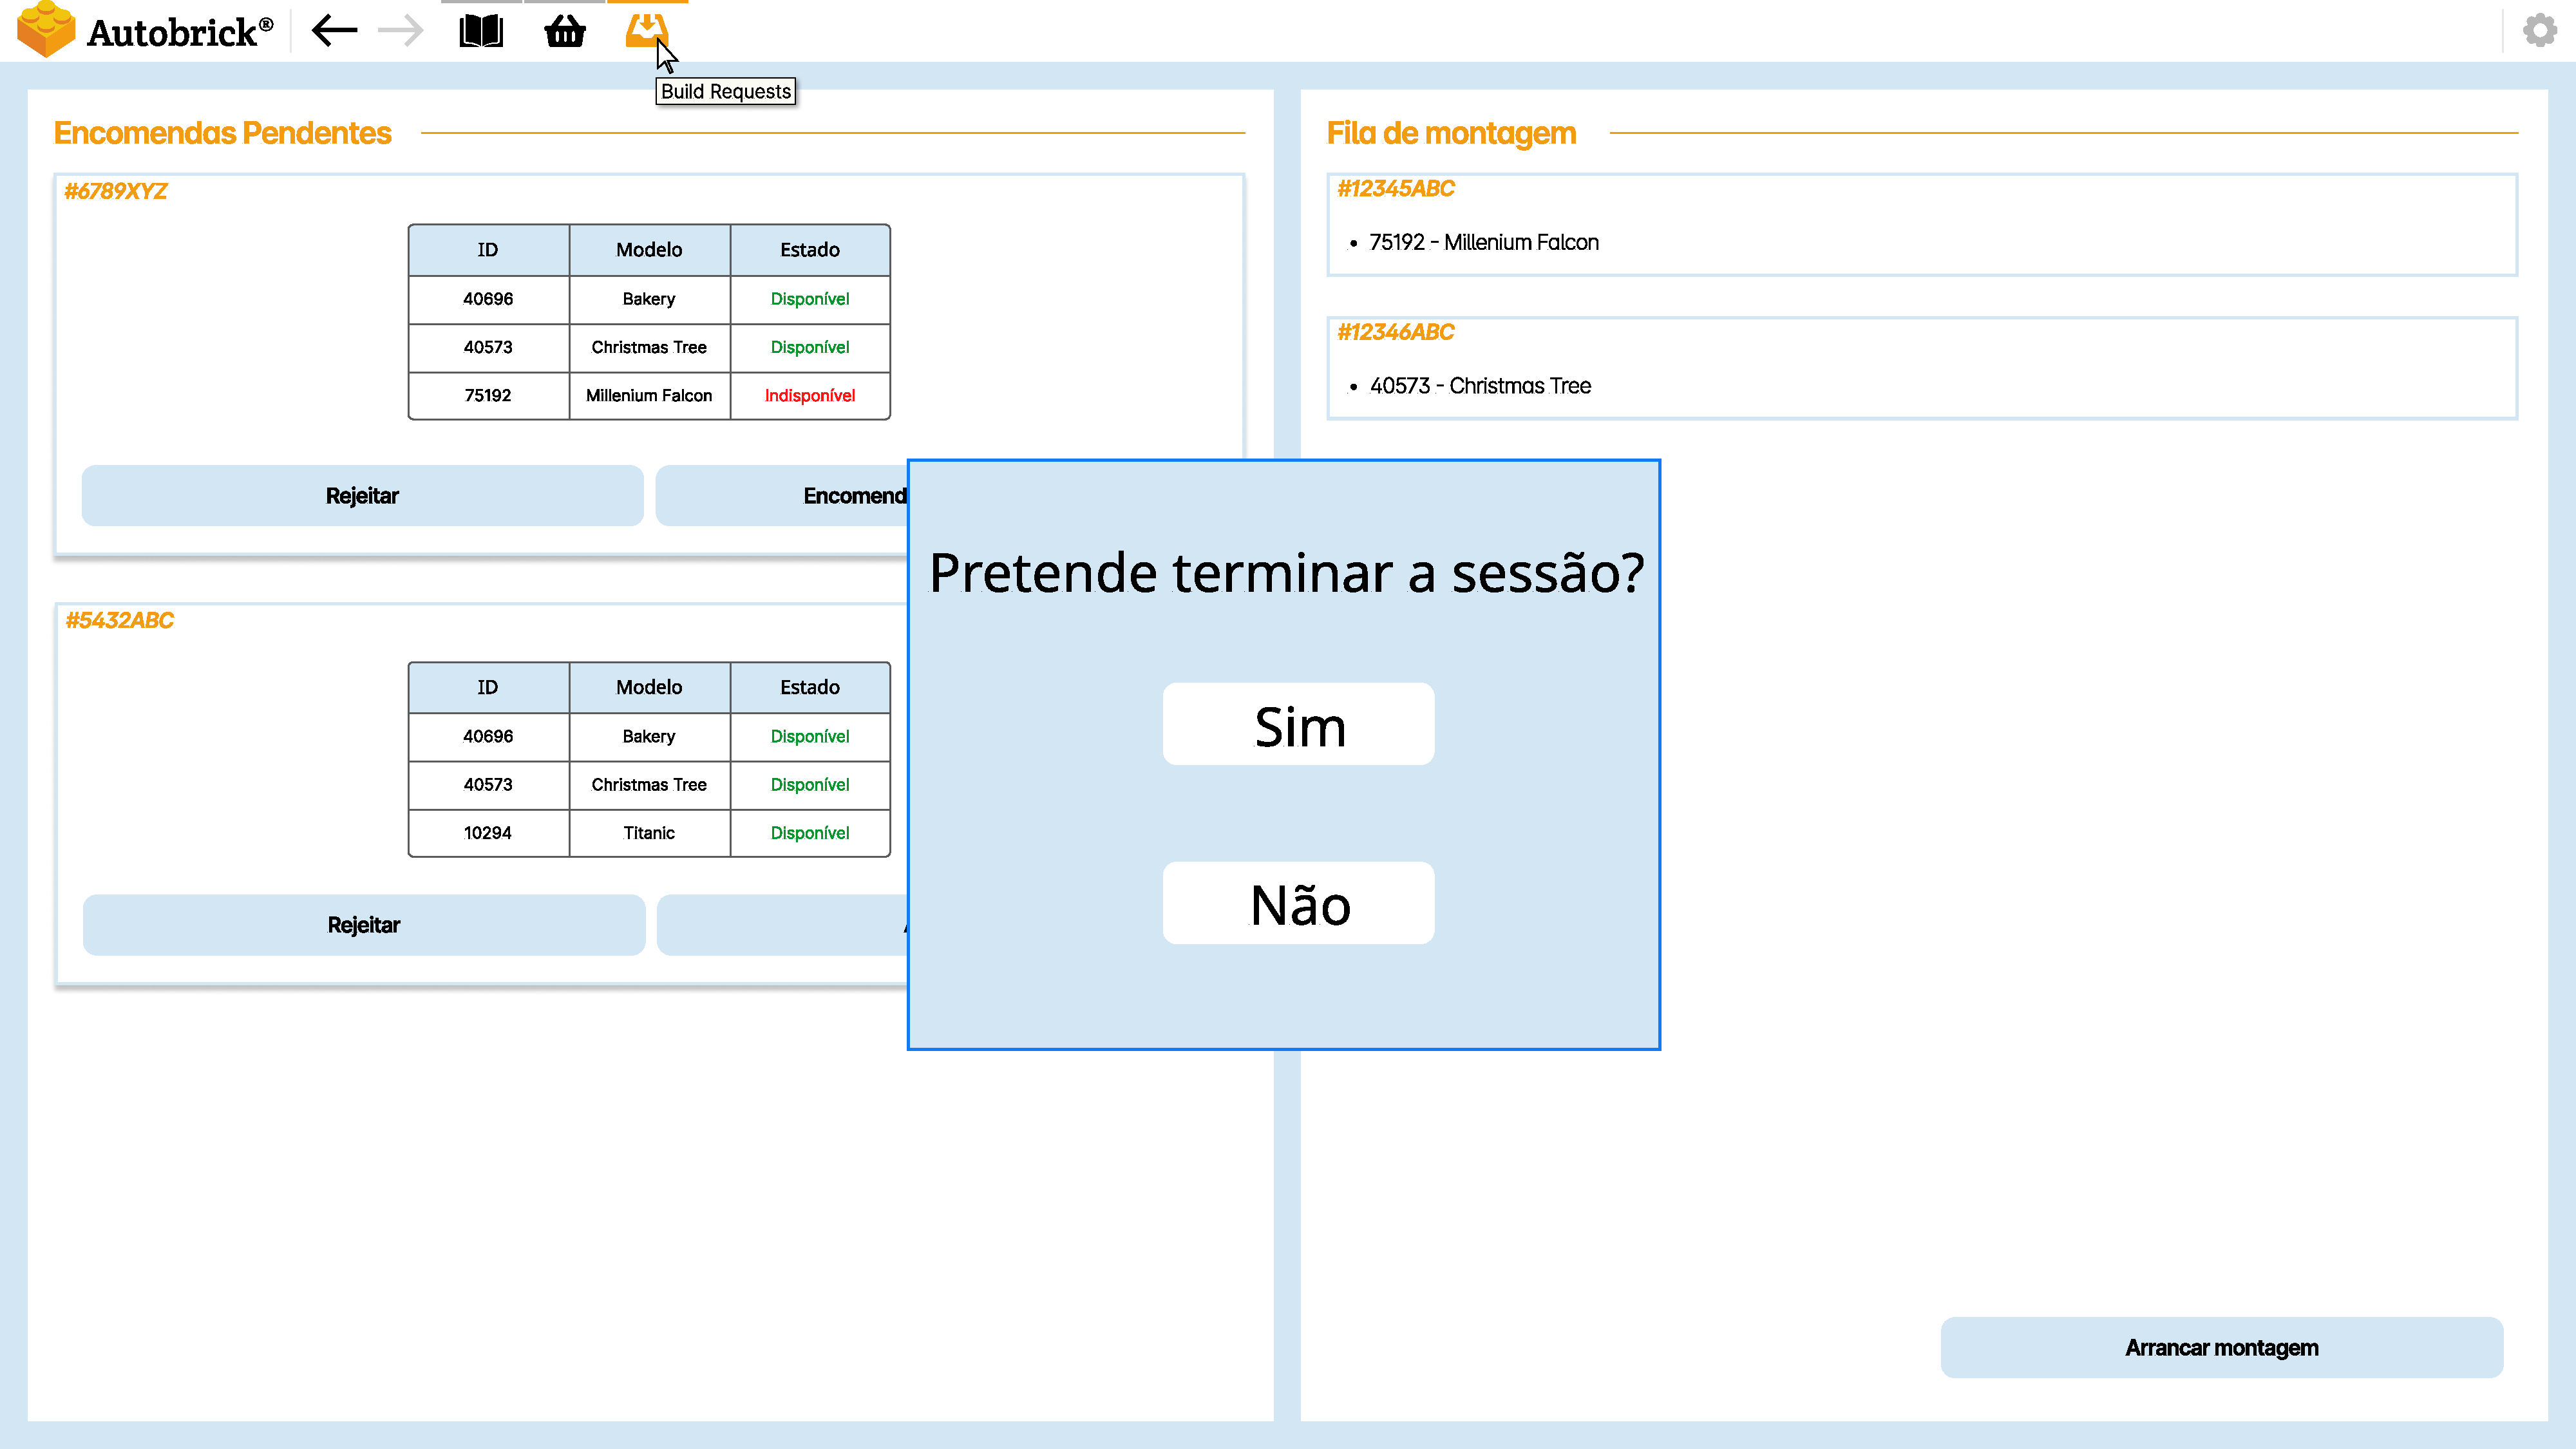
\includegraphics[width=0.99\linewidth, frame]{images/Logout.pdf}
            \caption{Página de encomendas após interação com botão de terminar sessão}
            \label{fig:Logout}
        \end{figure}
    
        Quando o utilizador carrega no botão de terminar sessão, o menu da Figura~\ref{fig:Logout} aparece para este confirmar a ação.
    
    \clearpage
    \subsection{Interfaces de Encomendas}

        \begin{figure}[h!]
            \centering
            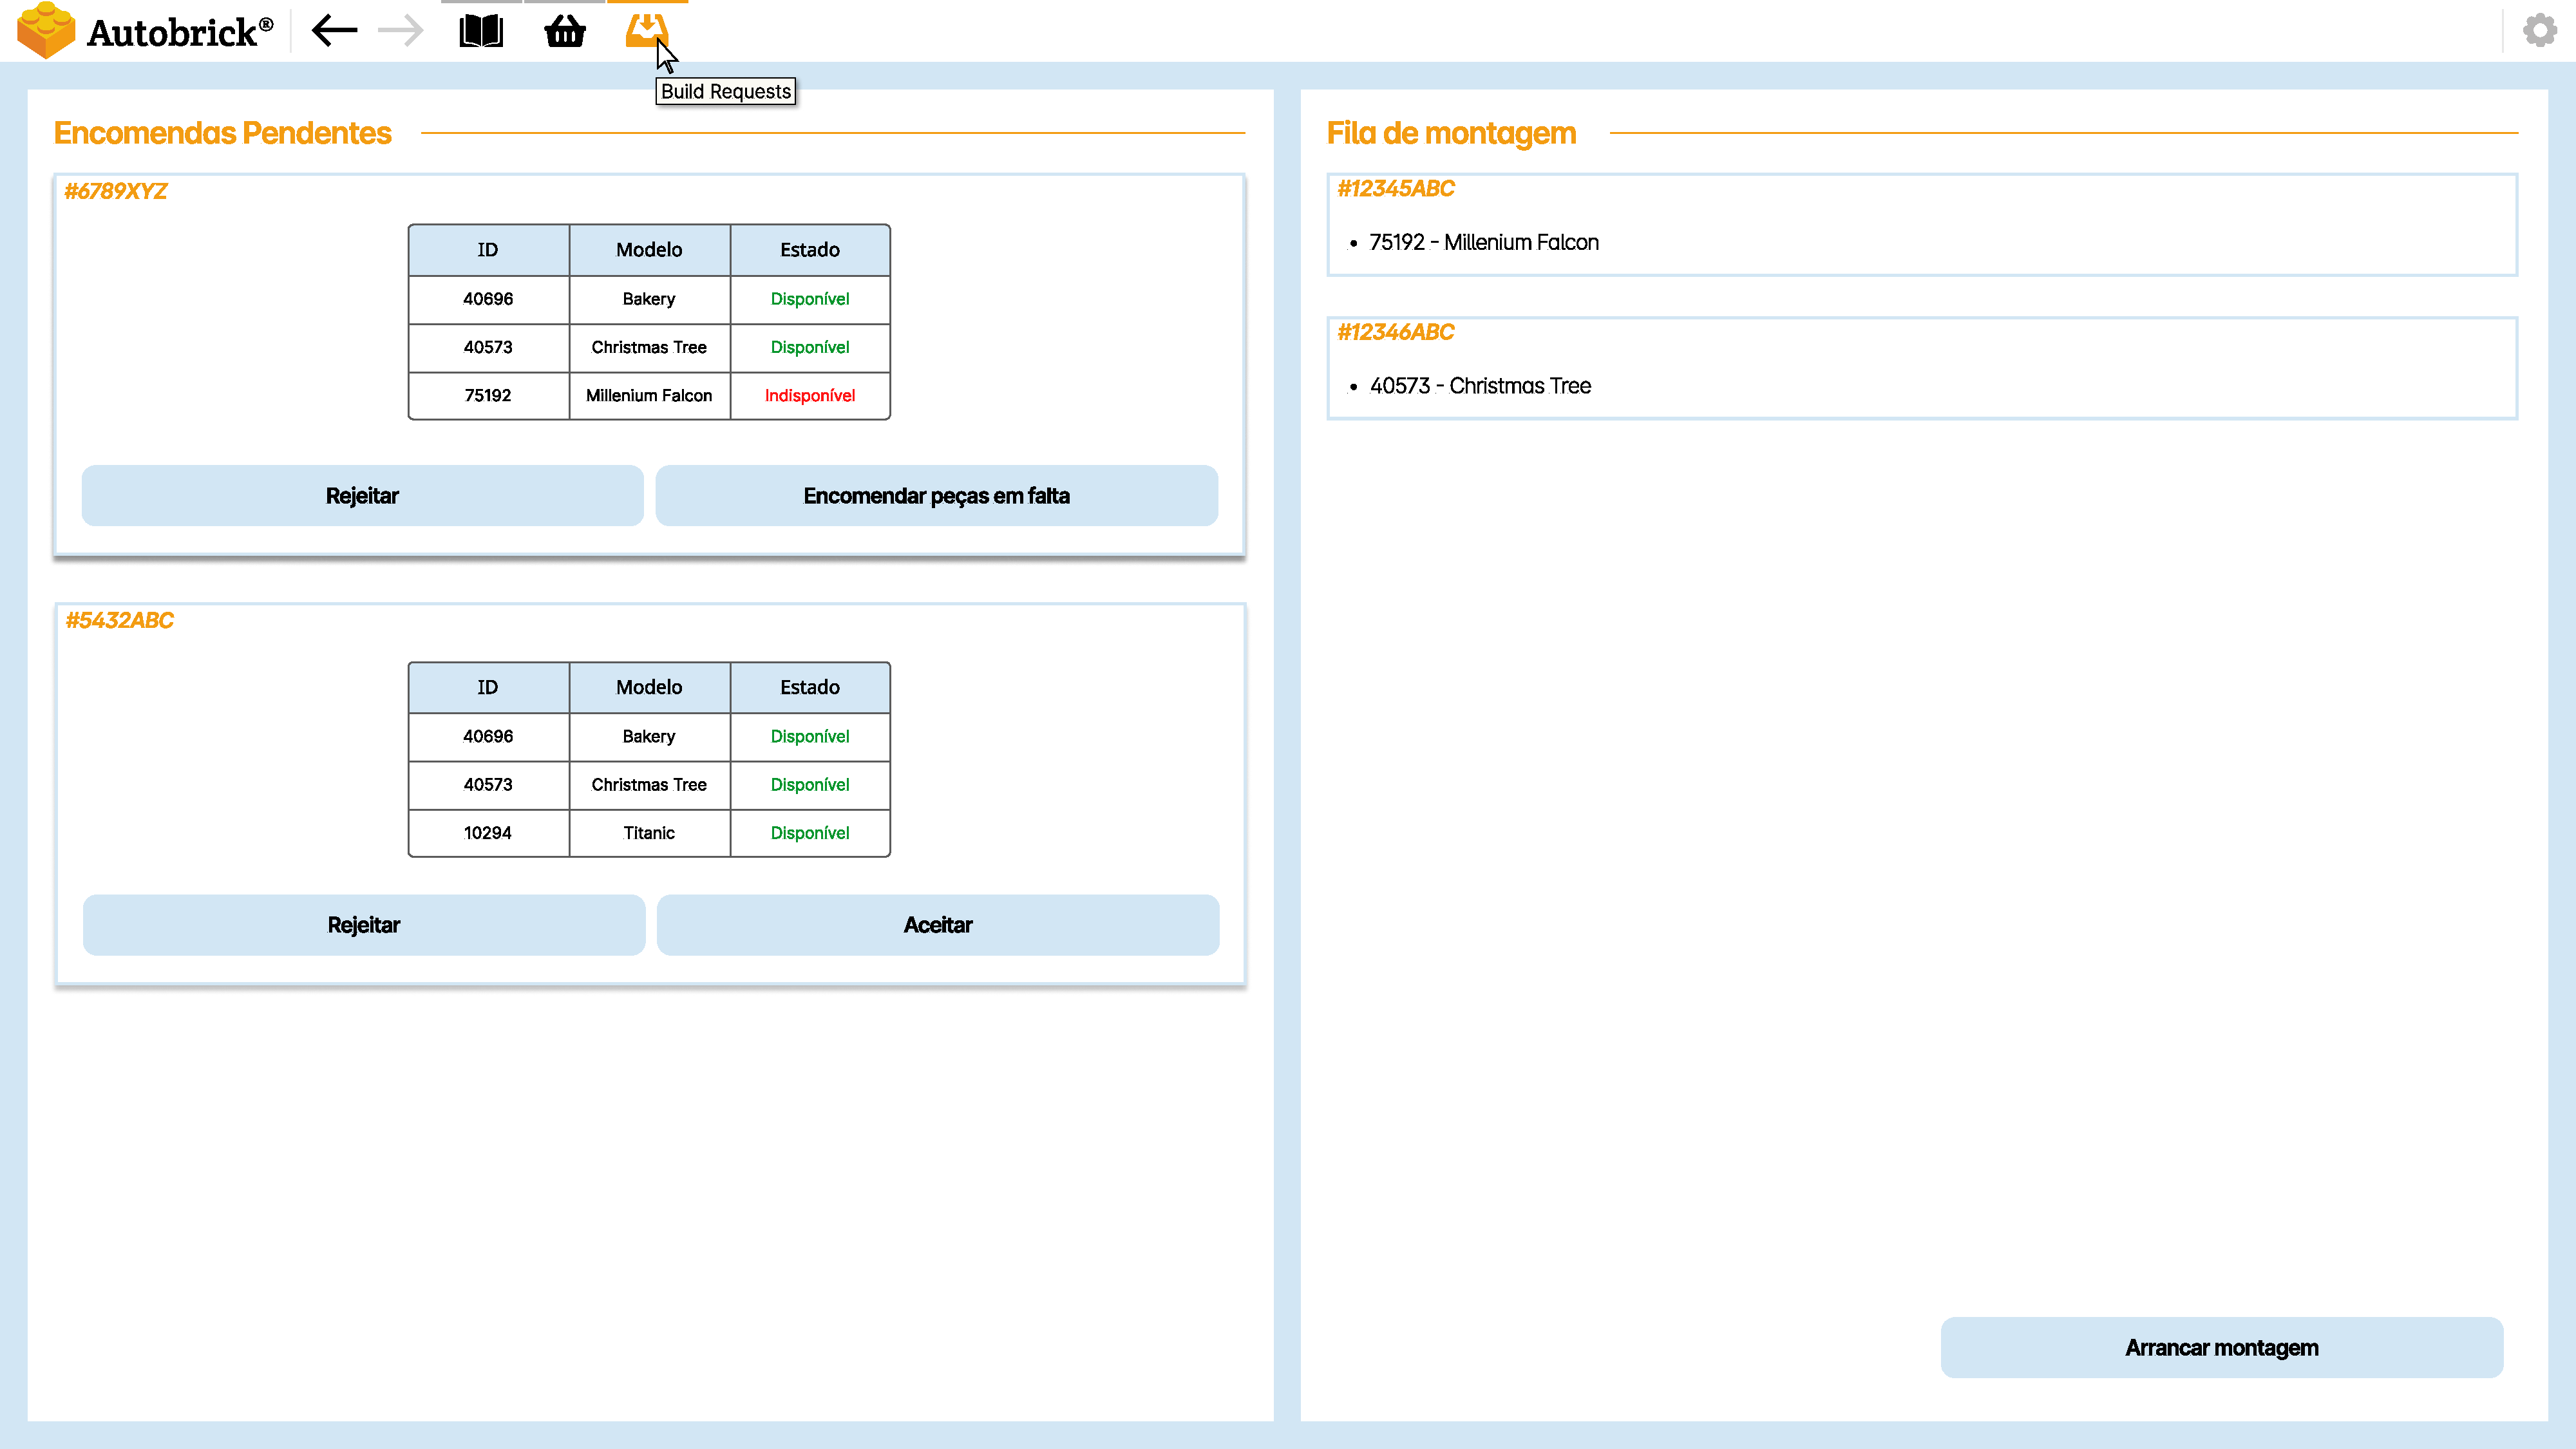
\includegraphics[width=0.85\linewidth, frame]{images/Requests.pdf}
            \caption{Página de encomendas}
            \label{fig:Encomendas}
        \end{figure}
    
        Esta é considerada a páginal principal da aplicação onde é possível iniciar a montagem da próxima encomenda na fila de montagem (ver use case 3.3.1.3), consultar encomendas pendentes (use case 3.3.1.1) bem como rejeitar ou aceitar as mesmas (ver use case 3.3.1.2). Para além disso é ainda possível encomendar as peças em falta para realizar um dado modelo (ver use case 3.3.1.2 e 3.3.2.2)
    
    
        \begin{figure}[h!]
            \centering
            \includegraphics[width=0.85\linewidth, frame]{images/Encomenda Automática.pdf}
            \caption{Página de encomendas após interação com botão de encomendar peças em falta}
            \label{fig:EncomendasAuto}
        \end{figure}
        
    \clearpage
    \subsection{Interfaces de Inventário}
    
        \begin{figure}[h!]
            \centering
            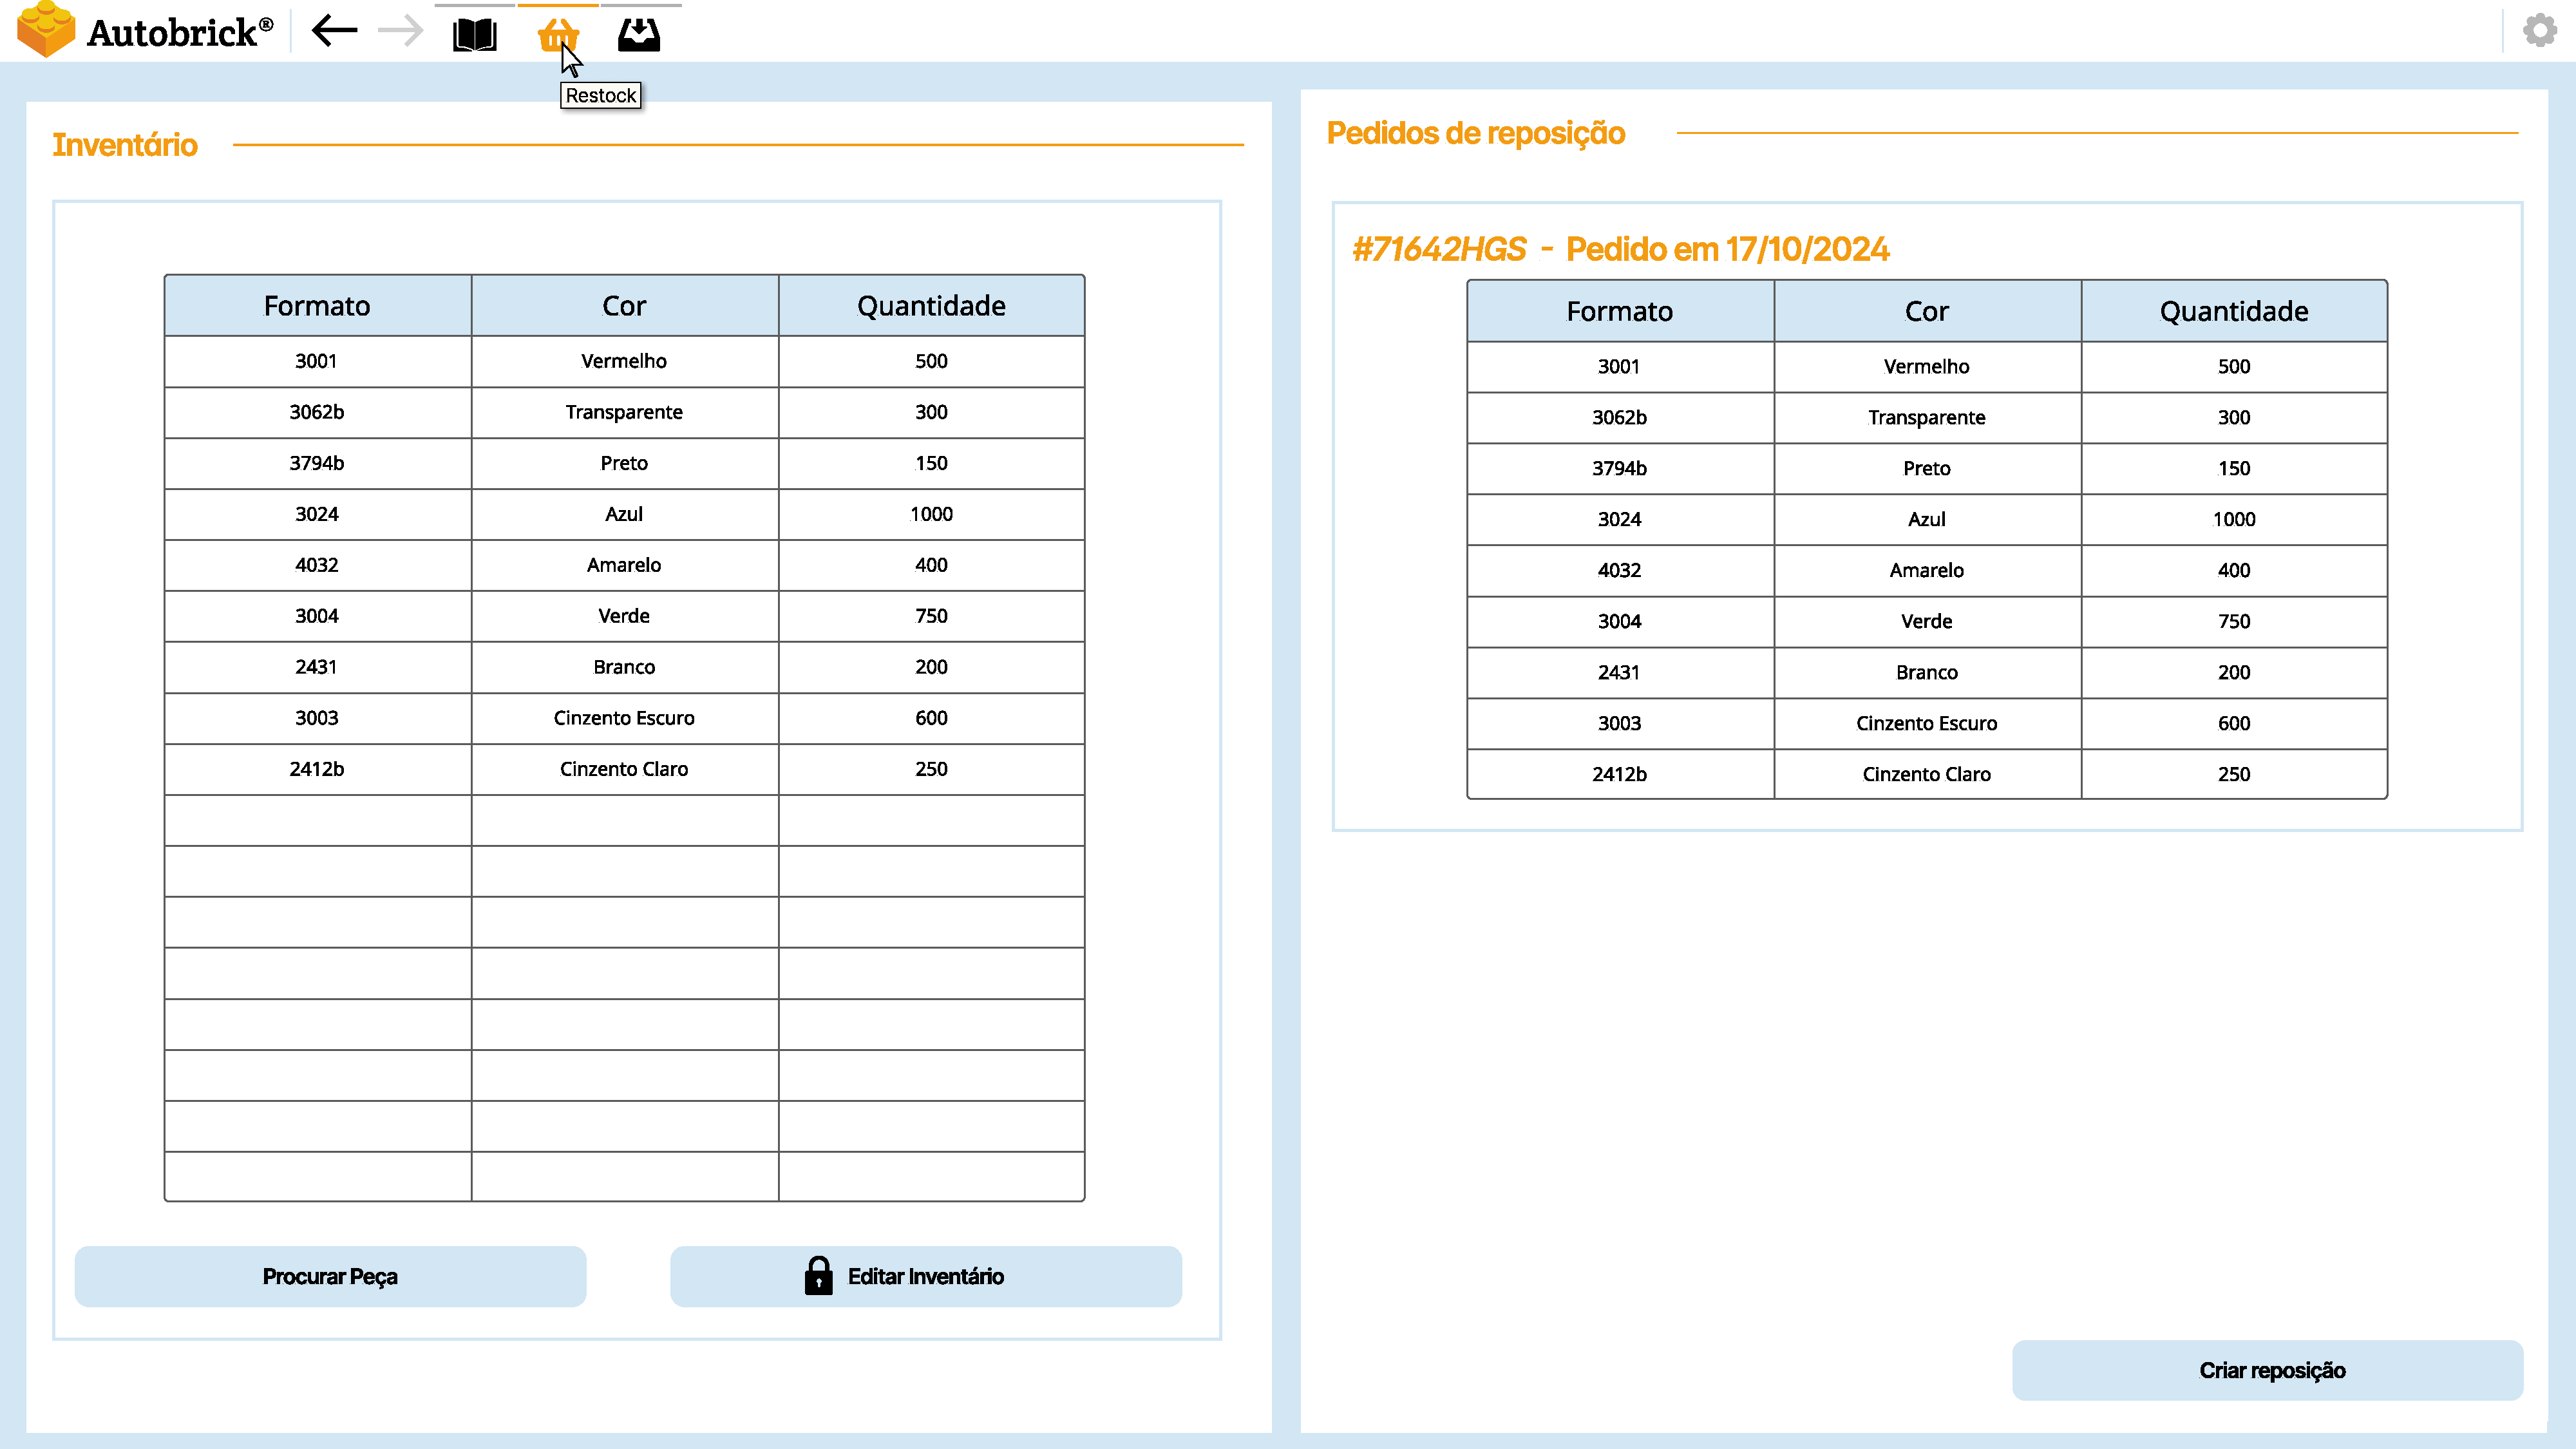
\includegraphics[width=0.99\linewidth, frame]{images/Restock I.pdf}
            \caption{Página de inventário}
            \label{fig:Inventário}
        \end{figure}
    
        Nesta página é possivel consultar o inventário de peças disponíveis (ver 2.4.1). Ainda nesta página é dada opção de fazer uma reposição manual (Figura~\ref{fig:Reposição})(ver use case 3.3.2.1) e é dada a possibilidade de editar a quantidade disponível de uma dada peça, caso esta opção seja selecionada o utilizador deve inserir a palavra passe de administrador (Figura~\ref{fig:EditarInv1}) e inserir os dados da peça alterar (Figura~\ref{fig:EditarInv2}) 
    
        \begin{figure}[h!]
            \centering
            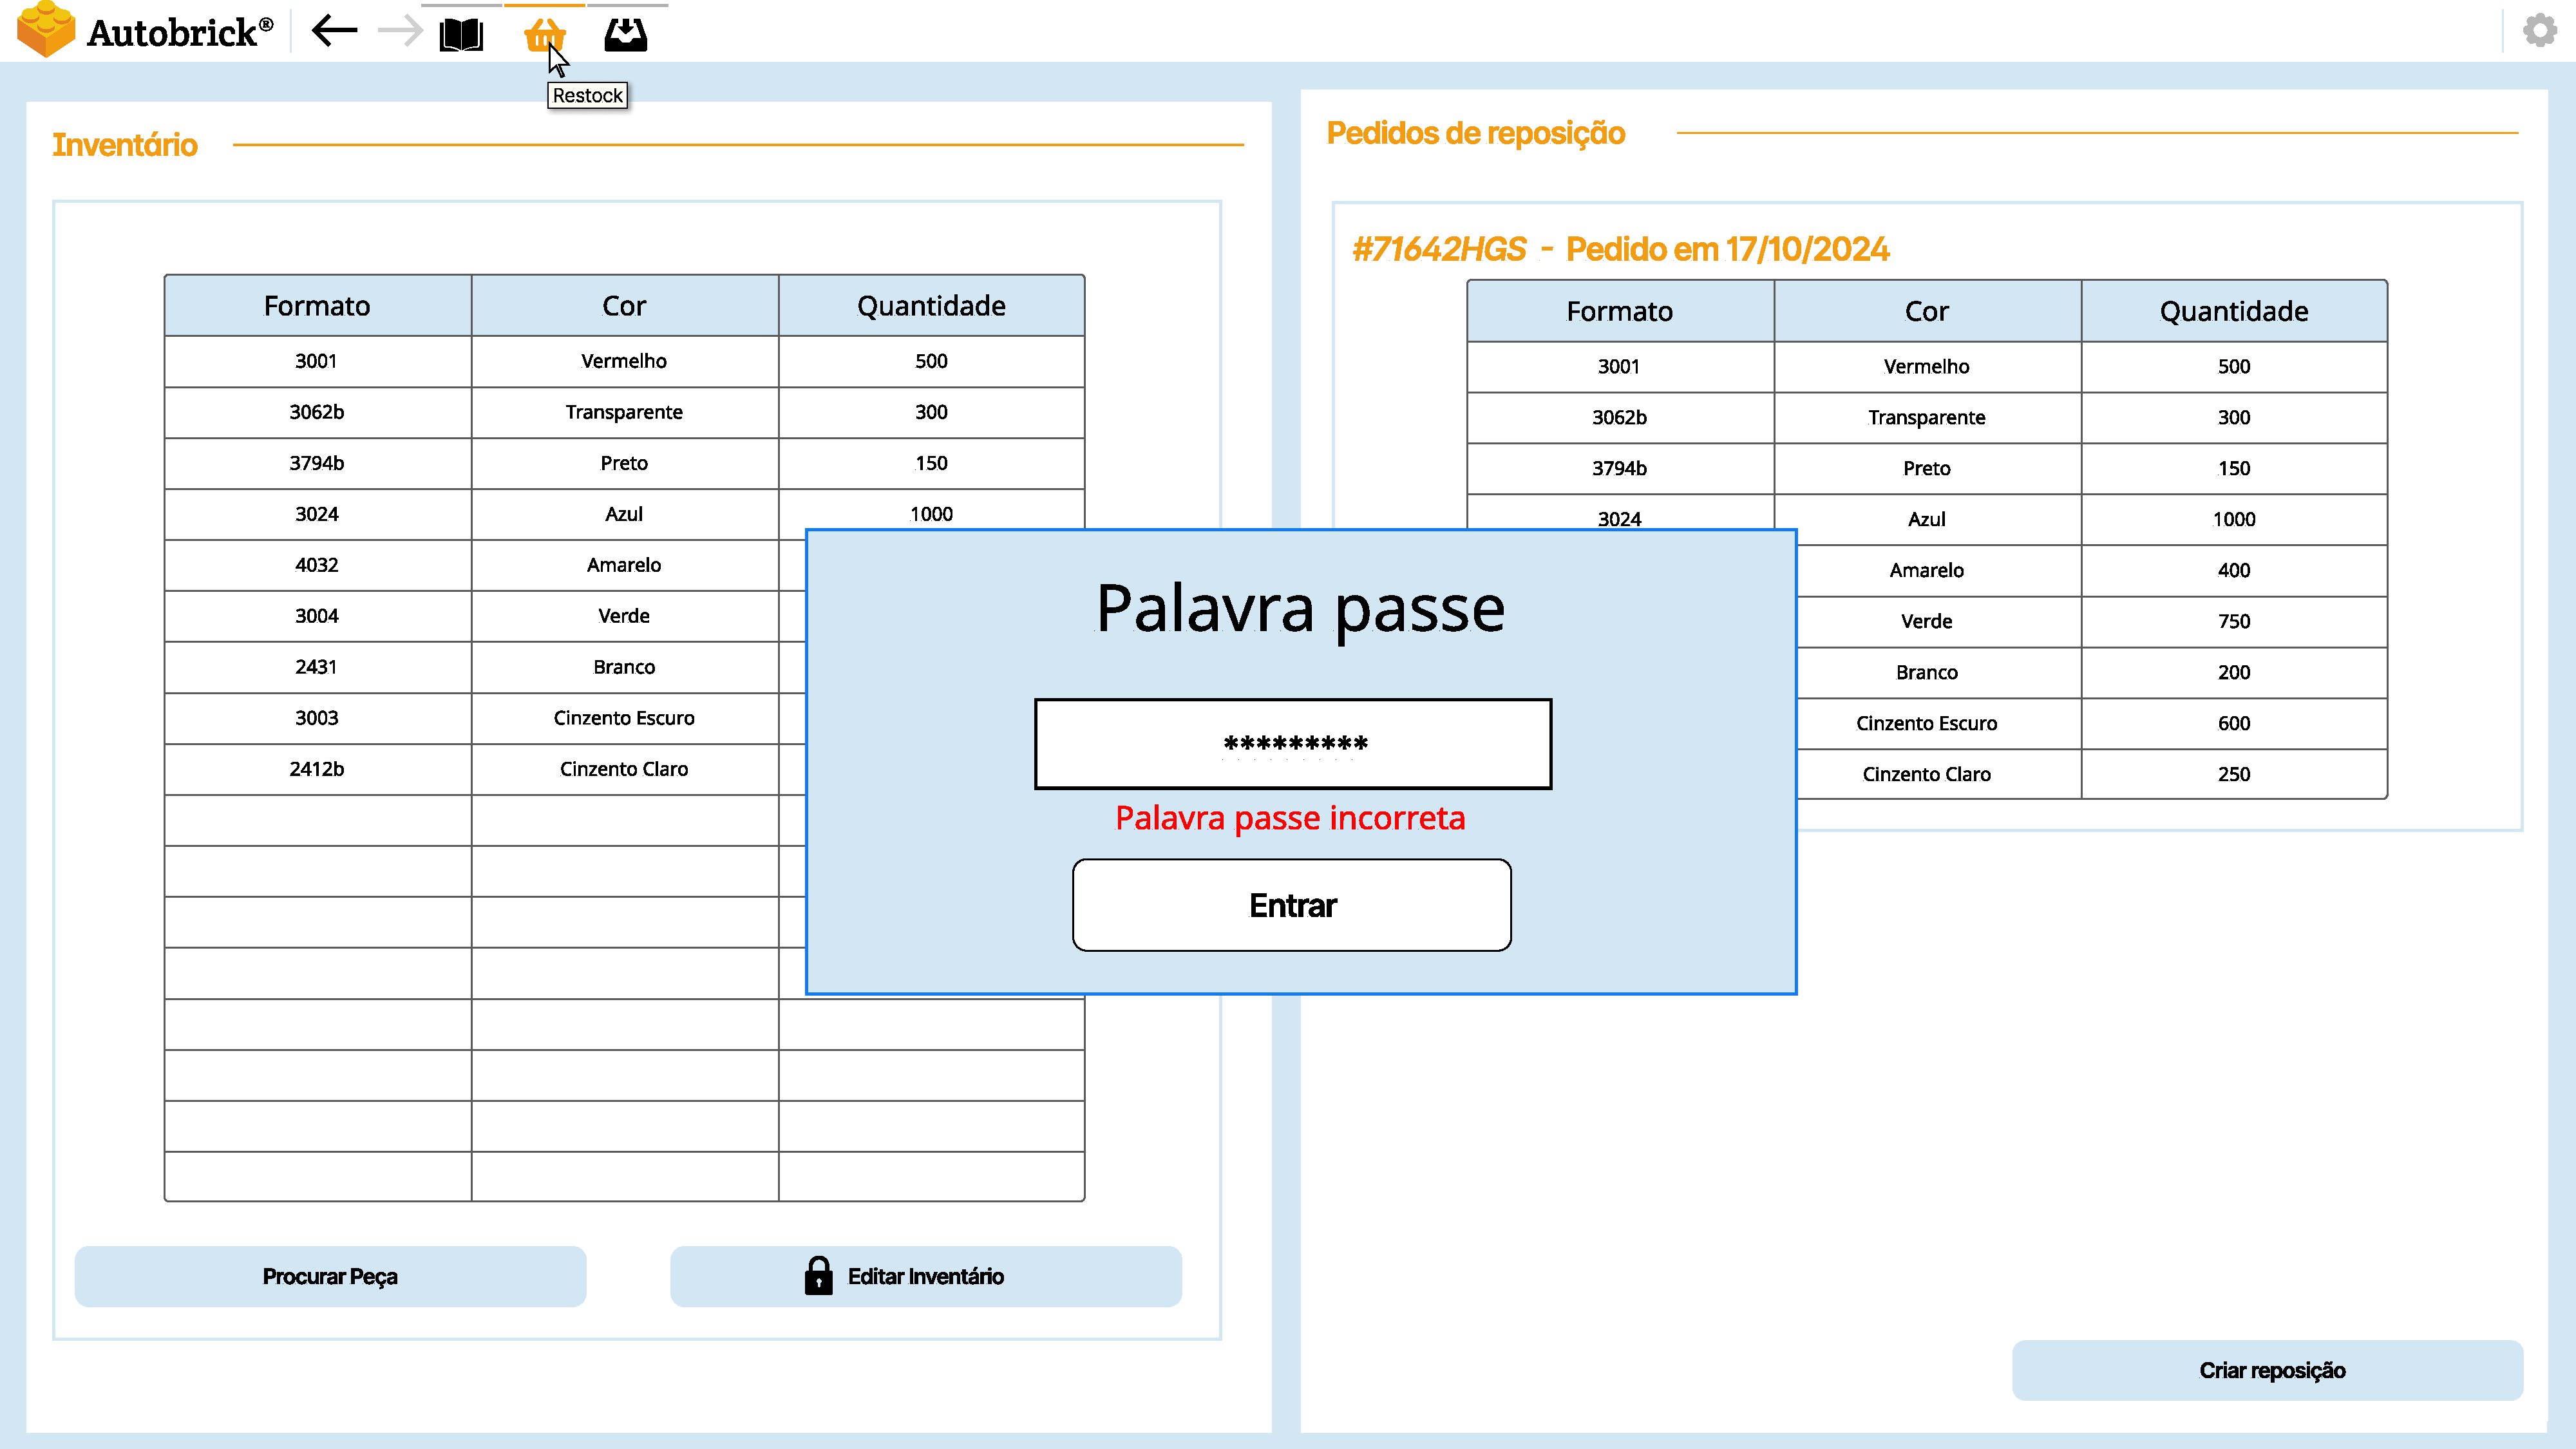
\includegraphics[width=0.99\linewidth, frame]{images/Admin Menu Alteração.pdf}
            \caption{Página de inventário após interação com botão de editar inventário (Palavra passe de administrador errada)}
            \label{fig:EditarInv1}
        \end{figure}
    
        \begin{figure}[h!]
            \centering
            \includegraphics[width=0.99\linewidth, frame]{images/Alterar inventário.pdf}
            \caption{Página de inventário após interação com botão de editar inventário (Após a palavra passe de administrador ser inserida)}
            \label{fig:EditarInv2}
        \end{figure}

        \clearpage    
        \begin{figure}
            \centering
            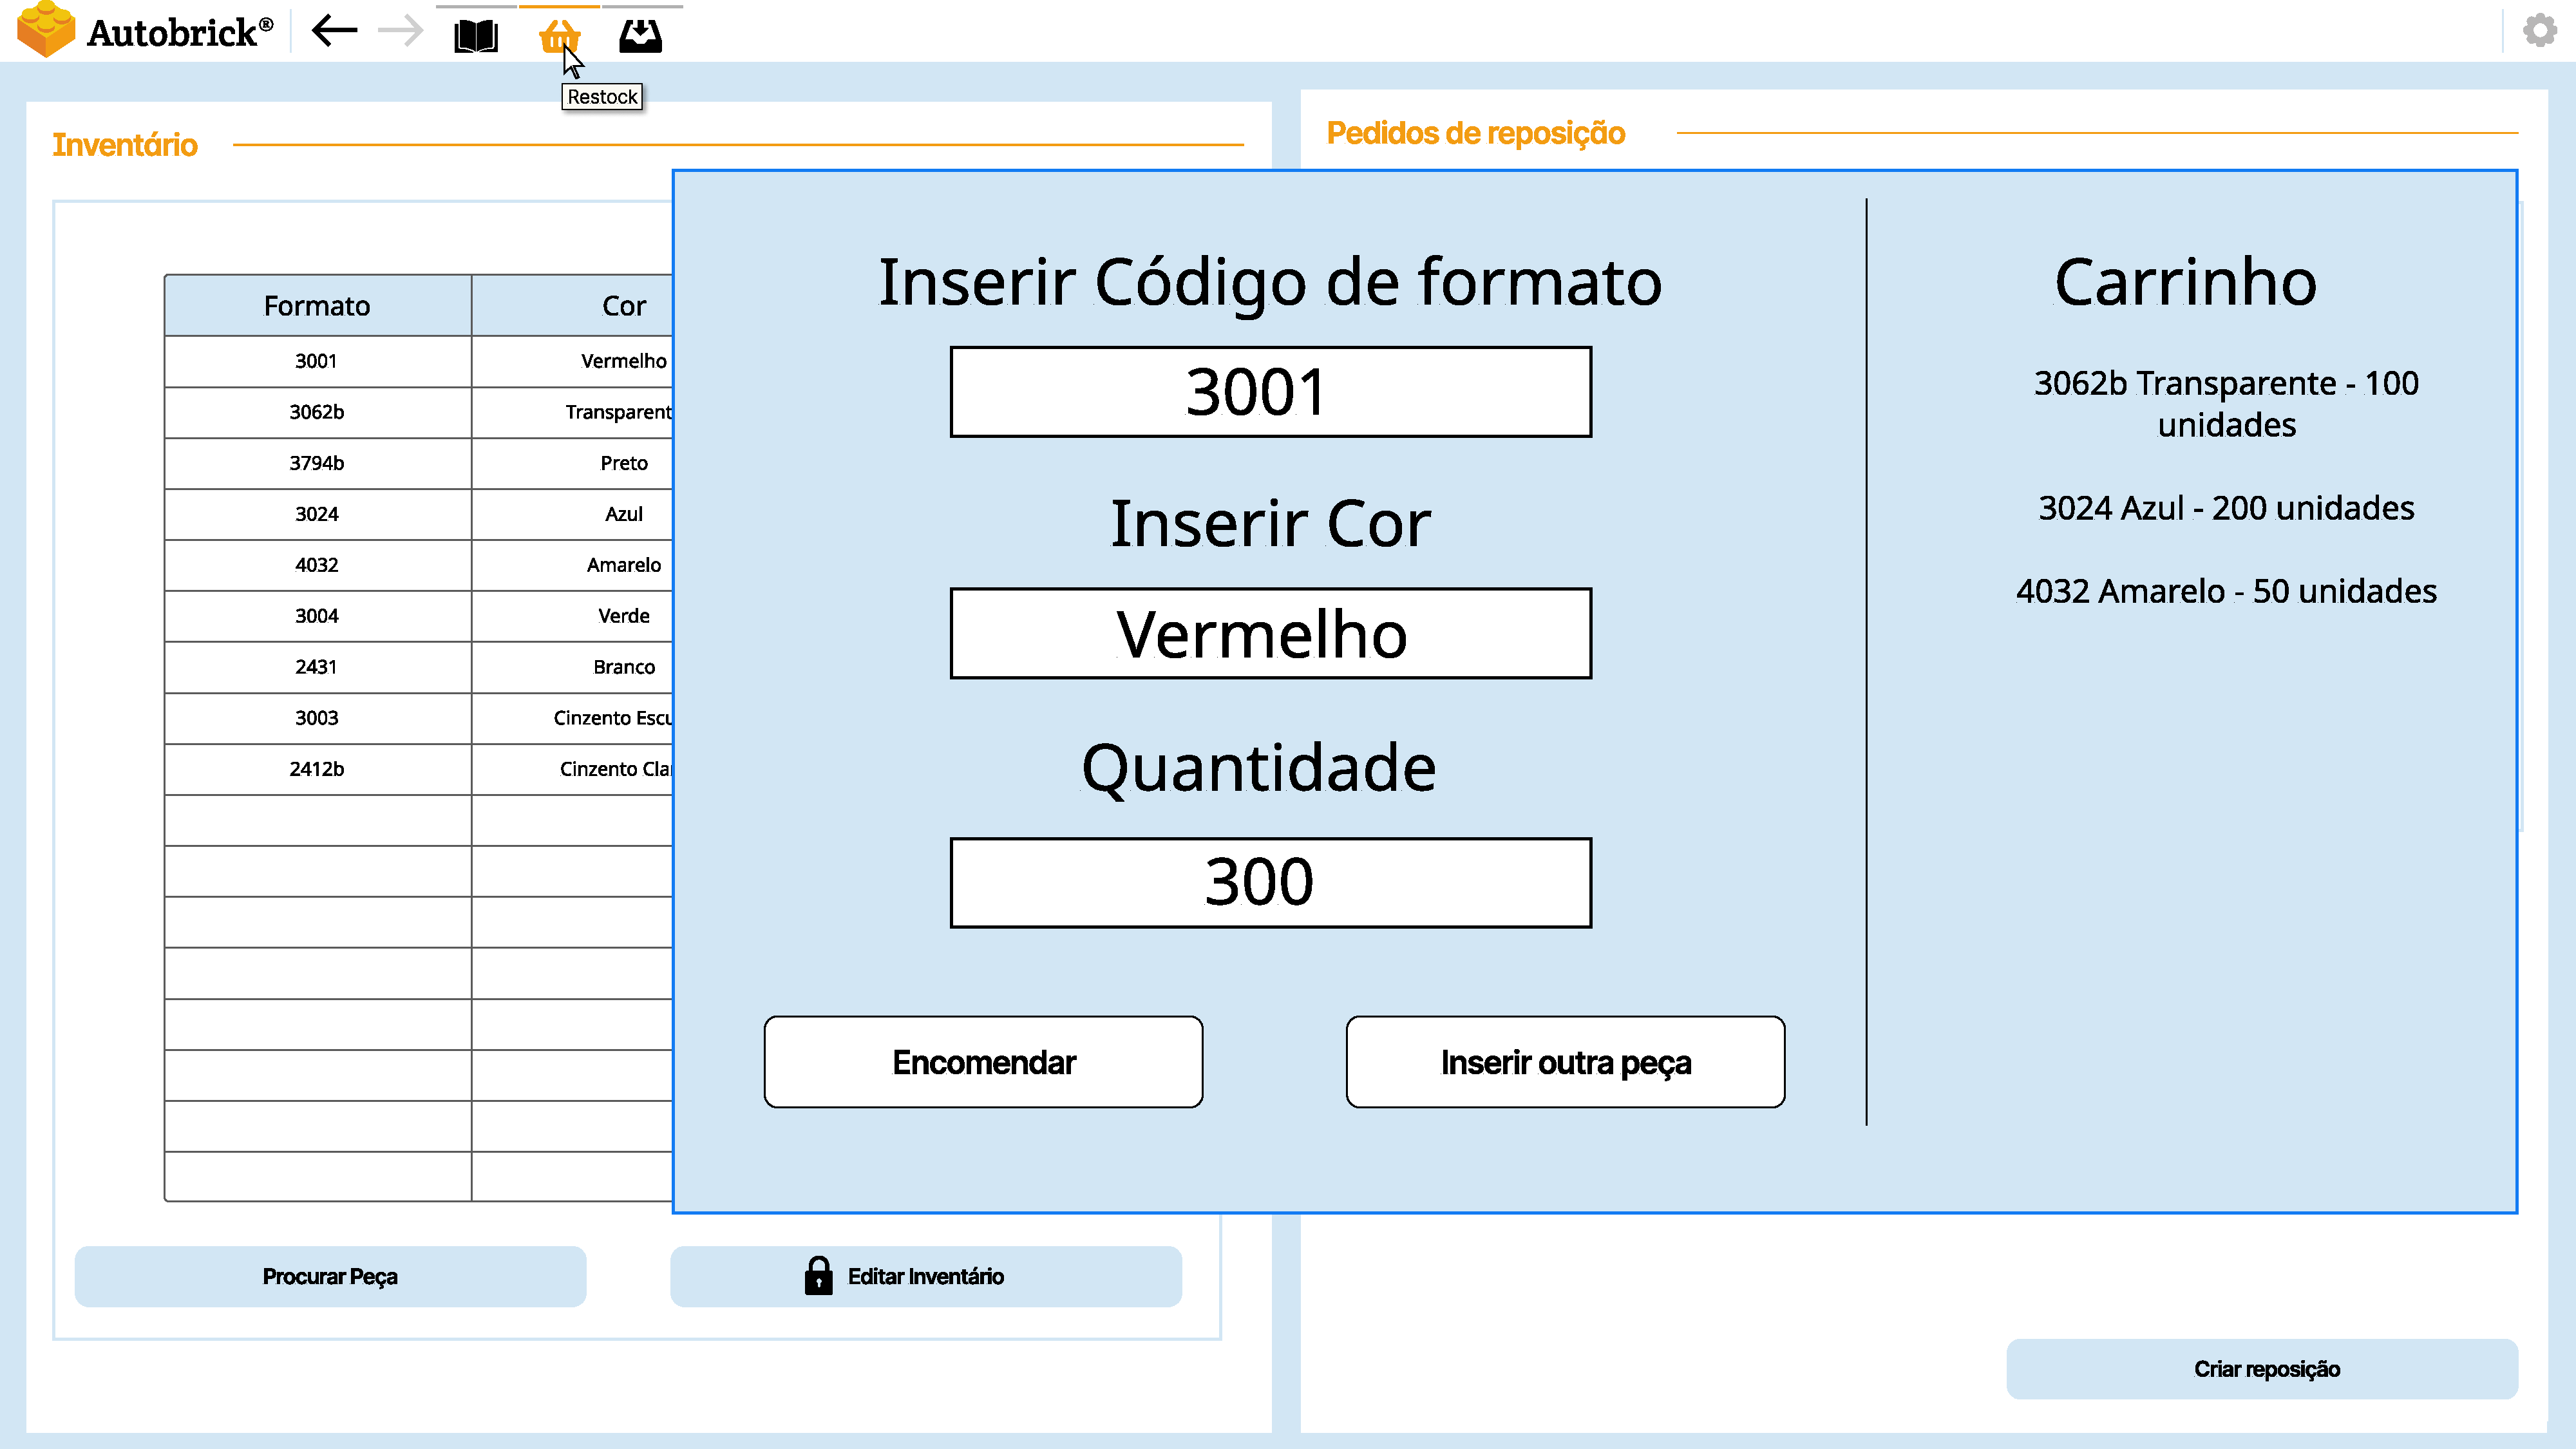
\includegraphics[width=0.99\linewidth, frame]{images/Restock Manual.pdf}
            \caption{Página de inventário após interação com botão de criar reposição}
            \label{fig:Reposição}
        \end{figure}

        \clearpage
        \subsection{Interfaces de Catálogo}
    
        \begin{figure}[ht]
            \centering
            \includegraphics[width=0.99\linewidth, frame]{images/Catálogo.pdf}
            \caption{Página de catálogo}
            \label{fig:Catálogo}
        \end{figure}

    Nesta páina é possível consultar uma lista com todos os modelos disponíveis (ver 3.3.3.1) bem como visualizar o manual de um modelo utilizando o botão "Visualizar Montagem" (ver 3.3.3.2).
    As figuras \ref{fig:Modelo Meio} e \ref{fig:Modelo Fim} mostram a página de instruções de um modelo de exemplo.
    
        \begin{figure}[h!]
            \centering
            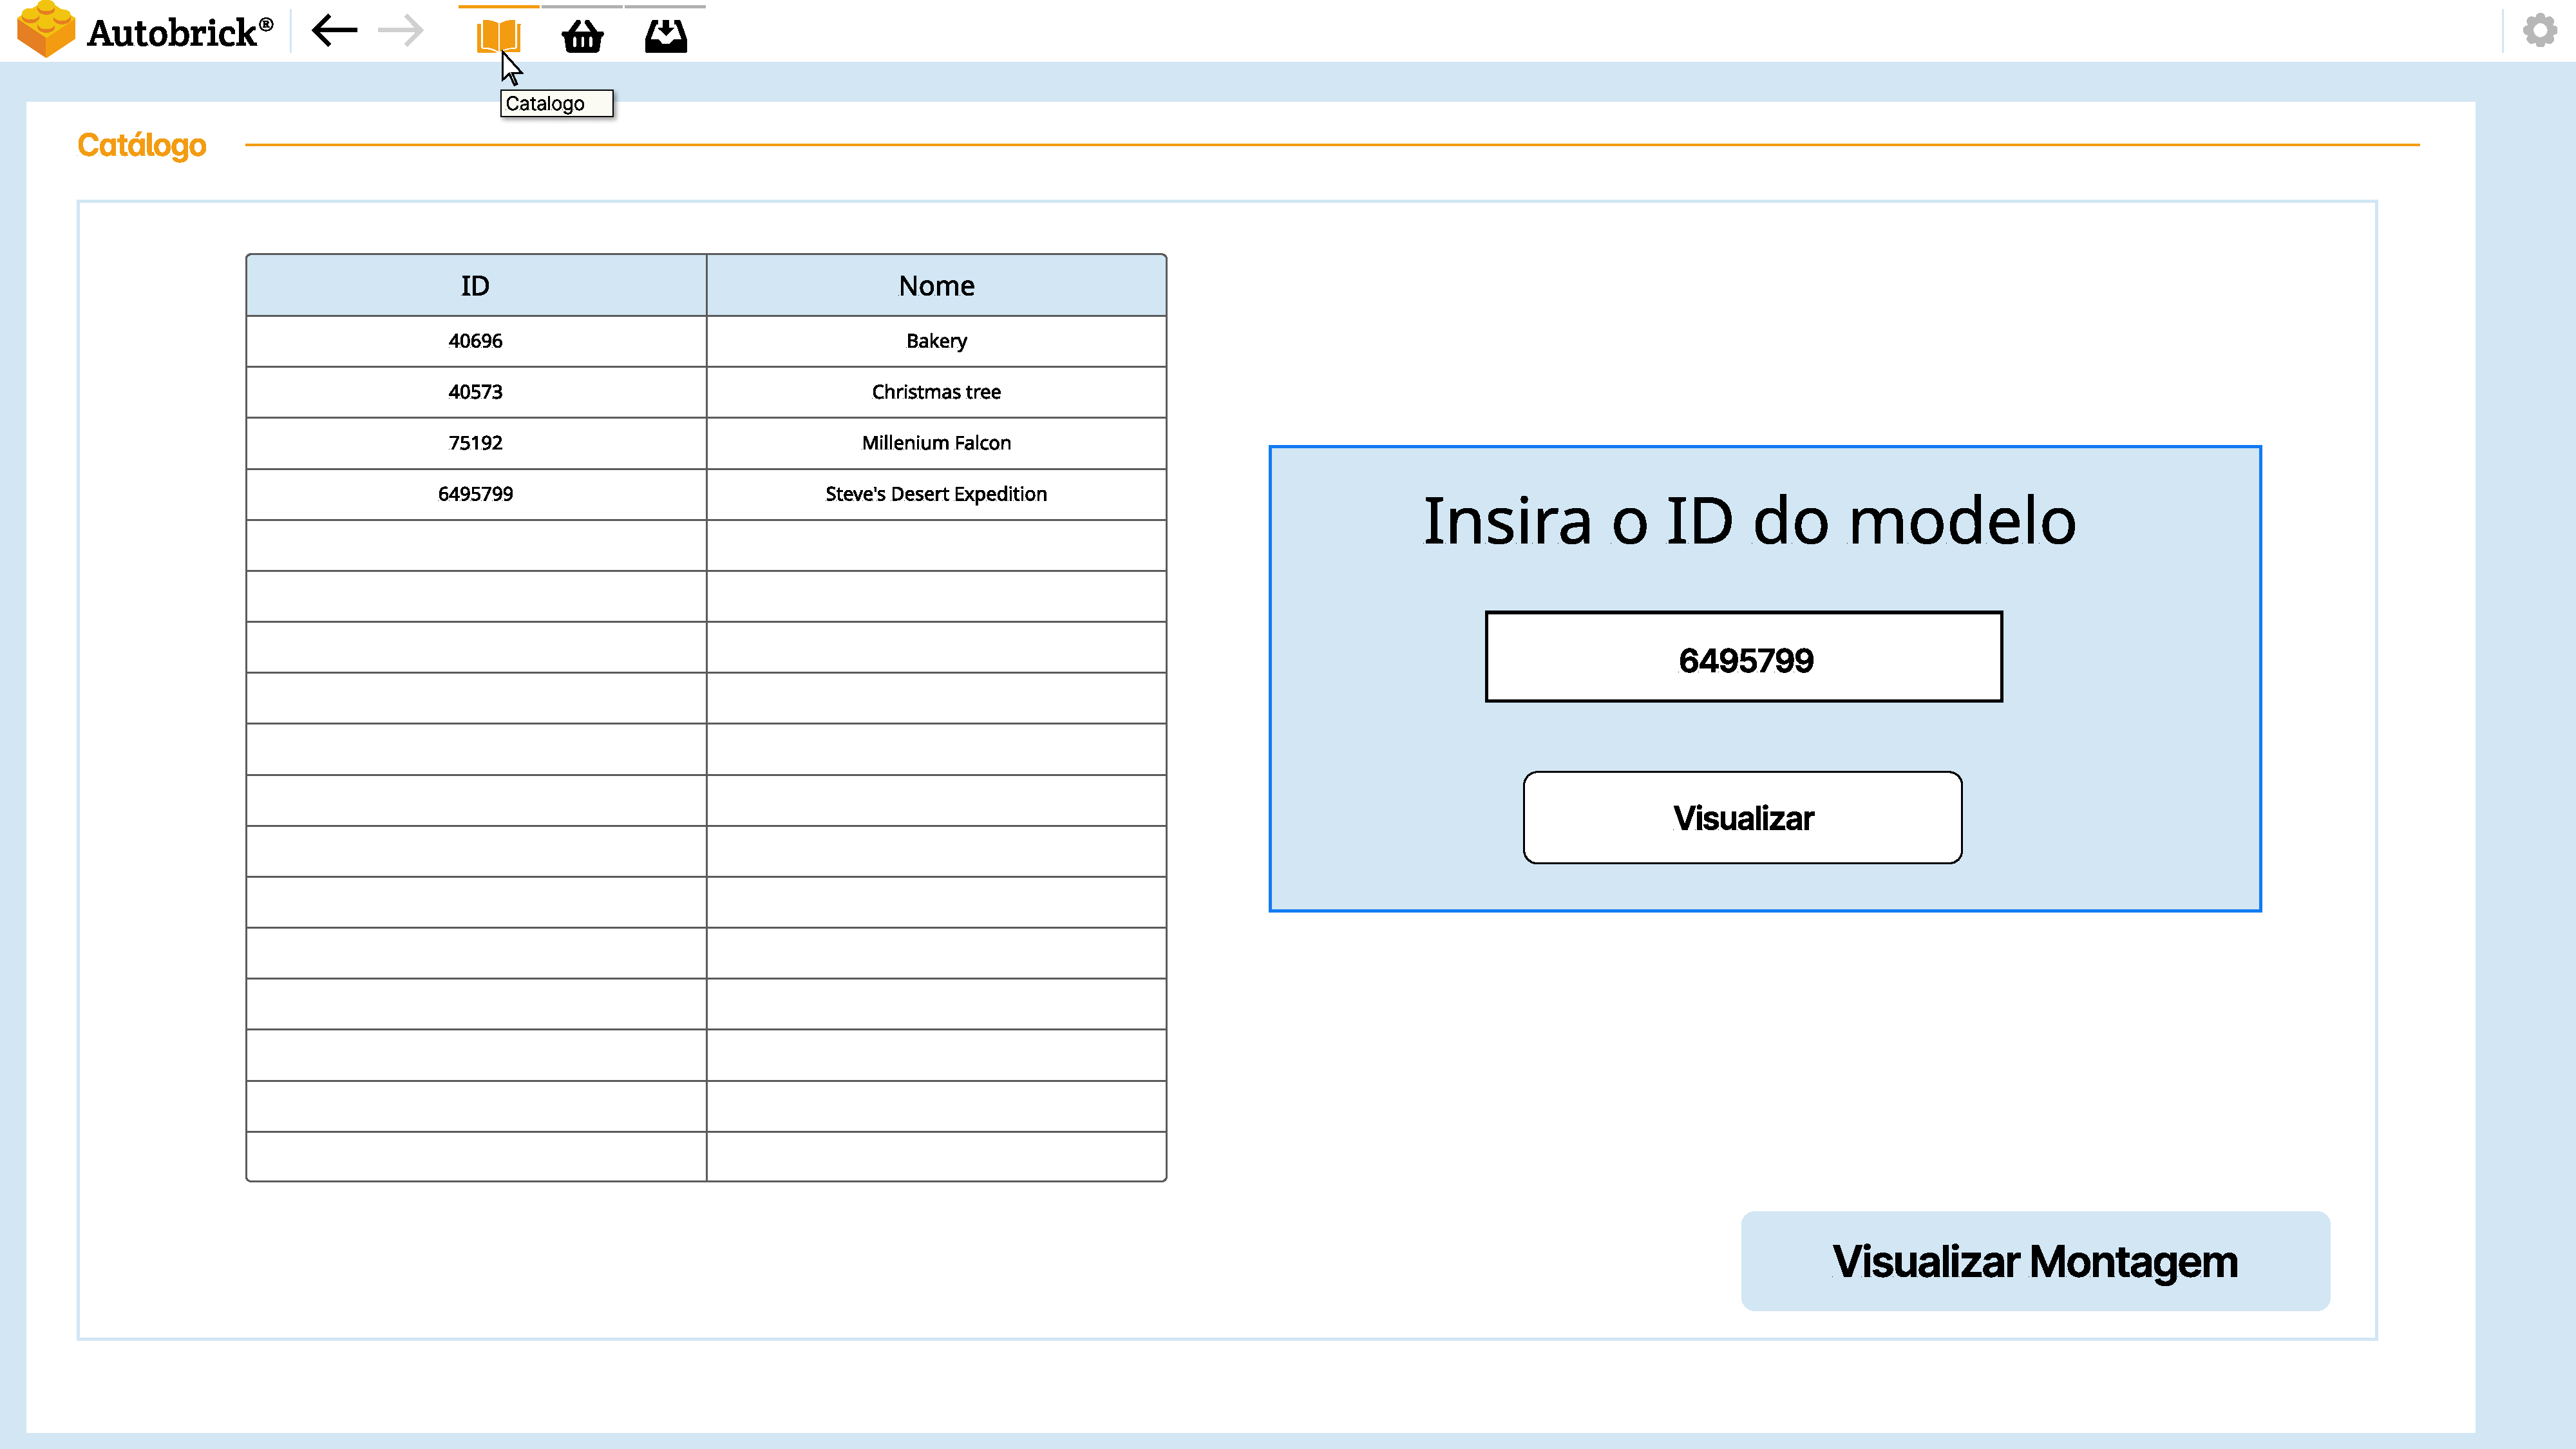
\includegraphics[width=0.99\linewidth, frame]{images/Visualizar montagem.pdf}
            \caption{Página de catálogo após interação com botão de visualizar montagem}
            \label{fig:Visualizar modelo}
        \end{figure}
    
        \begin{figure}[h!]
            \centering
            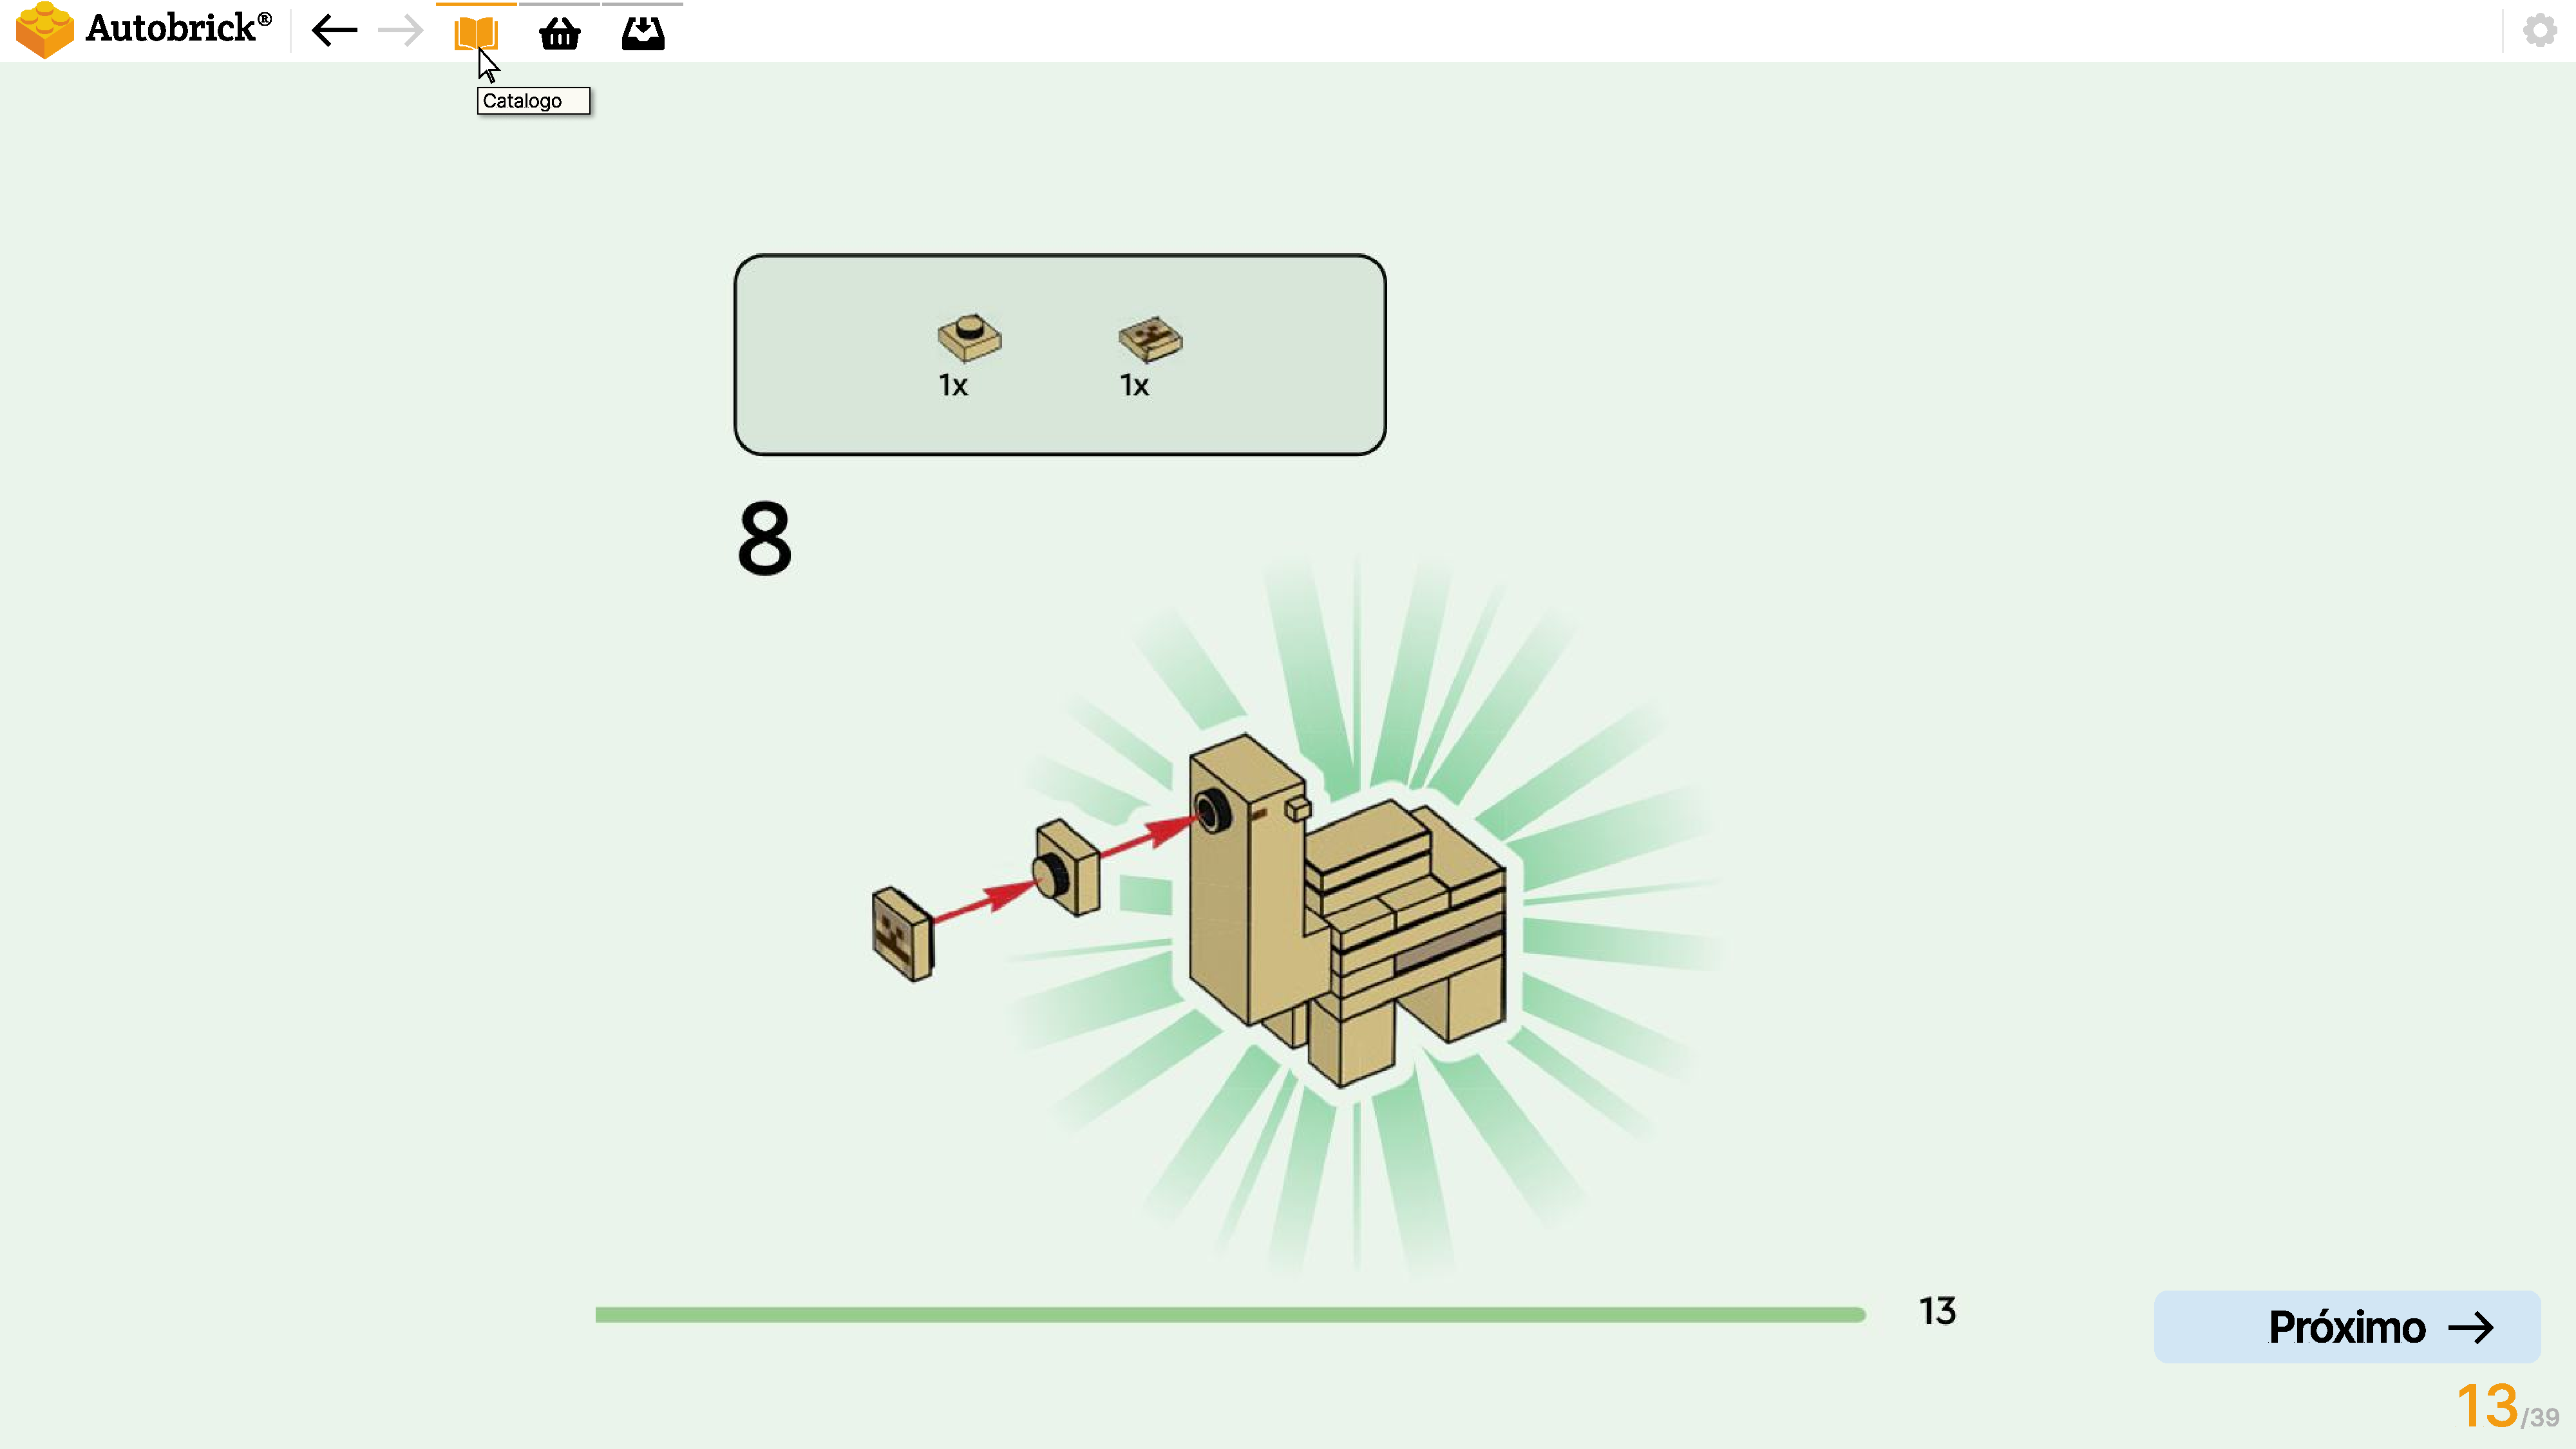
\includegraphics[width=0.99\linewidth, frame]{images/Instructions Manual I.pdf}
            \caption{Página de instruções para modelo (meio da montagem)}
            \label{fig:Modelo Meio}
        \end{figure}
    
        \begin{figure}[h!]
            \centering
            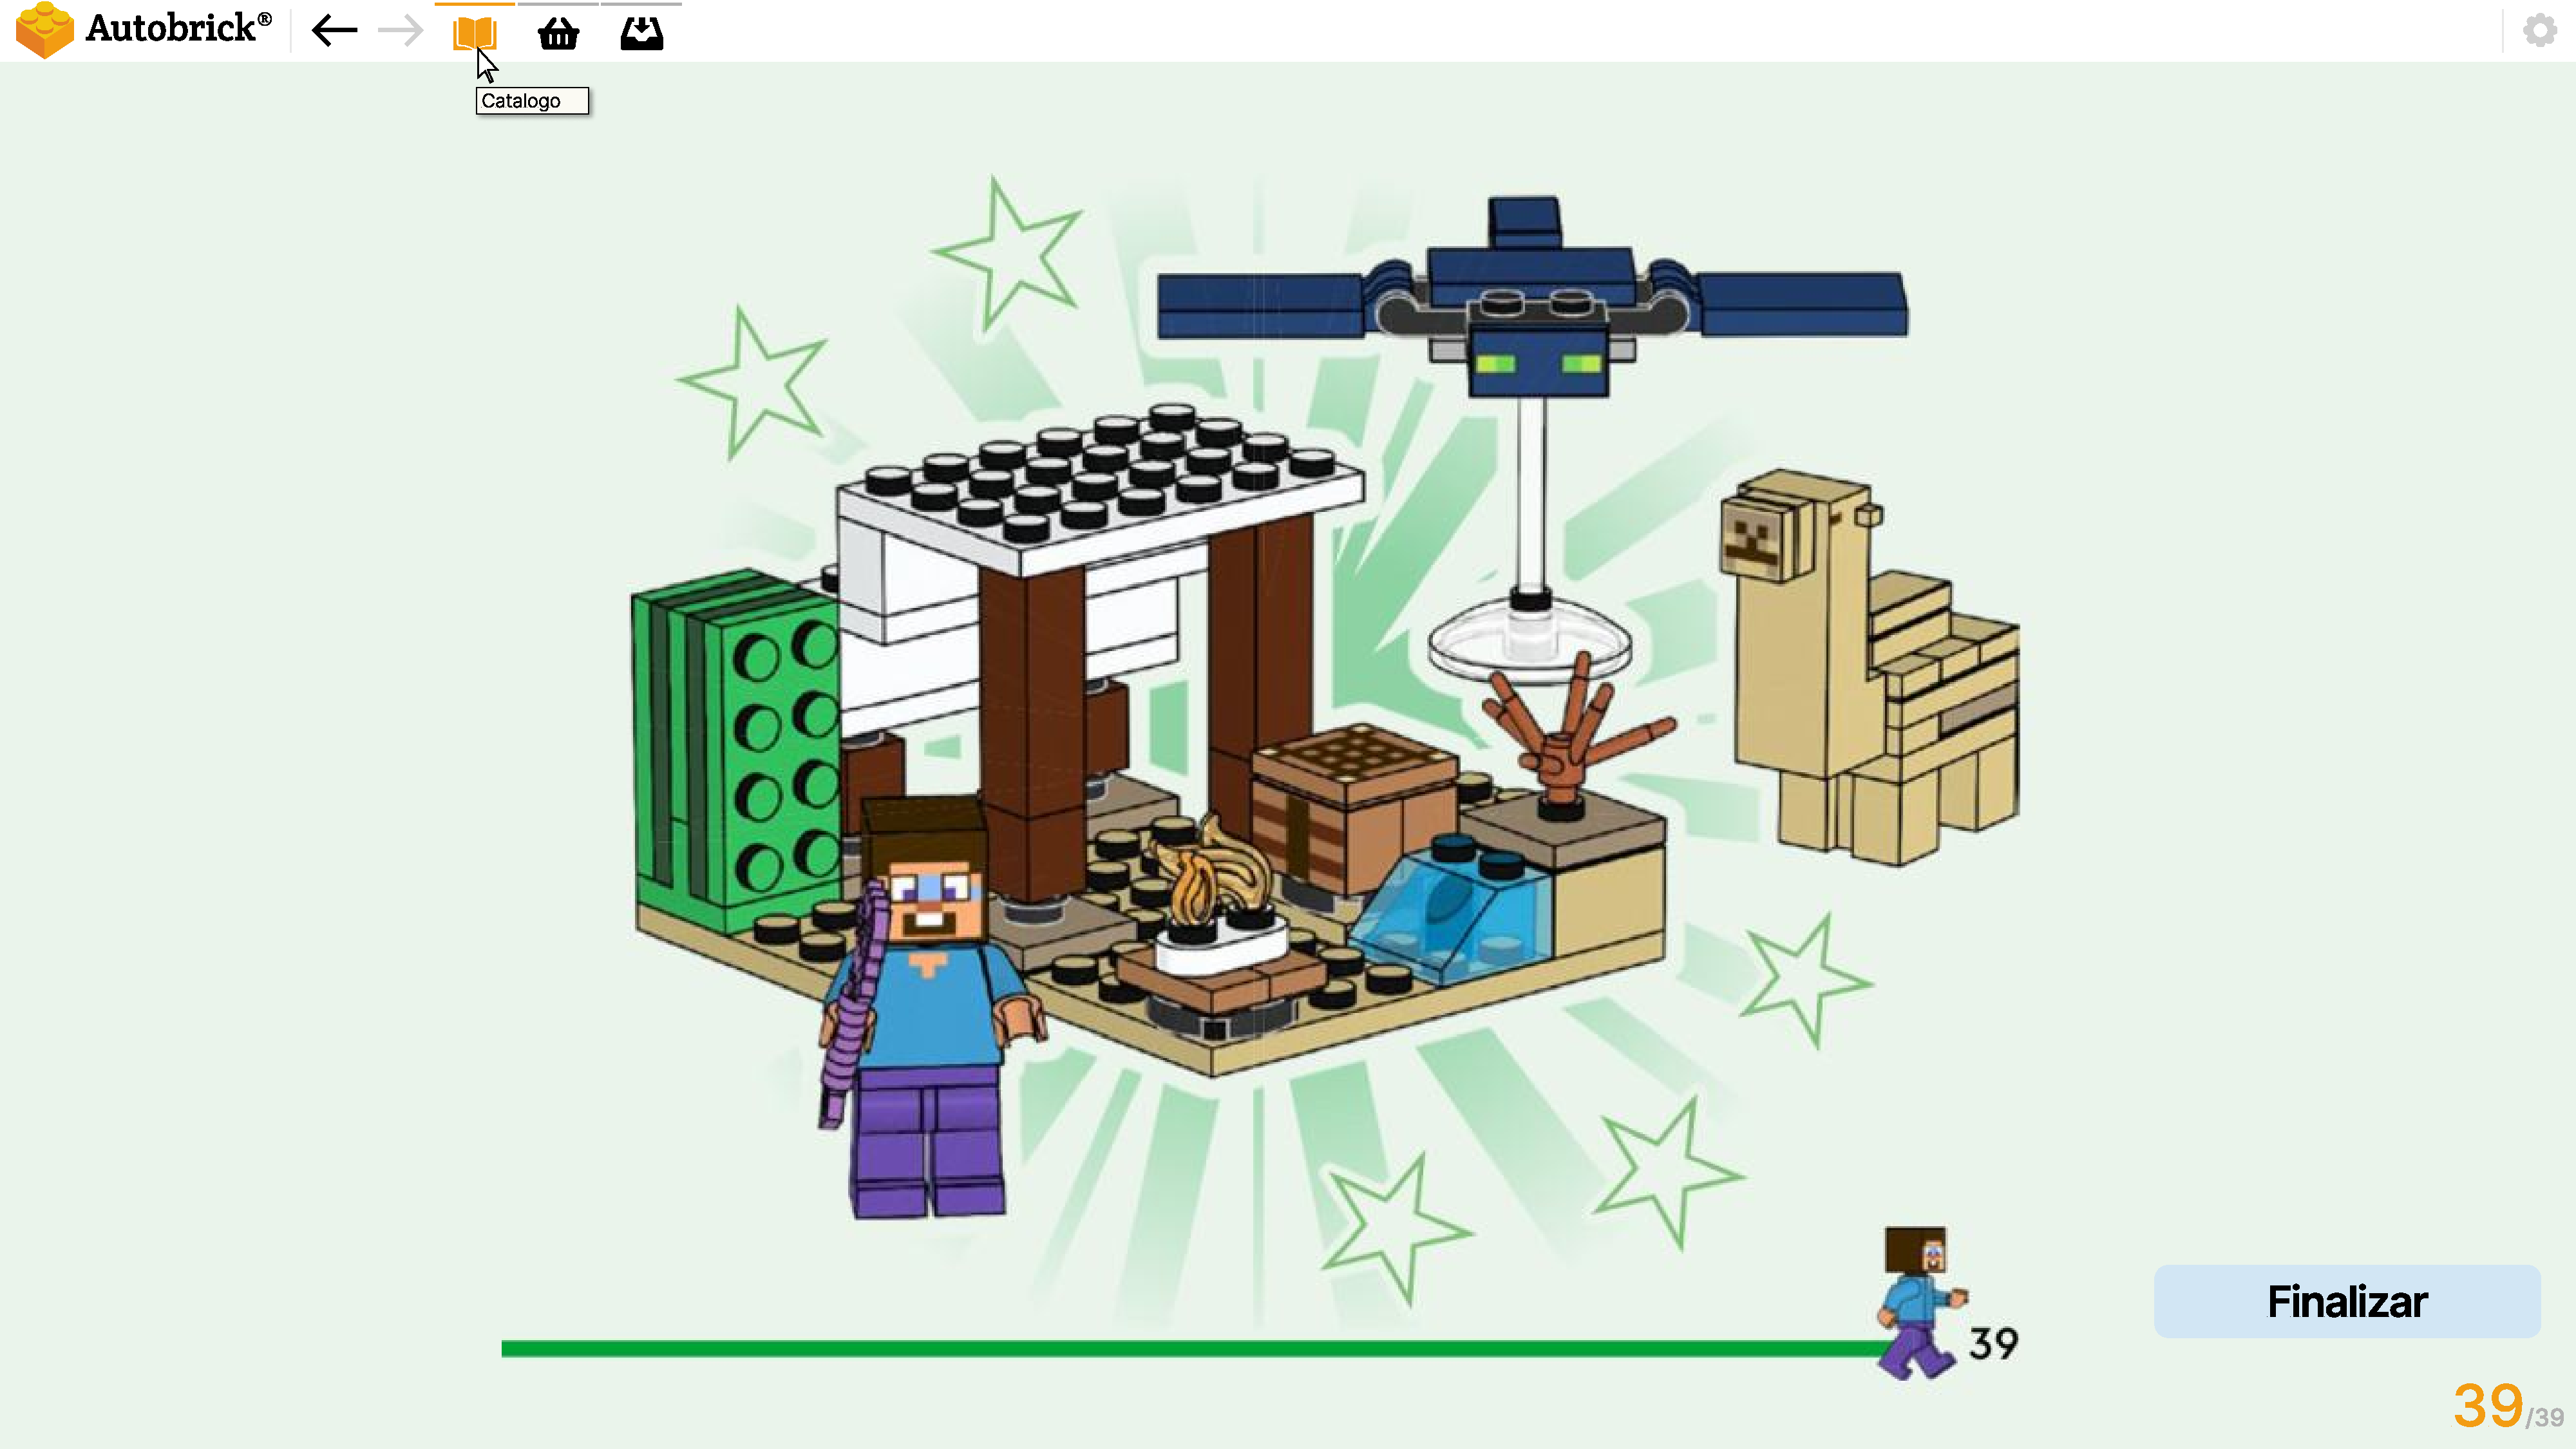
\includegraphics[width=0.99\linewidth, frame]{images/Instructions Manual II.pdf}
            \caption{Página de instruções para modelo (fim da montagem)}
            \label{fig:Modelo Fim}
        \end{figure}
    
%==========================================================================
% END #5 - ESBOÇO DOS INTERFACES DO SISTEMA
%==========================================================================
%==========================================================================
% BEGIN #6 - IMPLEMENTAÇÃO
% Descrição detalhada do processo de implementação realizado, referindo as opções de desenvolvimento que foram adotadas e as decisões tomadas. Apresentação da estrutura da aplicação desenvolvida e de cada um dos seus serviços, ilustrando um ou dois processos que tenham sido implementados. Reportar o desempenho da aplicação e, em particular, de cada um dos serviços implementados. 

% 1) Apresentação e descrição do processo de implementação realizado.

% 2) Apresentação da aplicação e explicação dos serviços implementados.

% 3) Analise e avaliação da aplicação desenvolvida.

%==========================================================================


\chapter{Implementação da Aplicação}
    
    \section{Descrição do Processo de Implementação}

            O arranque da fase de implementação inaugurou-se com um debate sobre qual \textit{framework} de desenvolvimento enquadrada no \textit{ASP.NET} se via mais adequado tanto para o contexto em mão e para a equipa. Dada a preferência por linguagens já familiares, escolheu-se o \textit{Blazor} ao invés do mais ubíquo ASP.NET Core MVC, por permitir a escrita em \textit{C\#} para todas as camadas do programa.   
                
        \newpage
        \subsection{\textit{Back End}}

            \subsubsection{Tecnologias/Ferramentas Utilizadas}
                    Dado o contexto de .NET, foi decidido o recurso ao SQL Server como gestor de base de dados, por ser a opção mais comum e à responsabilidade da mesma Microsoft, o que induz maior compatibilidade, melhor apoio técnico e mais facilidade na potencial integração de recém-contratados para mantuenção do sistema no futuro. 
        
            \subsubsection{Acesso a Dados}
                % Estratégia de Acesso a Dados (Database-First/DAOs vs Code-First/Entity Framework)
                    A estratégia de acesso a dados foi alvo de ponderação sobre o uso de \textit{Entity Framework Core (EFCore)}, que implica a estipulação \textit{a priori} de modelos lógicos suportados por parâmetros que permitem a inferência automática dunm contexto de base de dados, controladores e de páginas genéricas para ponto de partida da camada de apresentação. Este paradigma denomina-se "código primeiro". No entanto, o facto de já haver tabelas definidas em antemão fez com que se utilizasse antes o método "base de dados primeiro", com modelos feitos manualmente. Os modelos são então instanciados via objetos de acesso a dados (DAOs), que abstraem as interações necessárias com a base de dados.

                % Queries de Criação das Tabelas
                    Foi elaborado o \textit{script} visto à frente para a criação da base de dados do sistema.
                    \newpage
                    \lstinputlisting[breaklines,basicstyle=\ttfamily\tiny,label=lst:sqlcreatedb]{code/sqlcreatedb.sql}
                % Definição de Objetos de Acesso a Dados (DAOs)
                    O programa acede à base de dados graças à biblioteca de classes \texttt{DataAccess} adicionada como dependência, que define \texttt{[Order|Piece|Set|User]DAO} como DAOs. São parecidos no sentido em que todos disponibilizam métodos para interação com a base de dados, mas diferem em termos da temática para qual se orientam. Deste modo, há um maior grau de separação de matérias no código, tornando-o mais organizado. Ao ser do interesse a certo método na camada de negócio interagir com a base de dados por um motivo primariamente referente a encomendas, deve partir de \texttt{OrderDAO}. Esta fragmentação é cada vez mais útil à medida que o sistema cresce em complexidade de modelos e subsistemas.
                
                    Estes DAOs comunicam com a base de dados graças à classe \texttt{DatabaseAccess}, que fornece a \textit{string} de conexão.
            \newpage
            \subsubsection{Lógica de Negócio}
            
                % Definição de Modelos de Dados (Com base no domínio estabelecido no capítulo 3) 
                    Foram definidos os modelos de dados na biblioteca de classes \texttt{Models} adicionada como dependência, servindo a função não só de entidades representantes dos dados mas também de modelos de apresentação (\textit{view models}). É de frisar que, no contexto duma aplicação de maior escala, seria preferível o estabelecimento de modelos de apresentação completamente separados dos modelos de dados, pois é uma prática promotora da assincronicidade de desenvolvimento que permite aos encarregados pela camada apresentativa não depender de potenciais alterações feitas por programadores mais abaixo na cadeia.
                    \lstinputlisting[breaklines,basicstyle=\ttfamily\tiny,label=lst:models]{code/Models.cs}
                    % Piece, Set, Order, User    
                
                % Lógica em Páginas Razor
                    \newpage
                    As páginas \textit{Razor} possibilitaram a implementação de lógica de negócio em conjunto com o formato HTML das páginas. Isto resultou num certo acoplamento de código que, num caso de maior escala, seria preferível de abstrair para subsistemas, assim conseguindo potencialmente fazer do \textit{back end} uma mera interface de programação (API) e flexivelmente substituir o \textit{front end} por completo se necessário.

                    Sendo um programa de gestão, a maioria dos requisitos assentam na visualização de dados. Tal torna a camada de lógica de negócio relativamente "fina" e, com isso em mente, tomou-se a decisão de fazer chamadas diretamente das páginas Razor aos DAOs. A título de exemplo, observe-se o excerto de código abaixo, incluído na página para pedido de reposição manual. O método \texttt{Submit} é chamado quando o botão de igual nome é carregado.
                    
                    \lstinputlisting[breaklines,basicstyle=\ttfamily\tiny, label=lst:restockrequest]{code/RestockRequest.cs}
                    
        \newpage
        \subsection{\textit{Front End}}

            \subsubsection{Tecnologias/Ferramentas Utilizadas}
                Graças ao uso de componentes Blazor e páginas Razor no geral, apenas foi necessária a utilização de HTML e CSS para dar à aplicação um estilo próprio e com um grau de fidelidade para com os esboços da interface elaborados na etapa anterior.
                
            \subsubsection{Mapa de Páginas}
                Observe-se um mapa de navegação pela aplicação. Nada é acessível ao utilizador antes de se autenticar, pelo que depois disso é-lhe apenas impedido o acesso à edição de inventário até à inserção duma senha administrativa válida.

                \begin{figure}[h!]
                    \centering
                    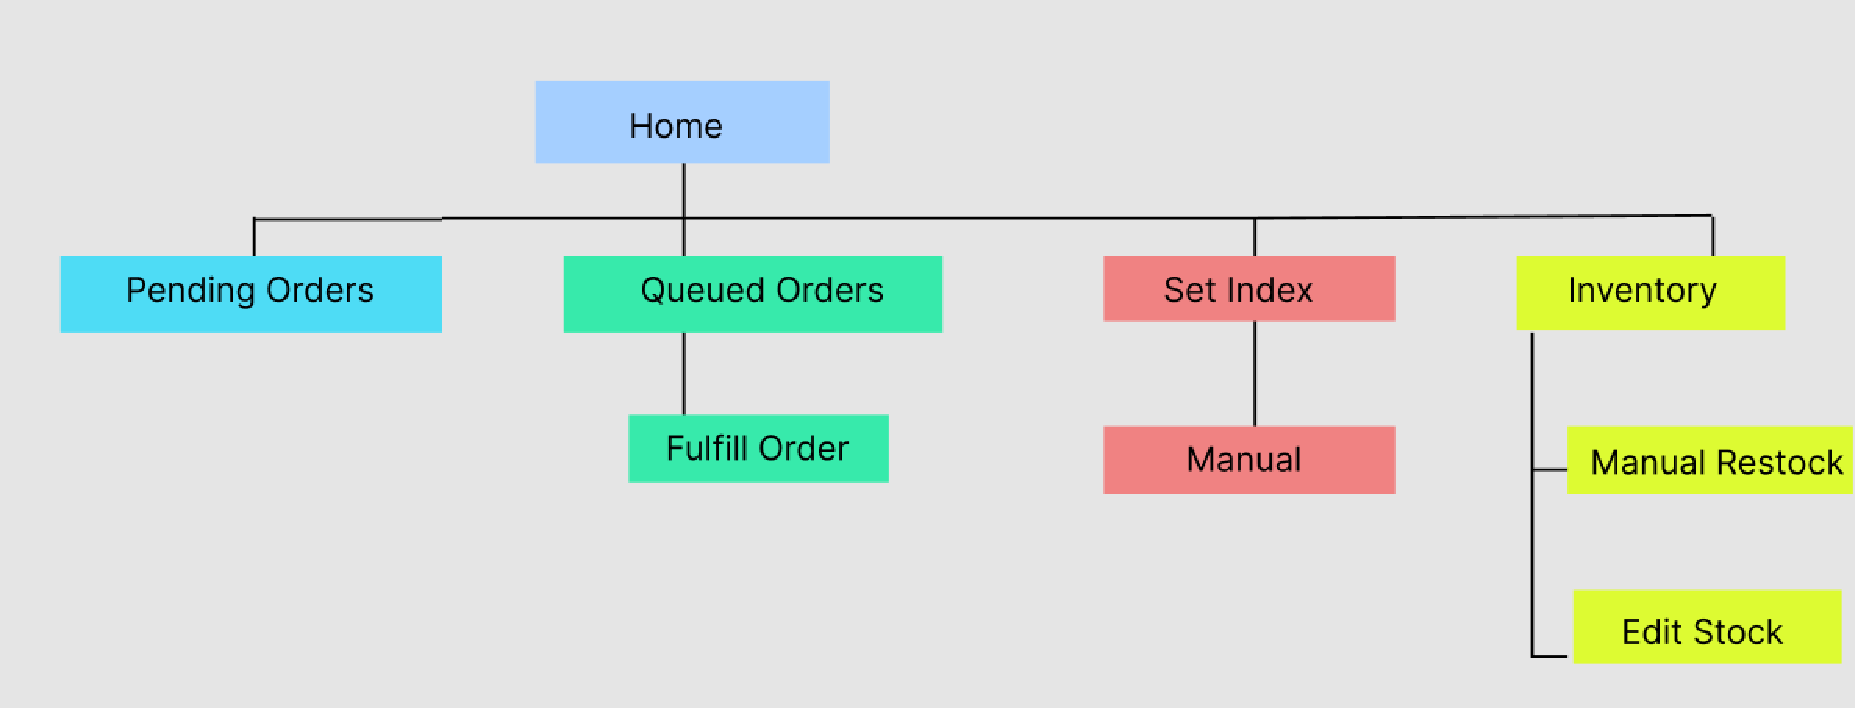
\includegraphics[width=0.99\linewidth, frame]{images/Site/sitemap.pdf}
                    \caption{Mapa de Páginas}
                    \label{fig:sitemap}
                \end{figure}
                
    \newpage
    \section{Serviços e Funcionamento} % Screenshots da app ficam nesta secção
        
            \subsection{Serviços Relativos a Utilizadores}
                \subsubsection{Sessões de Utilizador}

                            \begin{figure}[h!]
                                \centering
                                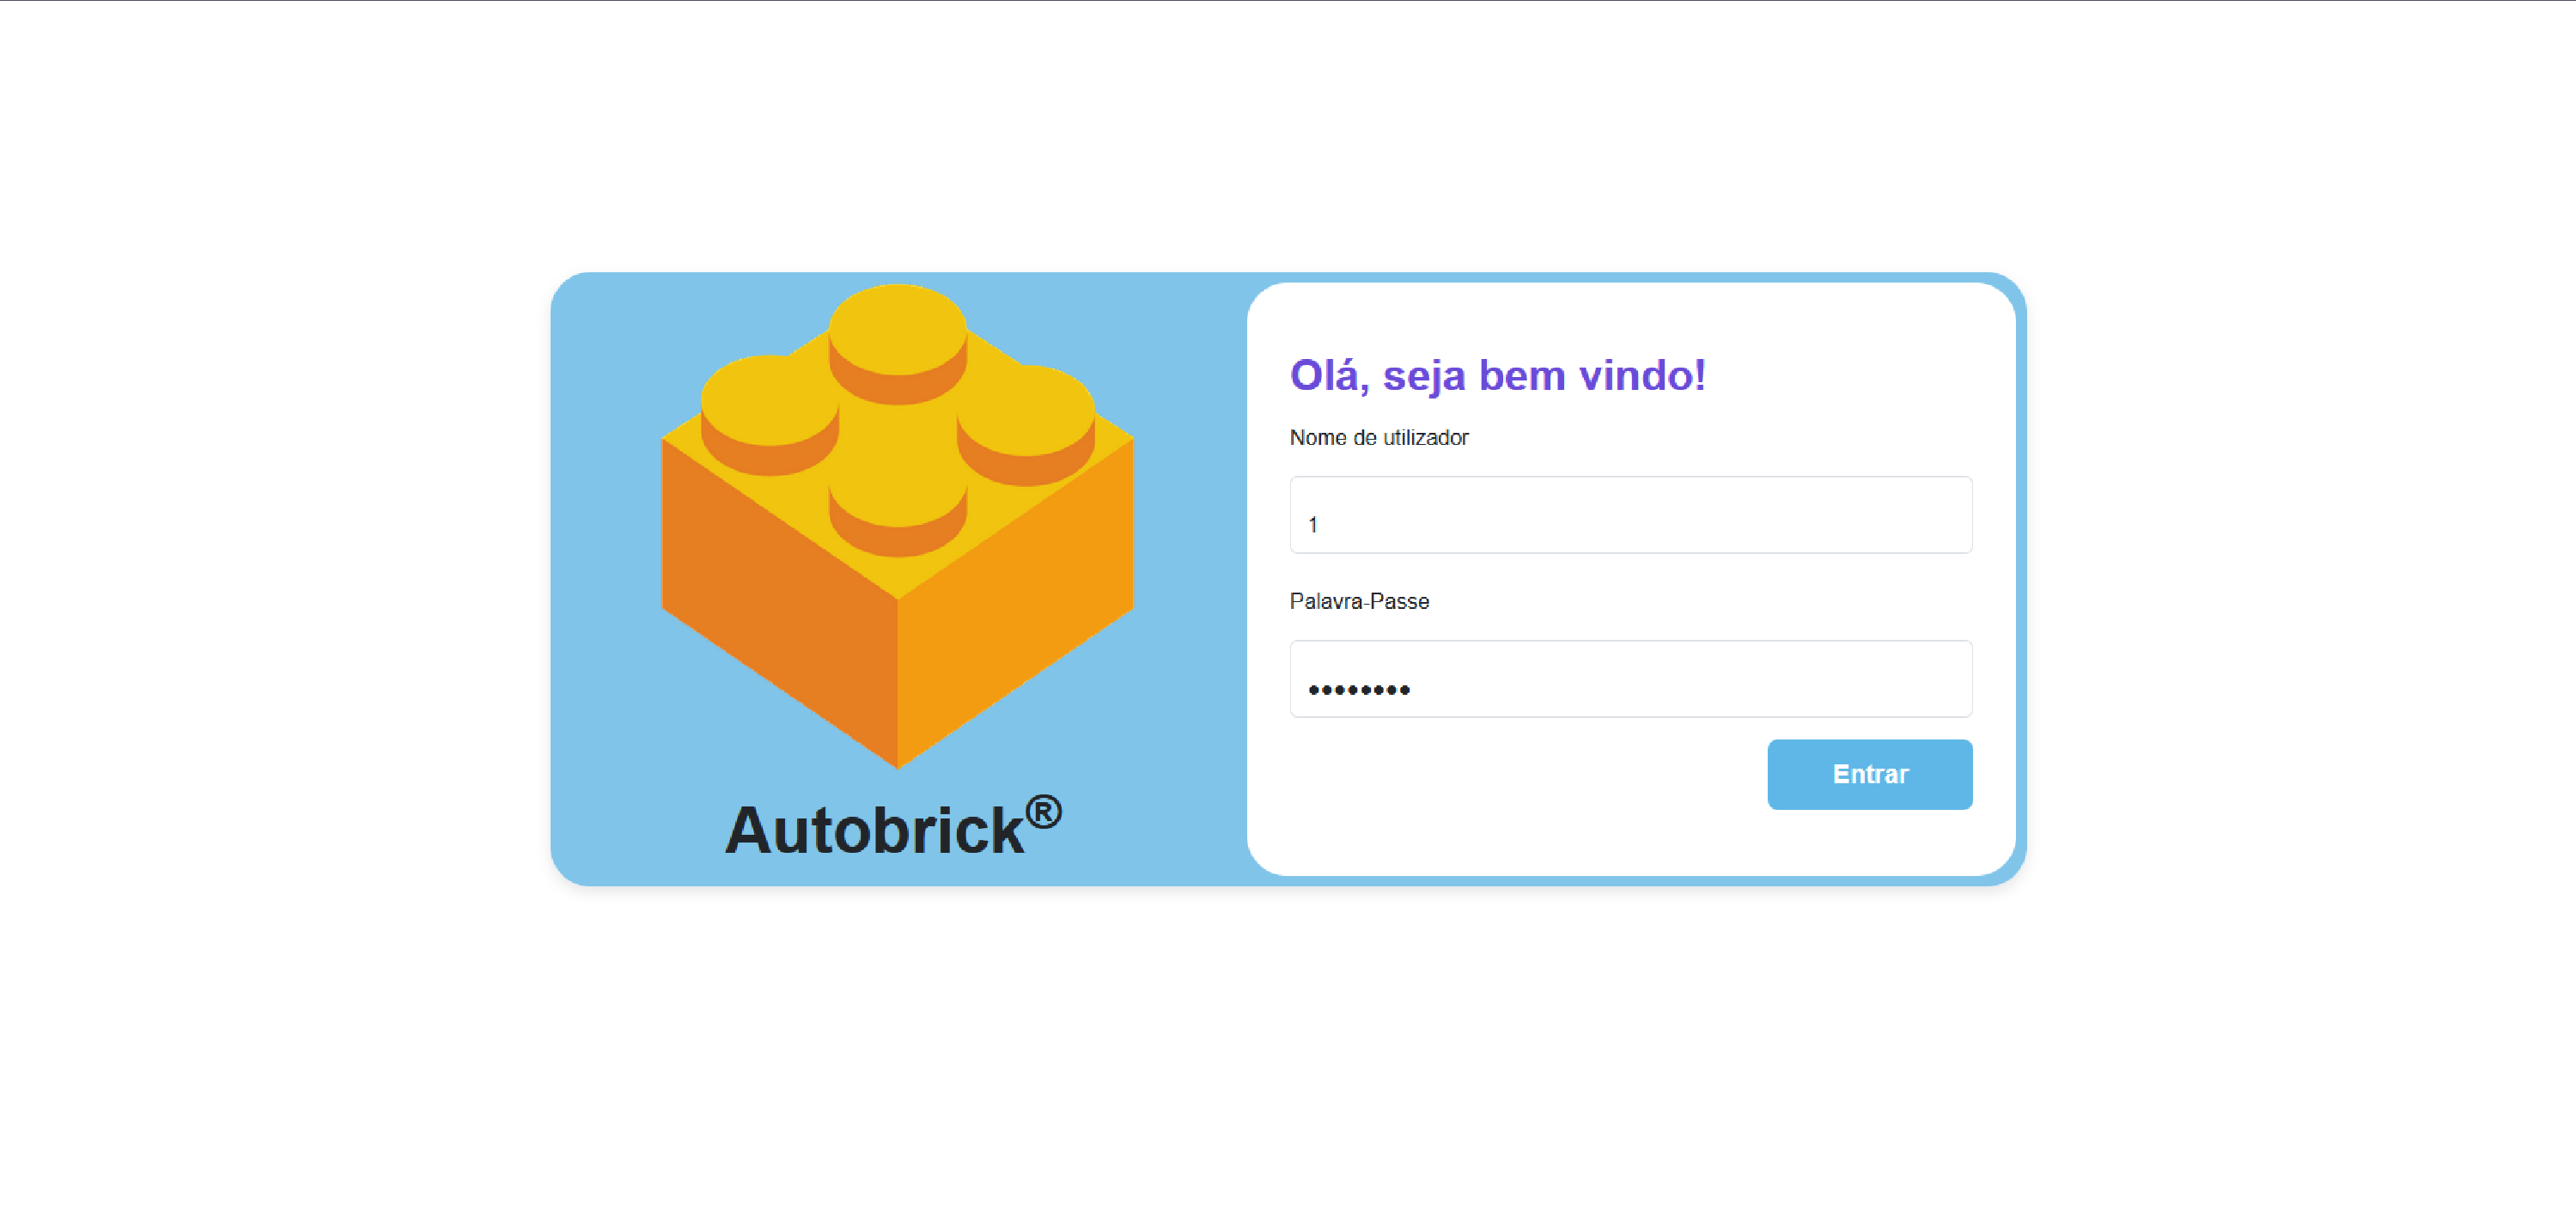
\includegraphics[width=0.8\linewidth, frame]{images/Site/Login.pdf}
                                \caption{Página de início de sessão}
                                \label{fig:Página de login}
                            \end{figure}

                            \begin{figure}[h!]
                                \centering
                                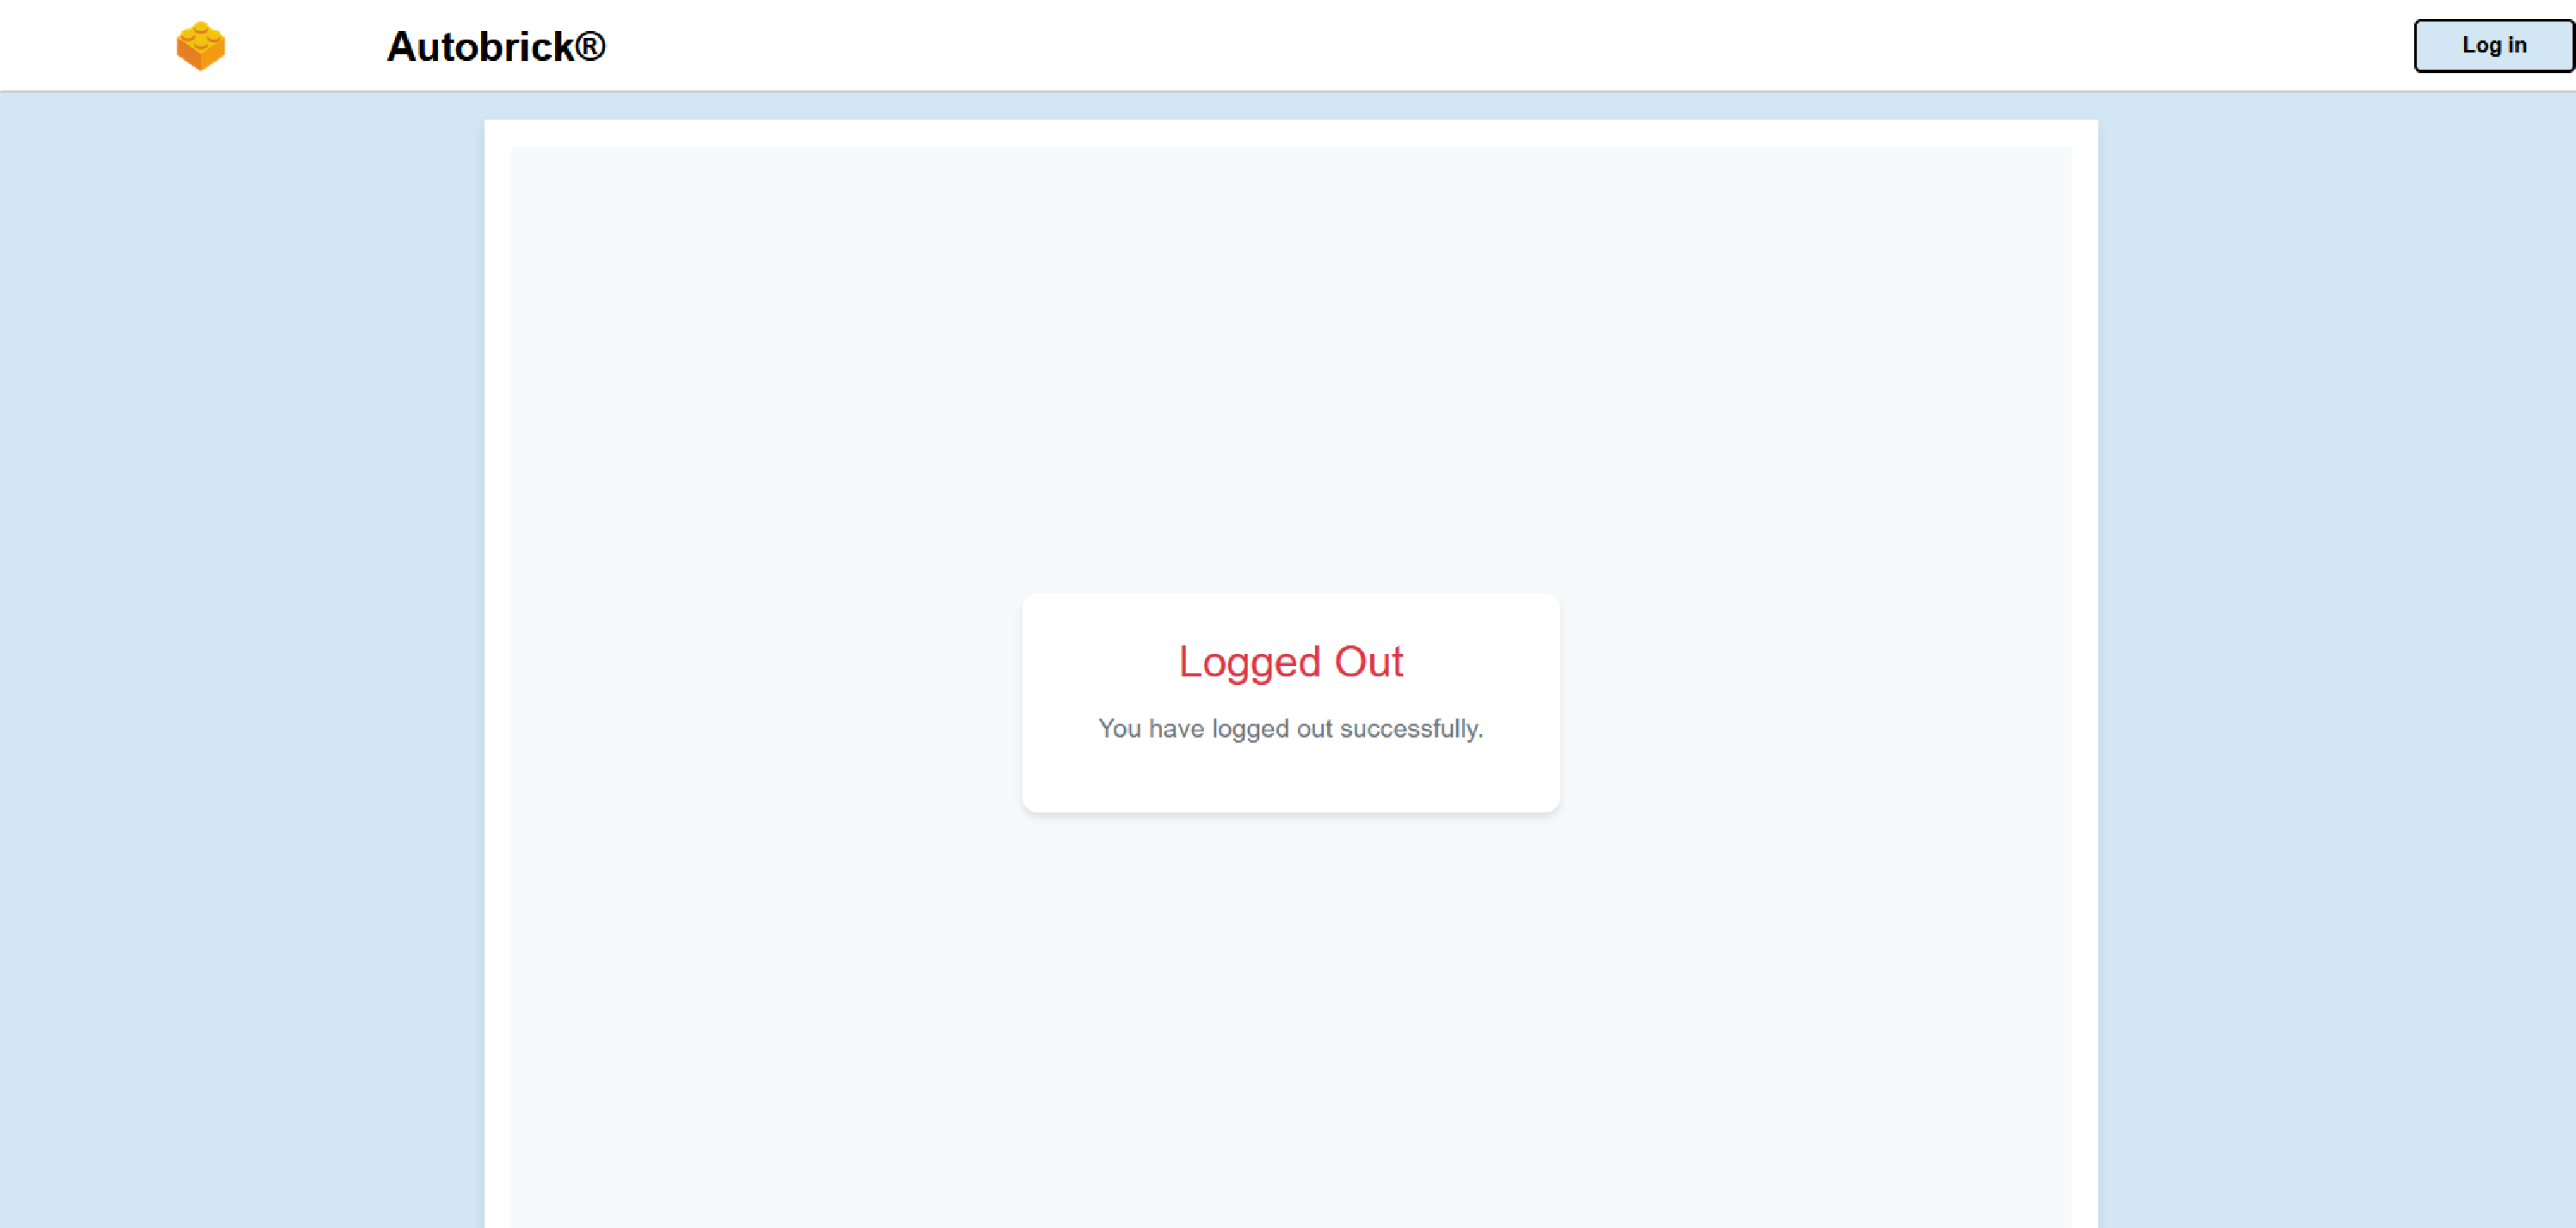
\includegraphics[width=0.8\linewidth, frame]{images/Site/Logout.pdf}
                                \caption{Página de término de sessão}
                                \label{fig:Página de logout}
                            \end{figure}

                    Estsa são as páginas vistas antes do início de sessão no sistema e após o término da mesma (ver requisitos 2.2.2/2.2.3). O que é inserido nos campos é submetido a verificação contra as credenciais armazenadas na base de dados (ver 2.2.1). Não é percetível, mas note-se adicionalmente que a sessão é guardada em cookie de autenticação com 30 minutos de validade. Assim, se não se terminar a sessão, é possível fechar e voltar a abrir o sistema dentro desse espaço de tempo sem precisar de iniciar sessão de novo.

                    % Satisfaz Reqs...
                        % 2.2.1 (teste de validade de senha)
                        % 2.2.2/3 (início/término de sessão)
                        % 2.2.4 (detalhes da conta, ao ver nome na barra superior)
                    % Explicar mantimento de sessão via cookie de autenticação com 30 minutos de vida (ver Program.cs) 

            \clearpage
            \subsection{Serviços Relativos a Encomendas}
                \subsubsection{Consultar Encomendas Pendentes}

                            \begin{figure}[h!]
                                \centering
                                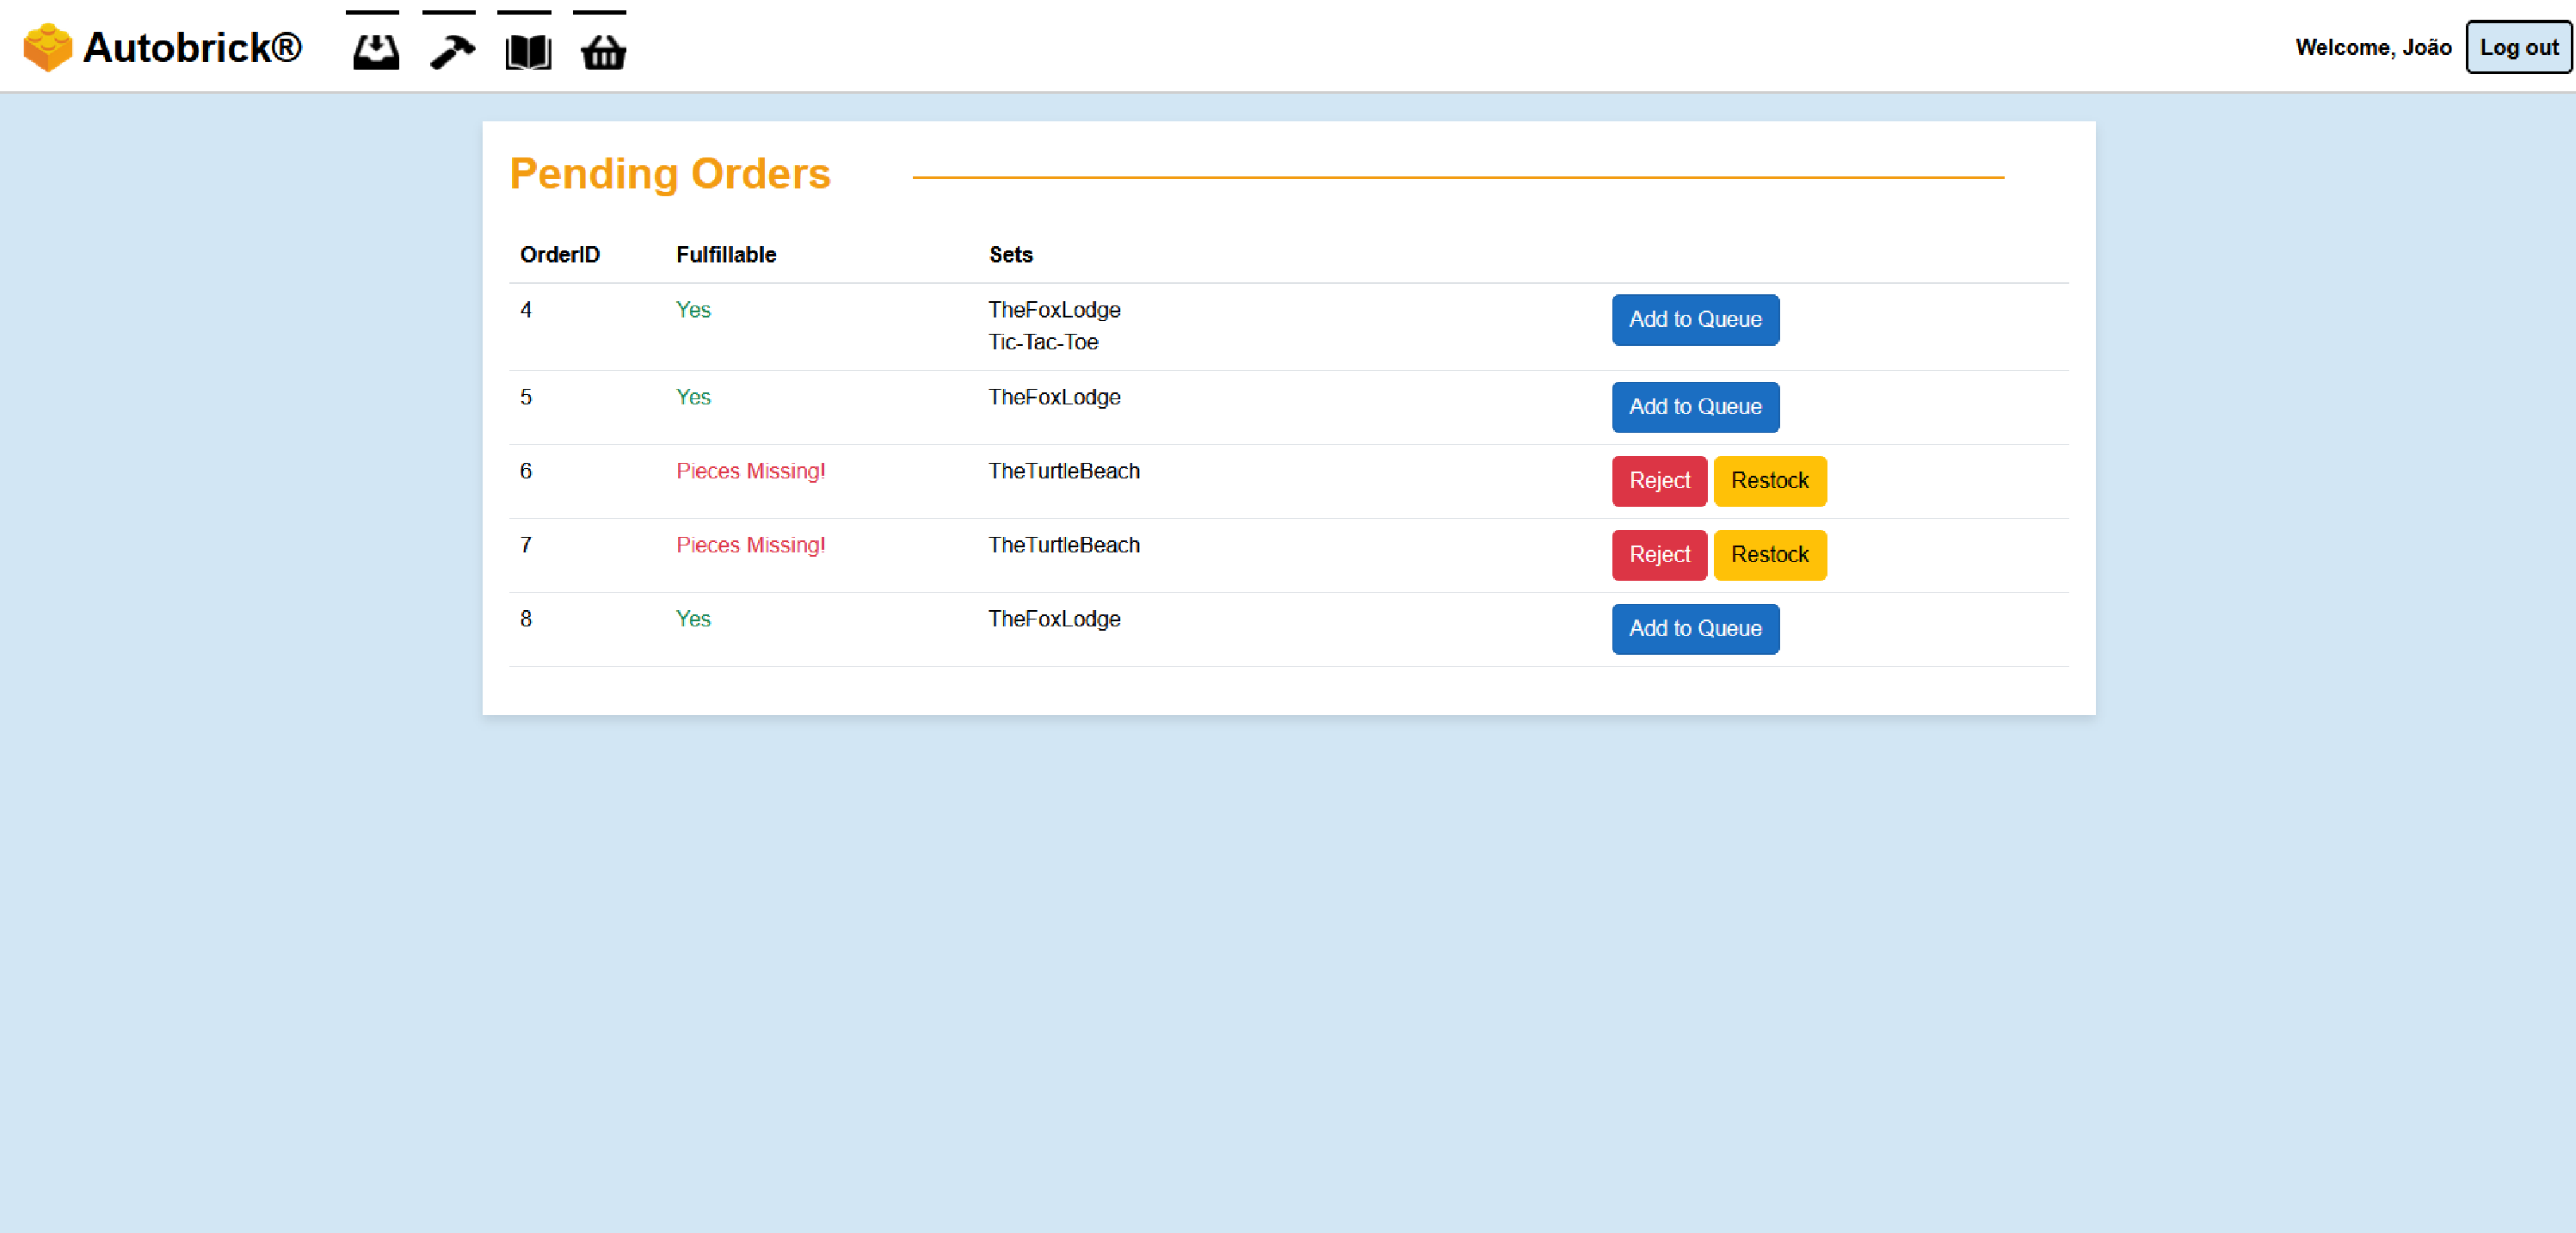
\includegraphics[width=0.8\linewidth, frame]{images/Site/Pending Orders.pdf}
                                \caption{Página de encomendas pendentes}
                                \label{fig:Página de encomendas pendentes}
                            \end{figure}

                    Nesta página o utilizador pode consultar todas as encomendas pendentes (ver 2.3.1) bem como analisar a sua viablidade (ver 2.3.2). Após analisada ele pode adicioná-la à fila de montagem (ver 2.3.4), recusar (ver 2.3.3) ou encomendar as peças que não estão disponíveis tendo em conta todos os modelos que inclua (ver 2.4.3). Pode ainda consultar o seu nome de utilizador através da barra de navegação (ver 2.2.4).

                
                    % Satisfaz Reqs...
                        % 2.3.1 (consultar encomendas pendentes)
                        % 2.3.2 (viabilidade de encomenda pendente)
                        % 2.3.3 (recusar encomenda pendente)
                        % 2.3.4 (colocar encomenda pendente em fila)
                        % 2.4.3 (reposição automática com base em peças que faltem a encomenda)
                \subsubsection{Consultar Fila de Montagem de Encomendas}
                    
                    \begin{figure}[h!]
                        \centering
                        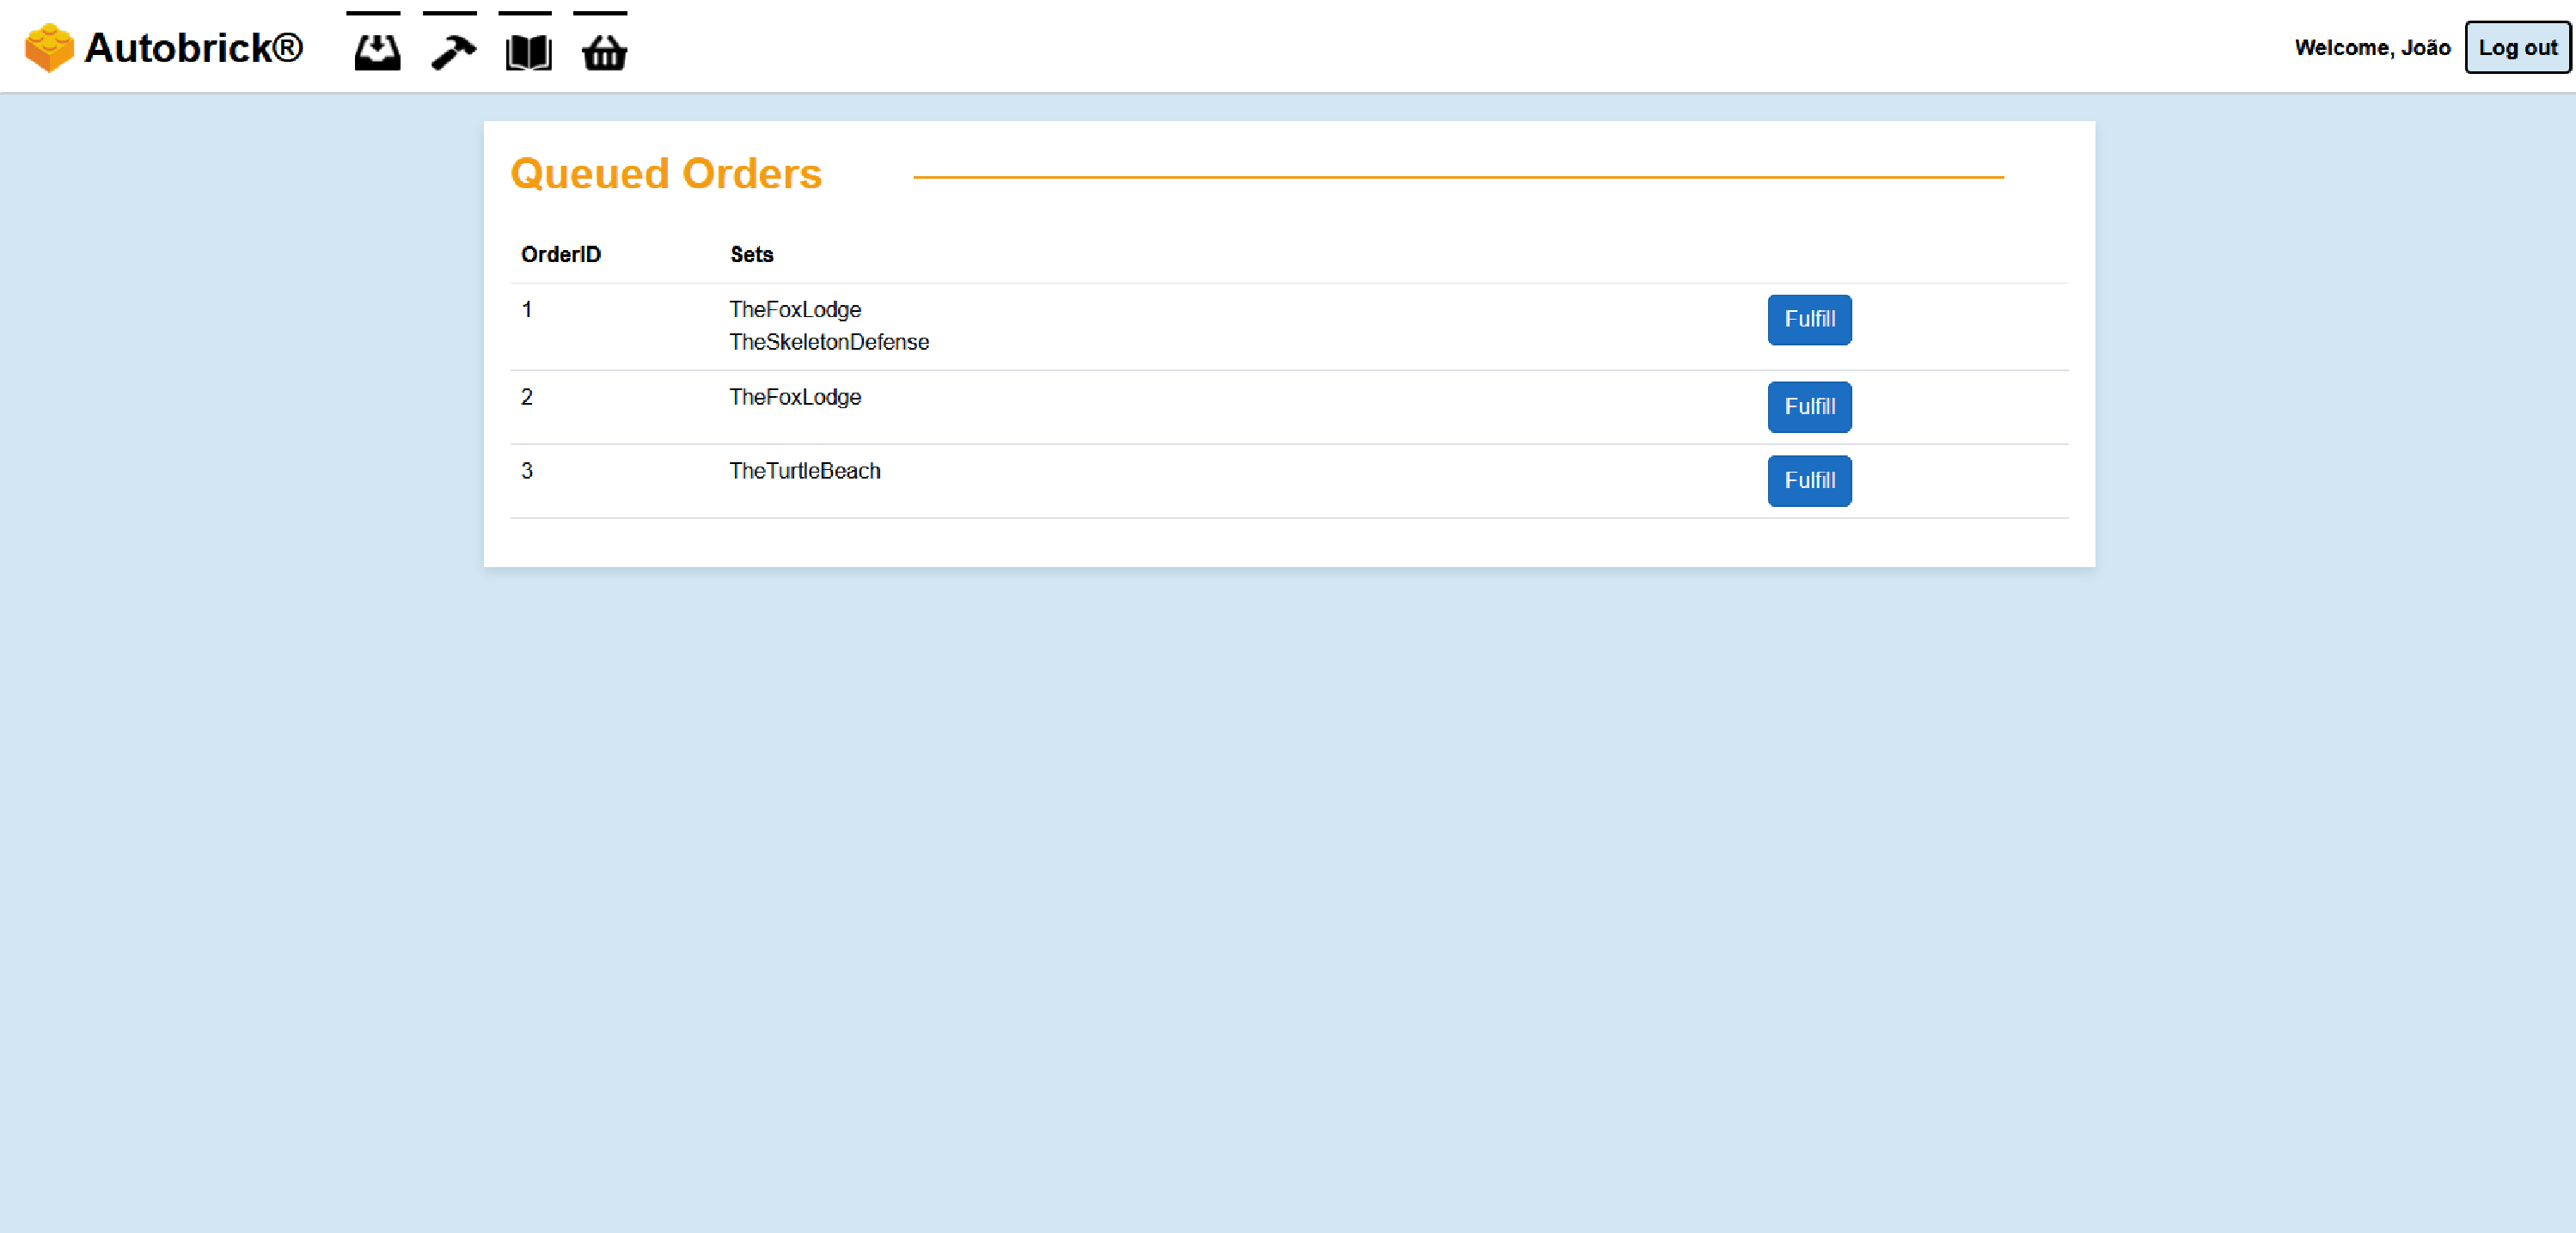
\includegraphics[width=0.8\linewidth, frame]{images/Site/Queued Orders.pdf}
                        \caption{Página de fila de montagem de encomendas}
                        \label{fig:Página de fila de montagem de encomendas}
                    \end{figure}

                    Esta página contem todas as encomendas que foram colocadas em fila de montagem (ver 2.3.5). Aqui o utilizador pode arrancar com a montagem de uma encomenda (ver 2.3.6) e posteriormente marcar essa encomenda como finalizada (ver 2.3.7).

                    % Satisfaz Reqs..
                        % 2.3.5 (consulta da fia de montagem)
                        % 2.3.6 (arrancar fila de montagem - simplificado para consulta de modelos intra-encomenda)
                        % 2.3.7 (confirmar montagem de modelo em encomenda - simplificado para finalização geral da encomenda)

            \subsection{Serviços Relativos a Modelos}
                \subsubsection{Consulta a Catálogo de Modelos} % 2.5.1 (consultar catálogo de modelos)

                    \begin{figure}[h!]
                        \centering
                        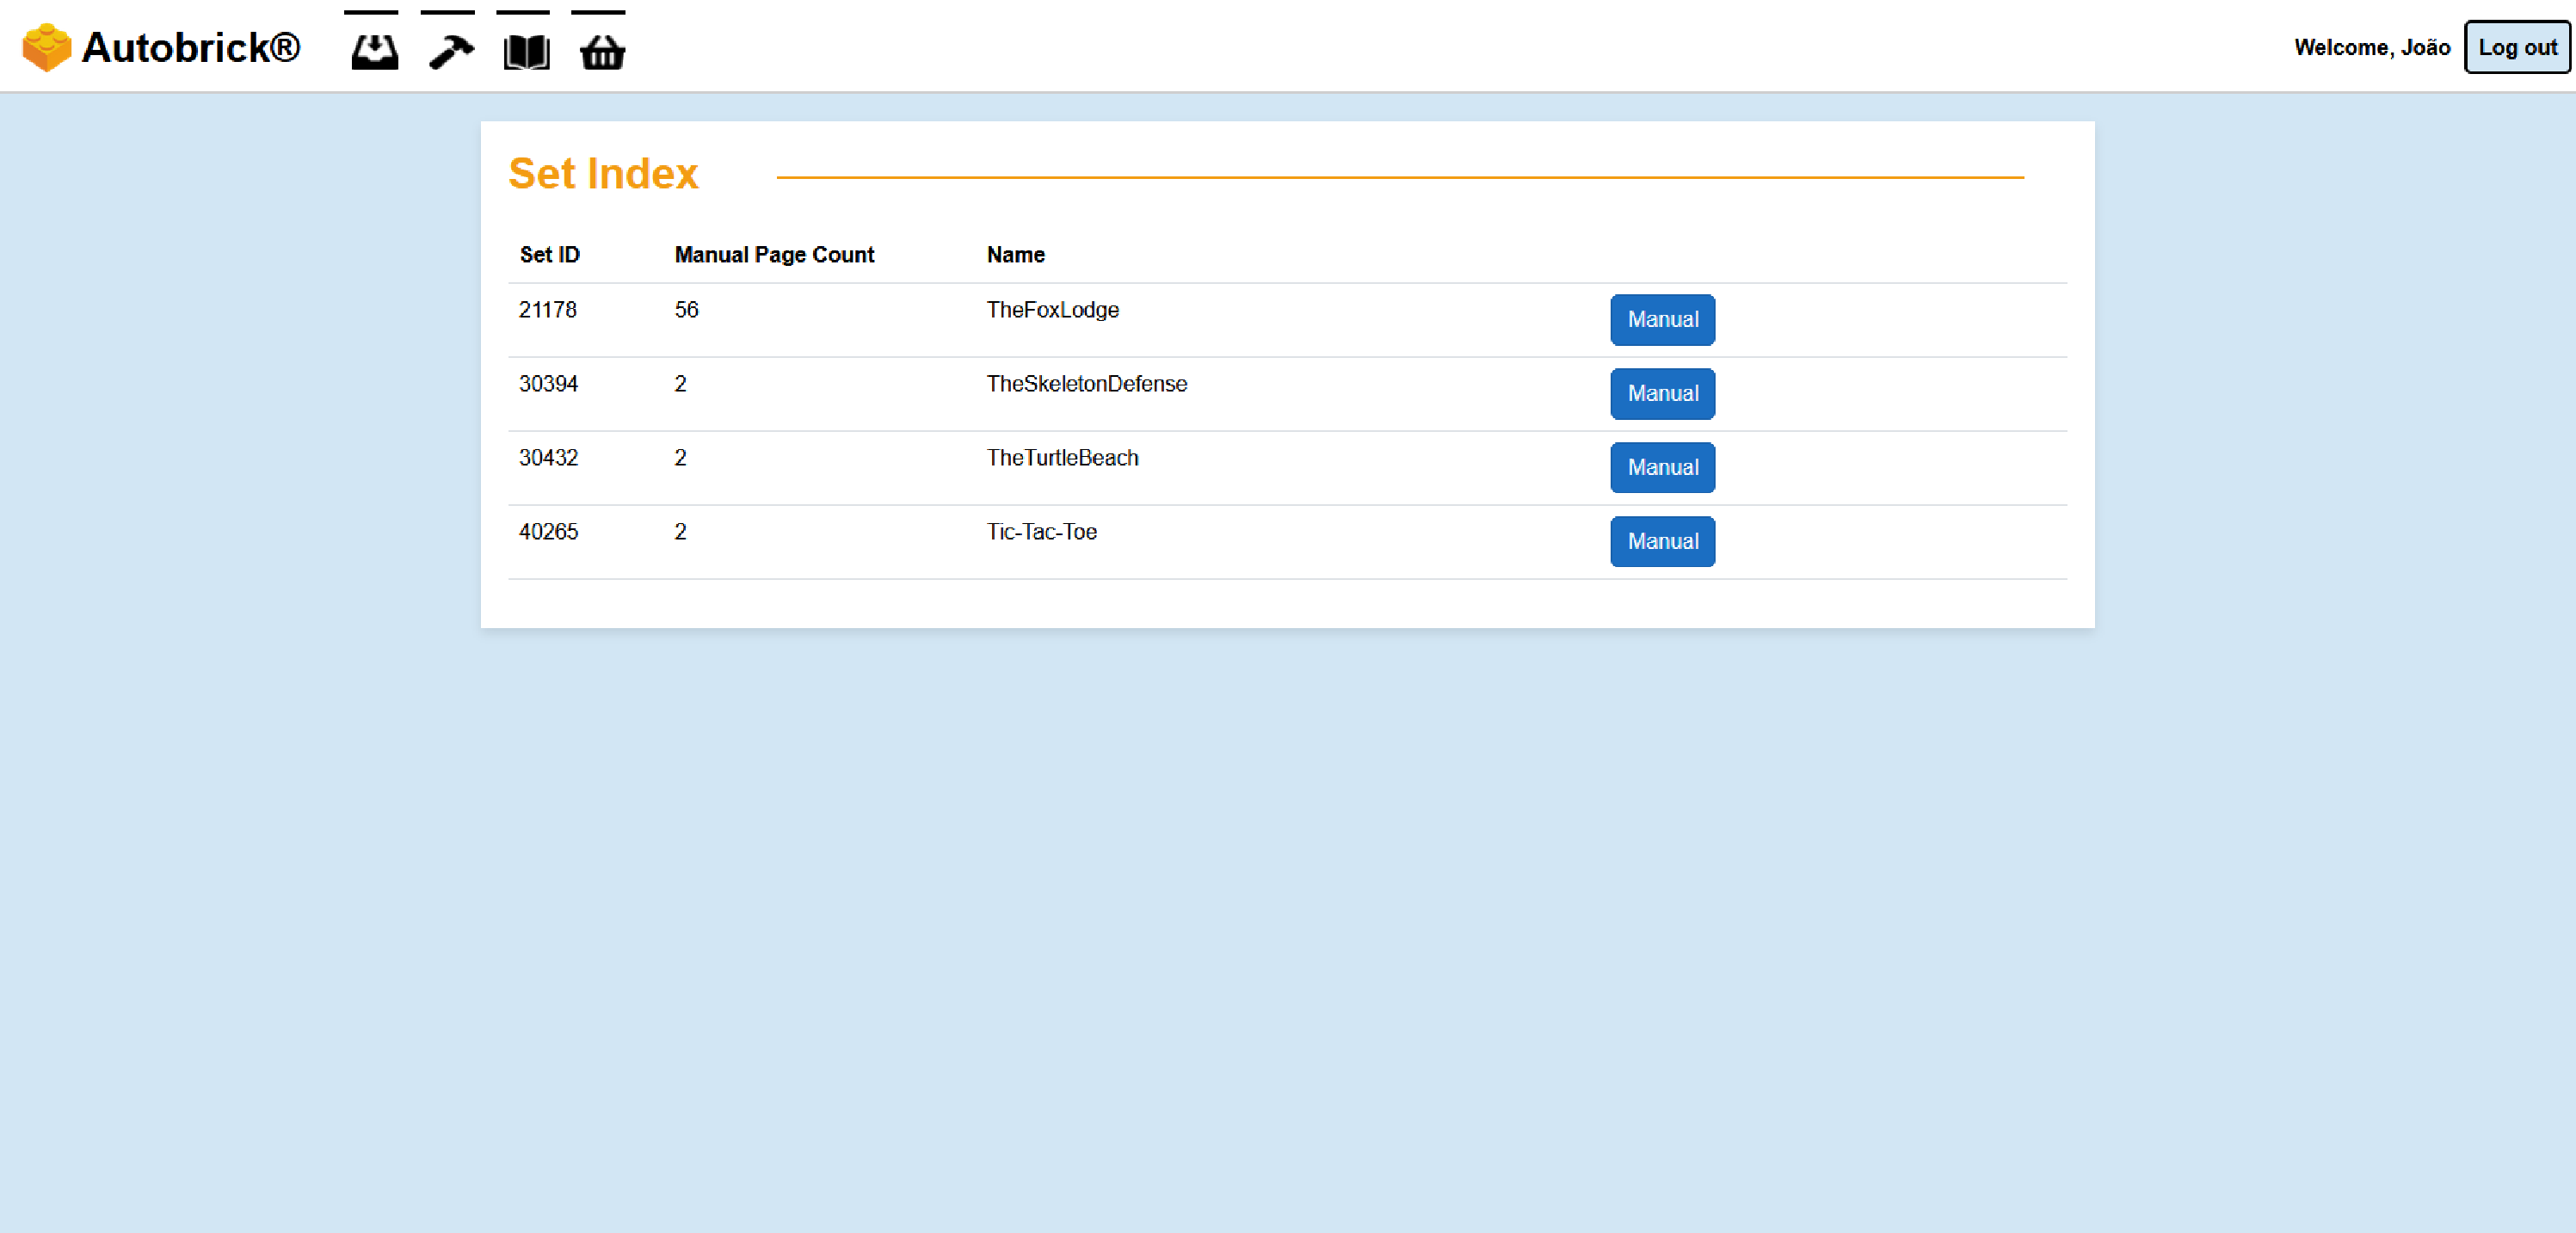
\includegraphics[width=0.8\linewidth, frame]{images/Site/Set Index.pdf}
                        \caption{Página de catálogo de modelos}
                        \label{fig:Página de catálogo de modelos}
                    \end{figure}

                    Nesta página está disponível uma lista com todos os modelos registados no sistema bem como a possibilidade de ver o manual de um modelo que pretender (ver 2.5.2 e 2.5.3)

                    
                \subsubsection{Visualizar Sequência de Montagem de Modelo}
                    
                    \begin{figure}[h!]
                        \centering
                        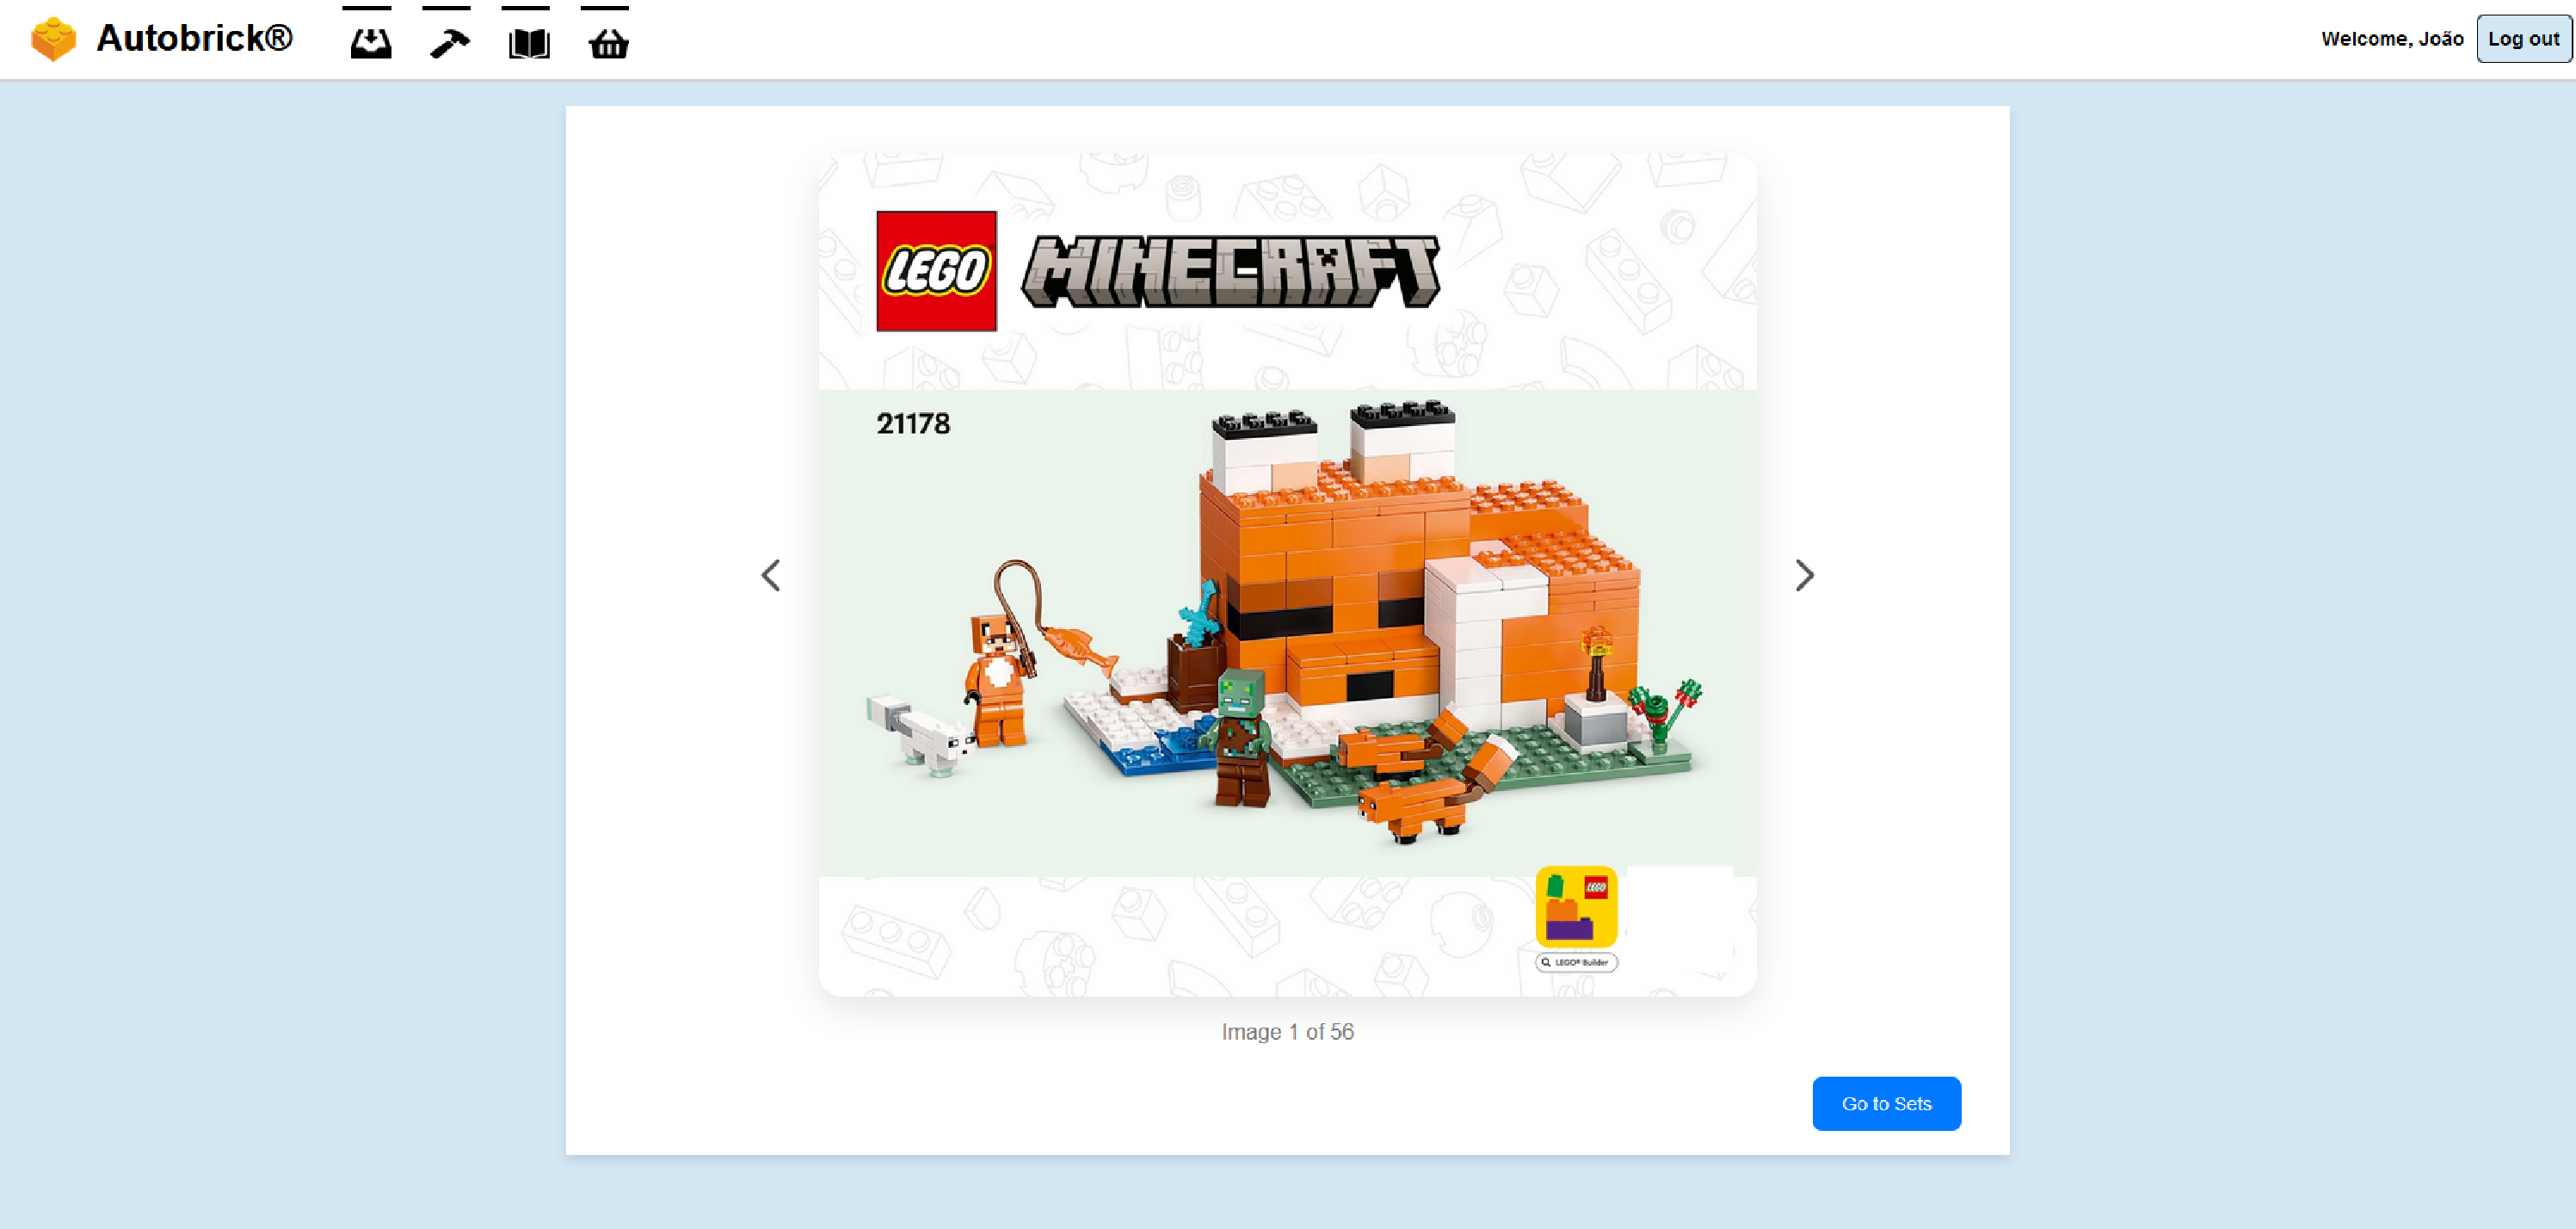
\includegraphics[width=0.8\linewidth, frame]{images/Site/Manual.pdf}
                        \caption{Página com sequência de montagem de modelo}
                        \label{fig:Página de fila de montagem de encomendas}
                    \end{figure}

                    Aqui temos a página do manual do respetivo modelo onde o utilizador pode andar para a frente e para trás no manual ou voltar à lista de modelos.
                    
                    % Satisfaz Reqs...
                        % 2.5.2 (visualizar montagem de modelo)
                        % 2.5.3 (existência de manual para modelo // nao-funcional)

            \subsection{Serviços Relativos ao Inventário}
                
                \subsubsection{Consulta a Inventário de Peças} % Req. 2.4.1
                    
                    \begin{figure}[h!]
                        \centering
                        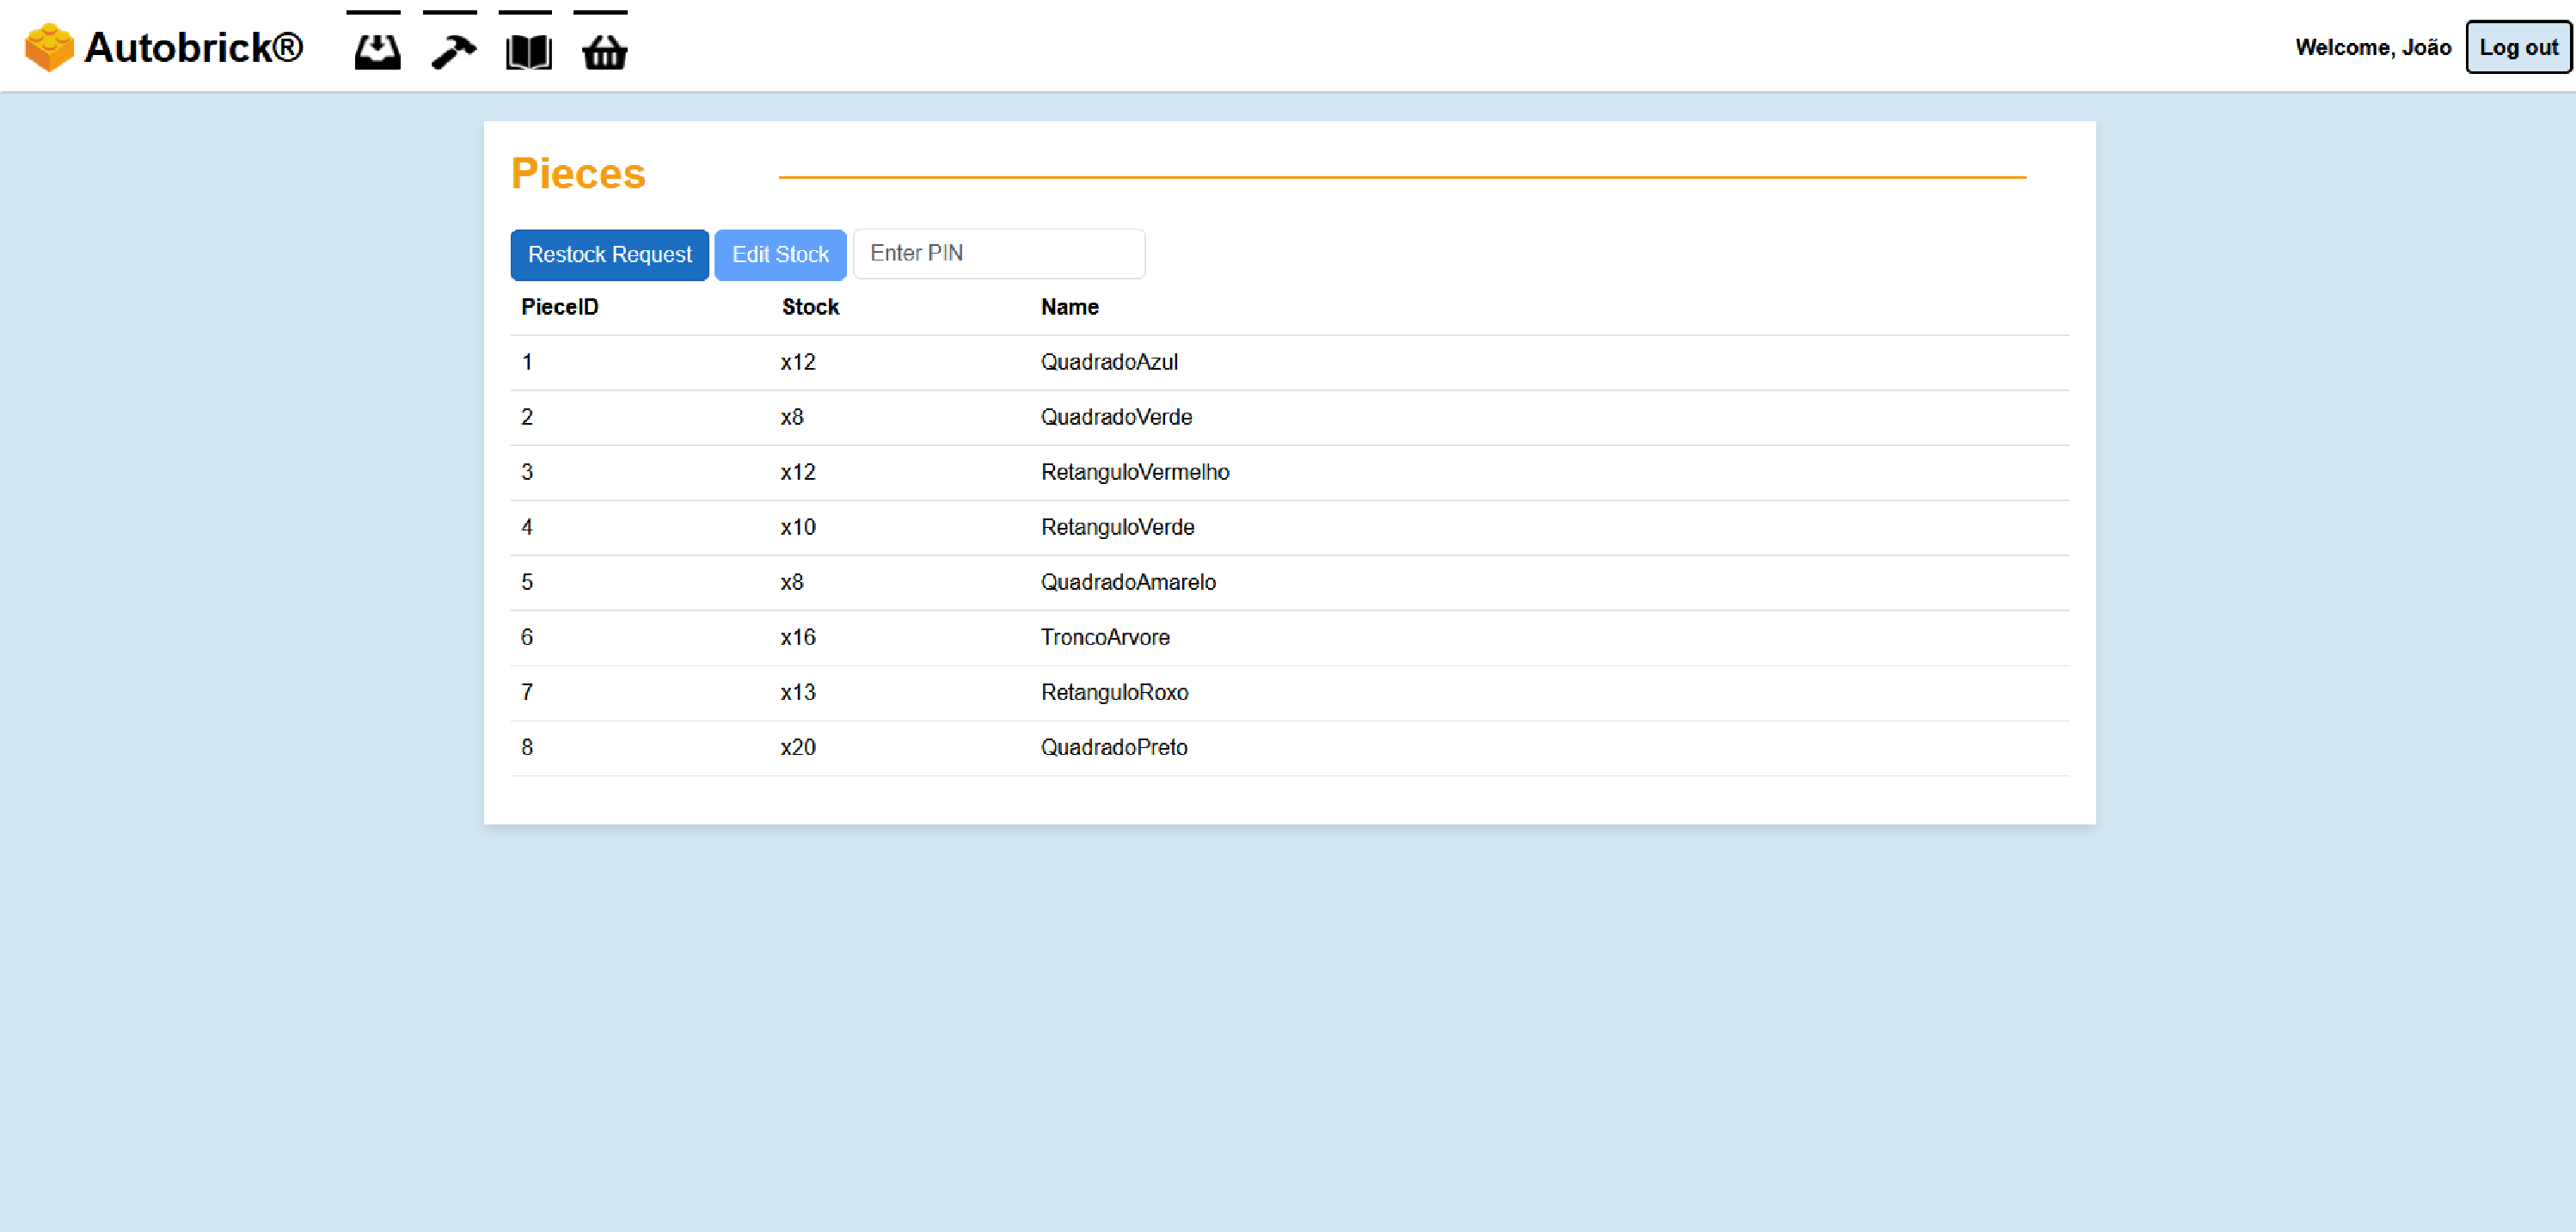
\includegraphics[width=0.8\linewidth, frame]{images/Site/Inventory.pdf}
                        \caption{Página de inventário de peças}
                        \label{fig:Página de inventário}
                    \end{figure}

                    A página para consulta do inventário (ver requisito 2.4.1) apresenta todas as peças cujas quantidades disponíveis sejam não-nulas. É a partir daqui que se tem acesso à página para pedido de reposição e, após inserção dum código administrativo válido, à página de edição do inventário atual.
                
                \subsubsection{Pedido de Reposição Manual de Inventário} % Req 2.4.2 

                    \begin{figure}[h!]
                        \centering
                        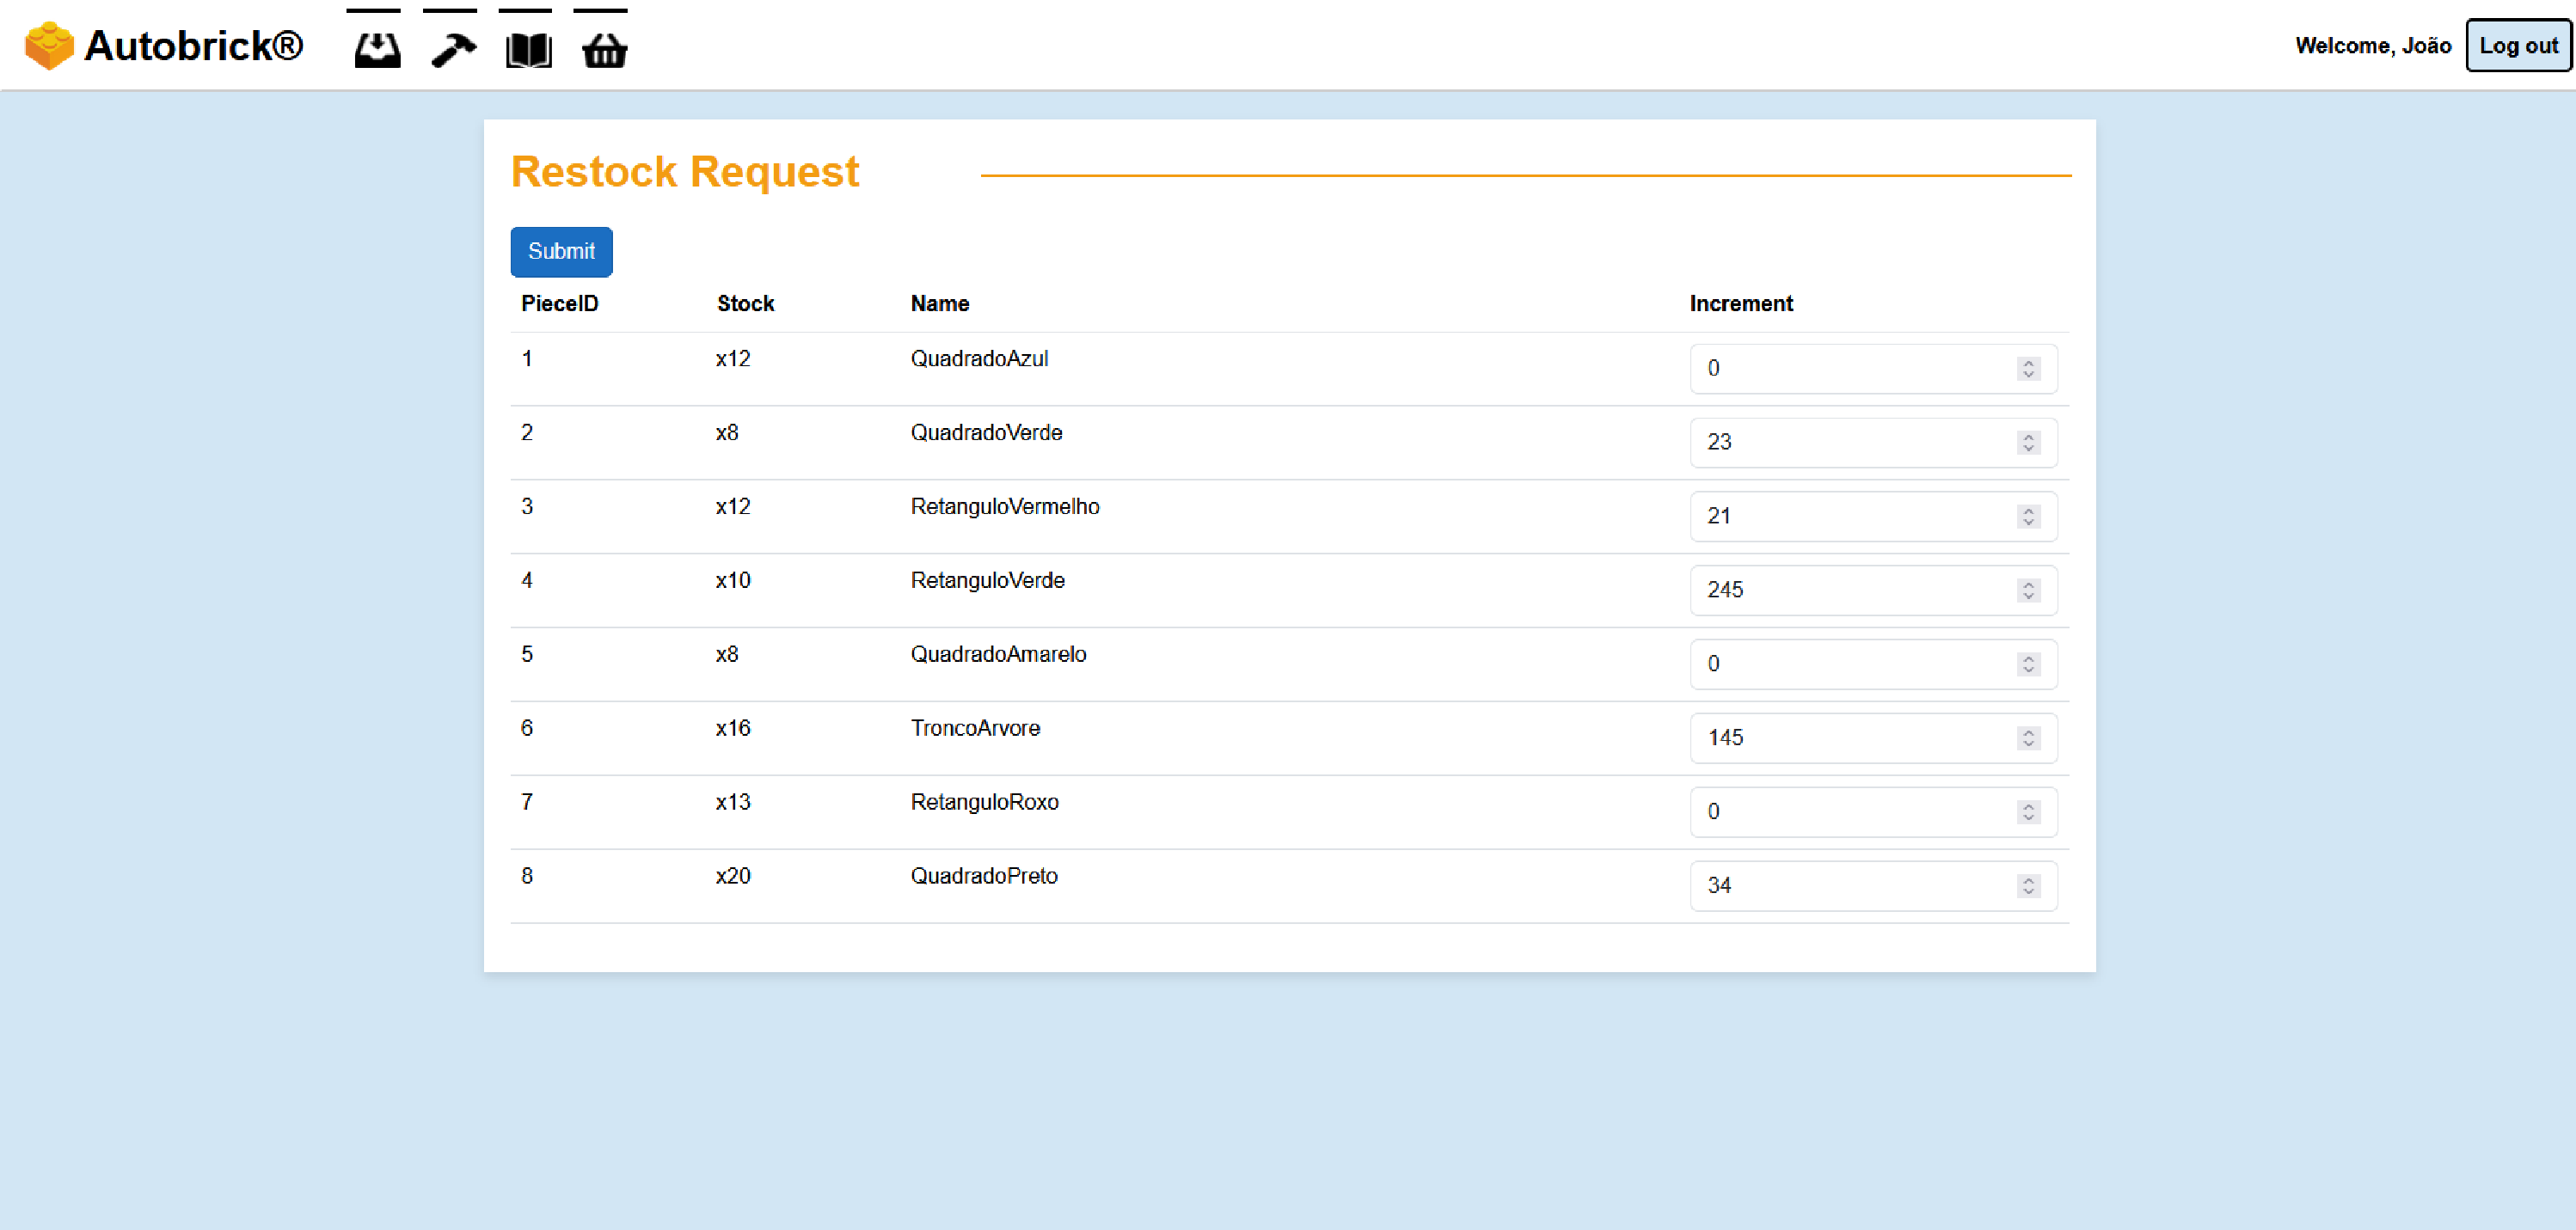
\includegraphics[width=0.8\linewidth, frame]{images/Site/Restock.pdf}
                        \caption{Página de pedido de reposição de inventário}
                        \label{fig:Página de pedido de reposição de inventário}
                    \end{figure}

                    A página de pedido de reposição manual está disposta de modo a que todos os valores inseridos nos campos causem incrementação aos atuais valores de quantidade unitária nas correspondentes peças ao pressionar o botão \textit{Submit}.
                
                \subsubsection{(Administrativo) Editar Quantidades em Inventário} % Req 2.4.4

                    \begin{figure}[h!]
                        \centering
                        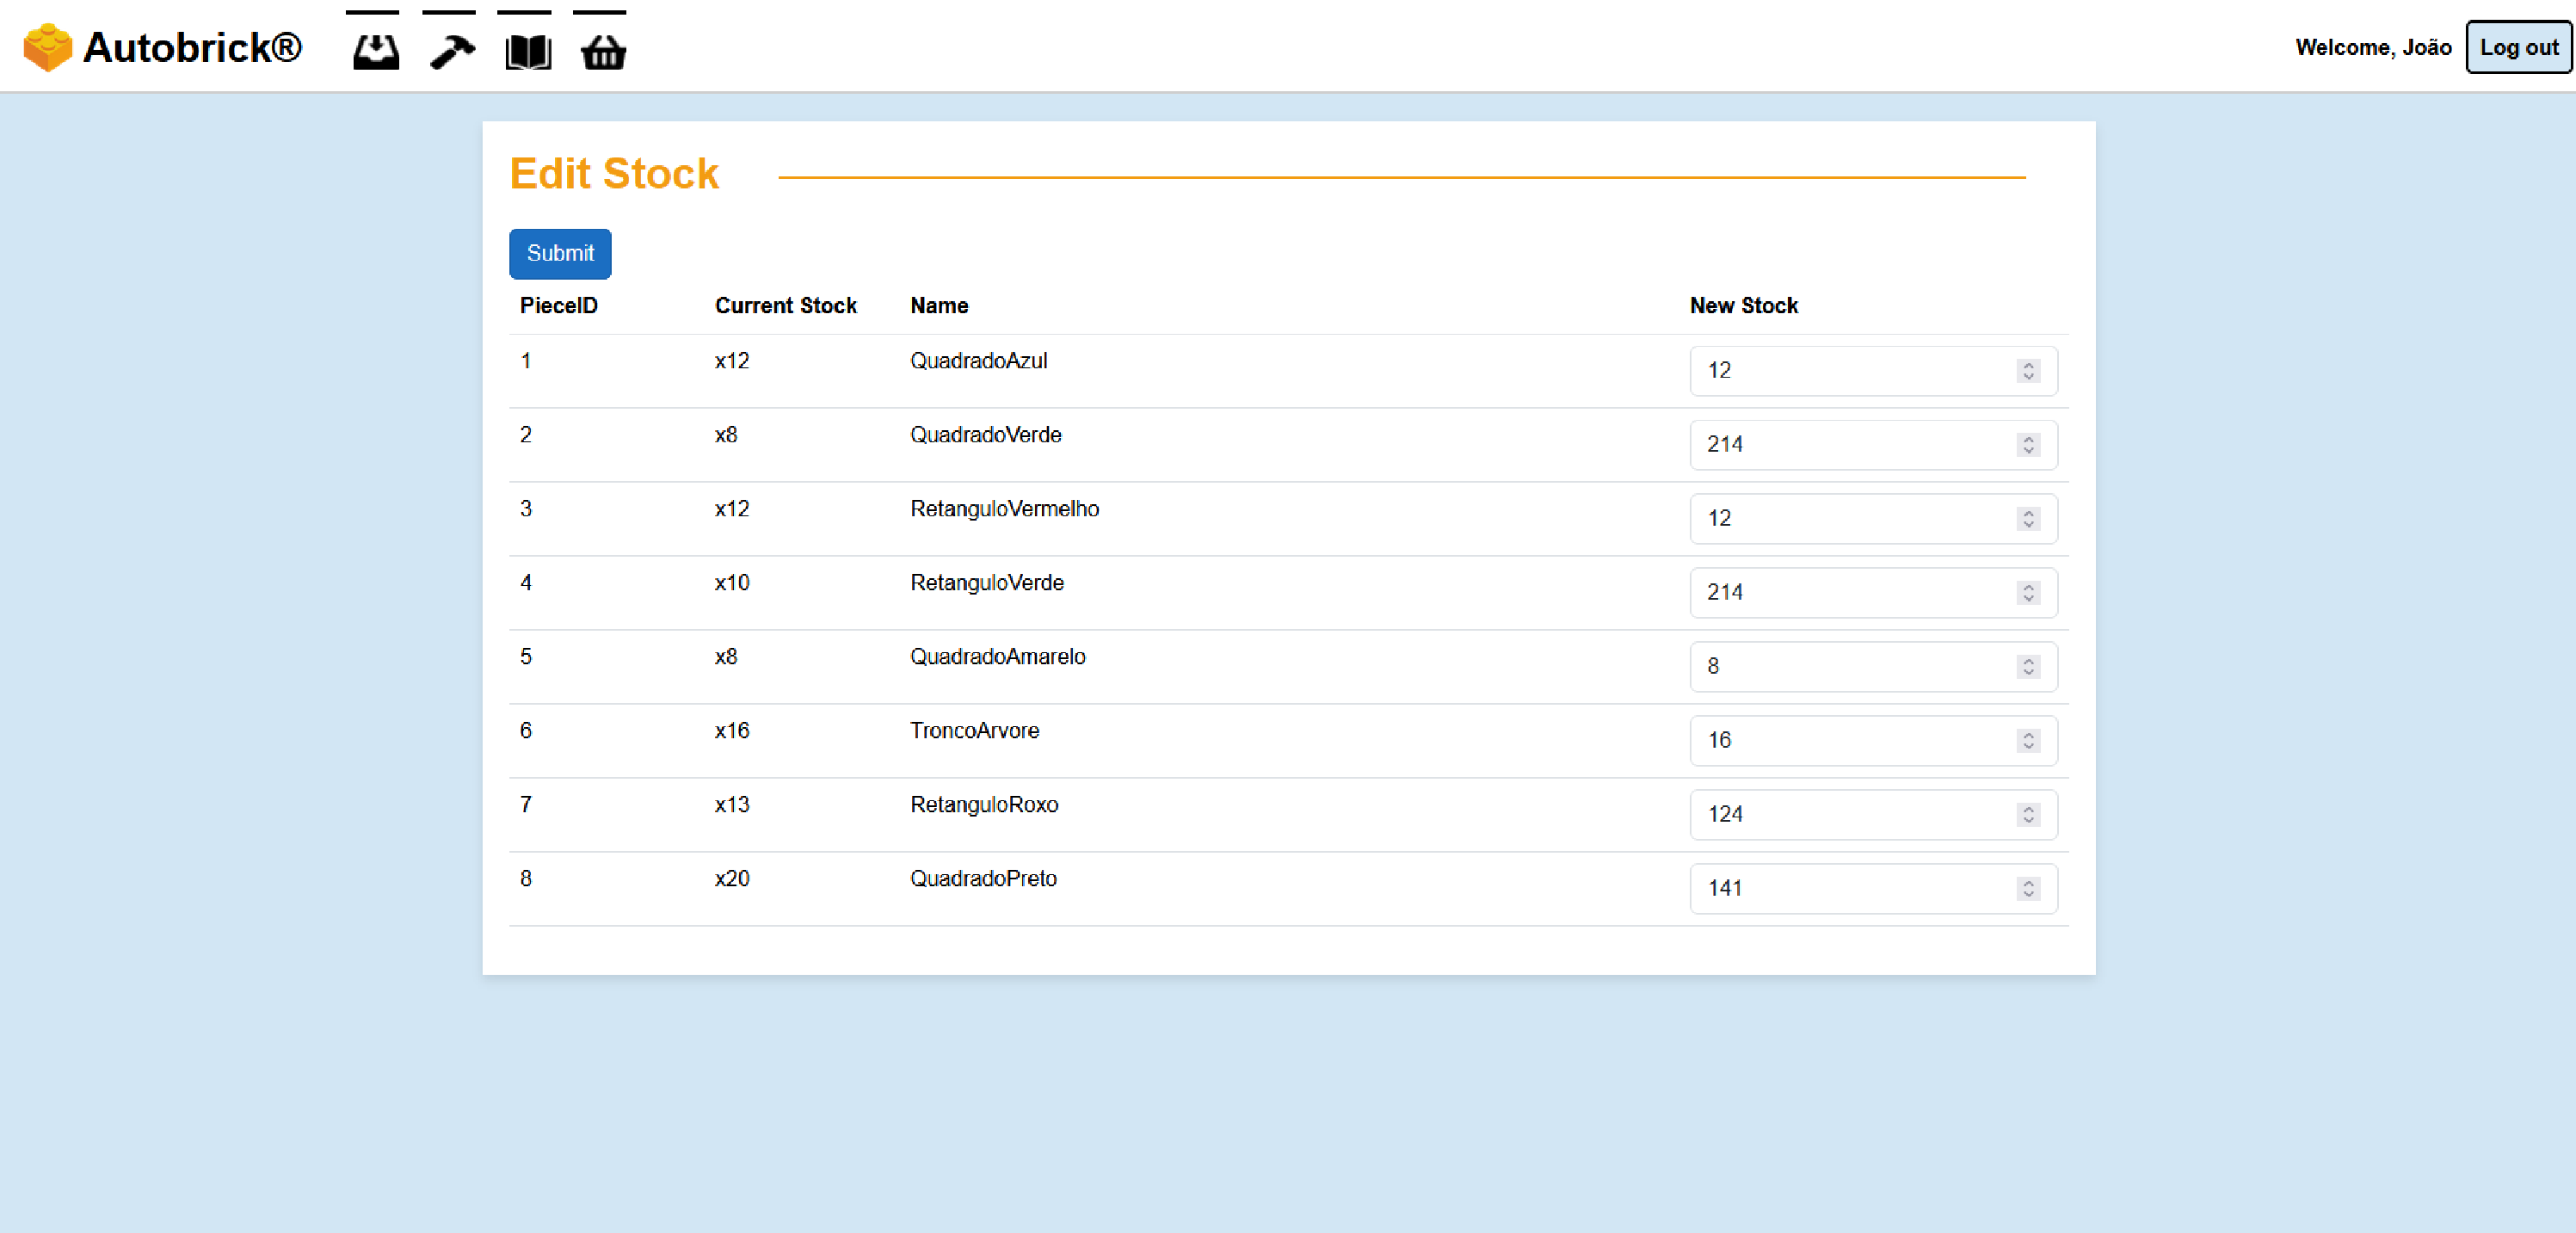
\includegraphics[width=0.8\linewidth, frame]{images/Site/EditStock.pdf}
                        \caption{Página de edição das quantidades em inventário}
                        \label{fig:Página de edição das quantidades em inventário}
                    \end{figure}    

                    Esta página apenas é acessível com uma chave de administrador e dá acesso à manipulação manual do inventário (ver 2.4.4). Após a confirmação, todos os valores inseridos irão sustituir aqueles que estavam previamente registados na página de stock.
        
    \newpage
    \section{Análise e Avaliação de Desempenho}

        \subsection{No Acesso a Dados}
        
        Confronto da implementação com os princípios ACID:
        \begin{itemize}
            \item Atomicidade: os métodods dos DAOs estão escritos de forma a haver rollback se qualquer exceção ocorrer.
            \item Consistência: qualquer das alterações à base de dados está estabelecida de modo a preservar integridade referencial. isto é especialmente crítico na rejeição de encomendas, dada a existência da tabela de junção entre uma encomenda e um modelo.
            \item Isolamento: não aplicável, pois a aplicação não recorre a programação concorrente.
            \item Durabilidade - não se fazem \textit{logs} ou registos de histórico de transações, algo que lhes acrescentaria resistência perante falhas de \textit{hardware}. No entanto, não há um mantimento prolongado de dados em memória volátil.
        \end{itemize}
        
        \subsection{Na Execução dos Serviços}
            
            O objetivo principal ao executar um serviço é que este seja o mais rápido e simples possível para o utilizador devido ao seu público-alvo e local de aplicação. A aplicação apresenta ao uma página de log in que permite ao mesmo autenticar-se para iniciar o trabalho. Ao utilizar a aplicação no contexto de aquisição de encomendas, a mesma garante que em tempo real o utilizador escolha que encomendas pretende efetuar, e em caso de ser necessário efetuar um pedido de restock para conseguir realizar a mesma. Permite controlar o inventário em tempo real, tendo atualização constante das peças que estão disponíveis para montagem e em caso de ser necessário o utilizador consegue efetuar um pedido de restock. No contexto de linha de montagem em si, o utilizador consegue ler o manual de instruções enquanto monta a peça, o mesmo permite passar a página e voltar para a anterior em tempo real. 
    
%==========================================================================
% END #6 - IMPLEMENTAÇÃO
%==========================================================================
%==========================================================================
% BEGIN #7 - CONCLUSOES E TRABALHO FUTURO
% Breve abordagem crítica ao trabalho realizado nesta primeira etapa, referindo aspetos positivos e negativos que acharem dignos de realce, acompanhada, quando necessário, com a exposição de algumas linhas de orientação para trabalho futuro com vista à correção ou melhoramento de tudo aquilo que foi realizado nesta primeira parte do trabalho.
%==========================================================================

\chapter{Conclusões e Trabalho Futuro}

    \section{Conclusão}

        Ao longo das diferentes fases concretizadas, desde a contextualização inicial até à implementação, identificámos um conjunto de detalhes dignos duma análise \textit{a posteriori}.
         
        Entre os aspetos mais positivos, há particular orgulho no levantamento e análise de requisitos, que possibilitou um estabelecimento e discernimento afinado e rigoroso das funcionalidades pretendidas.
        
        Foram feitas várias reformulações e correções ao longo do projeto. A de maior magnitude deu-se na inicial existência duma conta de administrador que, para além de herdar os casos de uso dirigidos ao utilizador normal, seria capaz do caso de uso de edição de quantidades disiponíveis das peças no inventário. Dado que o sistema é orientado a um único cargo de trabalho e só haveria esta operação como diferença, usou-se antes a estratégia mais "ligeira" de deixá-la acessível a todos os utilizadores, porém atrás duma senha administrativa.
        
        Uma outra, relacionada com o relatório, foi a primeira interpretação como objetivos do sistema (ver subcapítulo 1.3) os pontos enumerados atualmente na justificação do sistema (ver subcapítulo 1.5), e a maquete inicial foi substituída por uma que melhor representa o funcionamento pretendido, dando pistas sobre tanto as camadas de dados como as de lógica e apresentação.

        Com o decorrer da implementação foi necessária a revisão e atualização da base de dados.

        Foi decidido ainda com concordância dos clientes, mudar um pouco a interface e apresentação do programa para eliminar burocracias, tornar o design mais compacto, e garantir uma maior produtividade e simplificação da utilização da aplicação para oferecer um maior workflow.
        
        Olhando para trás, reconheceu-se que a funcionalidade de pedidos de inventário acrescentou complexidade não insignificante ao sistema. Poderia ter sido descartada sem pôr em causa o proposto no enunciado do projeto - no entanto, materializar essa alteração implicaria demasiado alagamento de trabalho anterior, especialmente na contextualização. 
        
        Houve uma certa omissão no diagrama de Gantt relativa a uma vistoria e emenda periódicas de tarefas previamente concluídas em prol da coerência de contexto. Foram efetuadas no âmbito das reuniões semanais. Não considerámos que tais atualizações fossem de significância cronológica suficiente para as mencionar na secção do planeamento.

        Considerou-se que poderiam ter sido usados mais diagramas na fase de modelação, especialmente um de atividade, de modo a complementar os casos de uso elaborados. Foi algo que ficou por realizar por motivos logísticos.
    
    \section{Trabalho Futuro}

        % cenas de possível acréscimo:
        %% - segurança no armazenamento de senhas
        %% - serviço de criação de encomendas, visto que a implementação atual só permite processamento das mesmas
        %% - arquitetura mais modular:
                %%% pondo a lógica de negócio em controladores de modo a fazer do back end uma API. isto permite mudanças radicais ao front end sem qualquer impacto em camadas abaixo
                %%% estabelecendo subsistemas para melhor divisão de responsabilidades segundo o domínio e os requisitos estabelecidos
        %% - documentação extensa de todas as classes e métodos 
        
        A título de acréscimo futuro à atual implementação, são pertinentes os seguintes serviços e melhorias:
        \begin{itemize}
            \item Segurança no armazenamento de contas. O sistema atual é meramente prova de conceito, visto que as senhas são guardadas em pleno texto ao invés de ser usada encriptação.
            \item Serviço de receção de encomendas. No seu estado atual o sistema apenas serve para processamento de encomendas colocadas pela gestão na base de dados. Seria pertinente a implementação dum mecanismo que conseguisse gerar encomendas a partir dum formato padrão.
            \item Arquitetura mais modular. A lógica de negócio poderia ser completamente transferida para controladores dedicados, separados pelos subsistemas indiciados na especificação da aplicação e enviando objetos de transferência de dados (DTOs) ao \textit{front end}. Isto permitiria ao \textit{back end} ser completamente independente da camada de apresentação, possibilitando até reformulações fundamentais dela sem grande impacto abaixo na cadeia.
            \item Documentação extensa de todas as classes e métodos desenvolvidos.
        \end{itemize}
        
%==========================================================================
% END #7 - CONCLUSOES E TRABALHO FUTURO
%==========================================================================



%==========================================================================
% BEGIN REFERÊNCIAS
%==========================================================================


%% Changes biblibography name
%% Portuguese babel default : "Bibliografia"
%% Personally I prefer "Referências"
\renewcommand\bibname{Referências}

%% https://www.overleaf.com/learn/latex/bibliography_management_with_bibtex
\begin{thebibliography}{9}
    
    \bibitem{Chui2012}
        Chui, M., Manyika, J., Bughin, J., Dobbs, R., Roxburgh, C., Sarrazin, H., Sands, G. e Westergren, M., 2012. «The social economy: Unlocking value and productivity through social technologies» McKinsey Global Institute. Disponível em: \url{https://www.mckinsey.com/industries/technology-media-and-telecommunications/our-insights/the-social-economy} [Acedido em 26 de Novembro de 2024].
        
\end{thebibliography}



%==========================================================================
% END REFERÊNCIAS
%==========================================================================



\end{document}